
%% $Id$

\documentclass[12pt,a4paper,fleqn]{report}
\usepackage{latexsym,graphicx,../iman,../extra,../ttbox,../proof,../rail,../railsetup,../isar,../pdfsetup}

\title{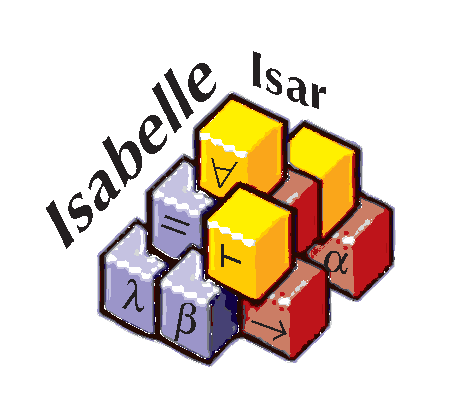
\includegraphics[scale=0.5]{isabelle_isar} \\[4ex] The Isabelle/Isar Reference Manual}
\author{\emph{Markus Wenzel} \\ TU M\"unchen}

\makeindex

\newcommand{\isastyle}{\small\tt\slshape}
\newcommand{\isa}[1]{\emph{\isastyle #1}}
\newcommand{\isamath}[1]{\emph{$#1$}}
\newcommand{\isasymColon}{\isamath{\mathrel{::}}}
\newcommand{\isasymRightarrow}{\isamath{\Rightarrow}}
\newcommand{\isasymleftharpoondown}{\isamath{\leftharpoondown}}
\newcommand{\isasymrightharpoonup}{\isamath{\rightharpoonup}}
\newcommand{\isasymrightleftharpoons}{\isamath{\rightleftharpoons}}
\newcommand{\isasymequiv}{\isamath{\equiv}}
\newcommand{\isasymsubseteq}{\isamath{\subseteq}}

\railterm{percent,ppercent,underscore,lbrace,rbrace,atsign}
\railterm{ident,longident,symident,var,textvar,typefree,typevar,nat,string,verbatim,keyword}
\railterm{name,nameref,text,type,term,prop,atom}

\railalias{ident}{\railtok{ident}}
\railalias{longident}{\railtok{longident}}
\railalias{symident}{\railtok{symident}}
\railalias{var}{\railtok{var}}
\railalias{textvar}{\railtok{textvar}}
\railalias{typefree}{\railtok{typefree}}
\railalias{typevar}{\railtok{typevar}}
\railalias{nat}{\railtok{nat}}
\railalias{string}{\railtok{string}}
\railalias{verbatim}{\railtok{verbatim}}
\railalias{keyword}{\railtok{keyword}}

\railalias{name}{\railqtok{name}}
\railalias{nameref}{\railqtok{nameref}}
\railalias{text}{\railqtok{text}}
\railalias{type}{\railqtok{type}}
\railalias{term}{\railqtok{term}}
\railalias{prop}{\railqtok{prop}}
\railalias{atom}{\railqtok{atom}}

\chardef\charbackquote=`\`
\newcommand{\backquote}{\mbox{\tt\charbackquote}}

\newcommand{\drv}{\mathrel{\vdash}}
\newcommand{\edrv}{\mathop{\drv}\nolimits}
\newcommand{\Or}{\mathrel{\;|\;}}

\renewcommand{\vec}[1]{\overline{#1}}

\setcounter{secnumdepth}{2} \setcounter{tocdepth}{2}

\pagestyle{headings}
\sloppy
\binperiod     %%%treat . like a binary operator

\renewcommand{\phi}{\varphi}

%\includeonly{}


\begin{document}

\underscoreoff

\maketitle 

\pagenumbering{roman} \tableofcontents \clearfirst


\chapter{Introduction}

\section{Quick start}

FIXME examples, ProofGeneral setup

\section{Examples}

\section{How to write Isar proofs anyway?}


%%% Local Variables: 
%%% mode: latex
%%% TeX-master: "isar-ref"
%%% End: 


% $Id$

\chapter{The Isabelle system environment}

This manual describes Isabelle together with related tools and user interfaces
as seen from an outside (system oriented) view.  See also the \emph{Isabelle
  Reference Manual}~\cite{isabelle-ref} and the \emph{Isabelle Isar Reference
  Manual}~\cite{isabelle-isar-ref} for the actual Isabelle commands and
related functions.

\medskip The Isabelle system environment is based on a few general elements:
\begin{itemize}
\item The \emph{Isabelle settings mechanism}, which provides environment
  variables to all Isabelle programs (including tools and user interfaces).
\item \emph{Isabelle proper} (\ttindex{isabelle}), which invokes logic
  sessions, both interactively or in batch mode. In particular,
  \texttt{isabelle} abstracts over the invocation of the actual {\ML} system
  to be used.
\item The \emph{Isabelle tools wrapper} (\ttindex{isatool}), which provides a
  generic startup platform for Isabelle related utilities.  Thus tools
  automatically benefit from the settings mechanism.
\item The \emph{Isabelle interface wrapper} (\ttindex{Isabelle}\footnote{Note
    the capital \texttt{I}!}), which provides some abstraction over the actual
  user interface to be used.
\end{itemize}

\medskip The beginning user would probably just run one of the interfaces (by
invoking the capital \texttt{Isabelle}), and maybe some basic tools like
\texttt{doc} (see \S\ref{sec:tool-doc}).  This assumes that the system has
already been installed, of course.\footnote{In case you have to do this
  yourself, see the \ttindex{INSTALL} file in the top-level directory of the
  distribution of how to proceed.  Some binary packages are available as
  well.}


\section{Isabelle settings} \label{sec:settings}

The Isabelle system heavily depends on the \emph{settings
  mechanism}\indexbold{settings}. Basically, this is a statically scoped
collection of environment variables, such as \texttt{ISABELLE_HOME},
\texttt{ML_SYSTEM}, \texttt{ML_HOME}.  These variables are \emph{not} intended
to be set directly from the shell, though.  Isabelle employs a somewhat more
sophisticated scheme of \emph{settings files} --- one for site-wide defaults,
another for additional user-specific modifications.  With all configuration
variables in at most two places, this scheme is more maintainable and
user-friendly than plain shell environment variables.

In particular, we avoid the typical situation where prospective users of a
software package are told to put several things into their shell startup
scripts, before being able to actually run the program. Isabelle requires none
such administrative chores of its end-users --- the executables can be invoked
straight away.\footnote{Occasionally, users would still want to put the
  Isabelle \texttt{bin} directory into their shell's search path, but this is
  not required.}


\subsection{Building the environment}

Whenever any of the Isabelle executables is run, their settings environment is
built as follows.

\begin{enumerate}
\item The special variable \settdx{ISABELLE_HOME} is determined automatically
  from the location of the binary that has been run.
  
  You should not try to set \texttt{ISABELLE_HOME} manually. Also note that
  the Isabelle executables either have to be run from their original location
  in the distribution directory, or via the executable objects created by the
  \texttt{install} utility (see \S\ref{sec:tool-install}).  Just doing a plain
  copy of the \texttt{bin} files will not work!
  
\item The file \texttt{\$ISABELLE_HOME/etc/settings} ist run as a shell script
  with the auto-export option for variables enabled.
  
  This file typically contains a rather long list of shell variable
  assigments, thus providing the site-wide default settings.  The Isabelle
  distribution already contains a global settings file with sensible defaults
  for most variables. When installing the system, only a few of these have to
  be adapted (most likely \texttt{ML_SYSTEM} etc.).
  
\item The file \texttt{\$ISABELLE_HOME_USER/etc/settings} (if it exists) is
  run in the same way as the site default settings. Note that the variable
  \texttt{ISABELLE_HOME_USER} has already been set before --- usually to
  \texttt{\~\relax/isabelle}.
  
  Thus individual users may override the site-wide defaults. See also file
  \texttt{etc/user-settings.sample} in the distribution.  Typically, a user
  settings file would contain only a few lines, just the assigments that are
  really changed.  One should definitely \emph{not} start with a full copy the
  basic \texttt{\$ISABELLE_HOME/etc/settings}. This could cause very annoying
  maintainance problems later, when the Isabelle installation is updated or
  changed otherwise.

\end{enumerate}

Note that settings files are actually full GNU bash scripts. So one may use
complex shell commands, such as \texttt{if} or \texttt{case} statements to set
variables depending on the system architecture or other environment variables.
Such advanced features should be added only with great care, though. In
particular, external environment references should be kept at a minimum.

\medskip A few variables are somewhat special:
\begin{itemize}
\item \settdx{ISABELLE} and \settdx{ISATOOL} are set automatically to
  the absolute path names of the \texttt{isabelle} and
  \texttt{isatool} executables, respectively.
  
\item \settdx{ISABELLE_OUTPUT} will has the {\ML} system identifier (according
  to \texttt{ML_IDENTIFIER}) automatically appended to its value.
\end{itemize}

\medskip The Isabelle settings scheme is basically simple, but non-trivial.
For debugging purposes, the resulting environment may be inspected with the
\texttt{getenv} utility, see \S\ref{sec:tool-getenv}.


\subsection{Common variables}

This is a reference of common Isabelle settings variables. Note that the list
is somewhat open-ended. Third-party utilities or interfaces may add their own
selection. Variables that are special in some sense are marked with *.

\begin{description}
\item[\settdx{ISABELLE_HOME}*] is the location of the top-level Isabelle
  distribution directory. This is automatically determined from the Isabelle
  executable that has been invoked.  Do not try to set \texttt{ISABELLE_HOME}
  yourself from the shell.
  
\item[\settdx{ISABELLE_HOME_USER}] is the user-specific counterpart of
  \texttt{ISABELLE_HOME}. The default value is \texttt{\~\relax/isabelle},
  under rare circumstances this may be changed in the global setting file.
  Typically, the \texttt{ISABELLE_HOME_USER} directory mimics
  \texttt{ISABELLE_HOME} to some extend. In particular, site-wide defaults may
  be overridden by a private \texttt{etc/settings}.
  
\item[\settdx{ISABELLE}*, \settdx{ISATOOL}*] are automatically set to the full
  path names of the \texttt{isabelle} and \texttt{isatool} executables,
  respectively.  Thus other tools and scripts need not assume that the
  Isabelle \texttt{bin} directory is on the current search path of the shell.
  
\item[\settdx{ML_SYSTEM}, \settdx{ML_HOME}, \settdx{ML_OPTIONS},
  \settdx{ML_PLATFORM}, \settdx{ML_IDENTIFIER}*] specify the underlying {\ML}
  system to be used for Isabelle.  There is only a fixed set of admissable
  \texttt{ML_SYSTEM} names (see the \texttt{etc/settings} file of the
  distribution).
  
  The actual compiler binary will be run from the directory \texttt{ML_HOME},
  with \texttt{ML_OPTIONS} as first arguments on the command line.  The
  optional \texttt{ML_PLATFORM} may specify the binary format of ML heap
  images, which is useful for cross-platform installations.  The value of
  \texttt{ML_IDENTIFIER} is automatically obtained by composing the
  \texttt{ML_SYSTEM} and \texttt{ML_PLATFORM} values.
  
\item[\settdx{ISABELLE_PATH}] is a list of directories (separated by colons)
  where Isabelle logic images may reside.  When looking up heaps files, the
  value of \texttt{ML_IDENTIFIER} is appended to each component internally.
  
\item[\settdx{ISABELLE_OUTPUT}*] is a directory where output heap files should
  be stored by default. The \texttt{ML_SYSTEM} identifier is appended here,
  too.
  
\item[\settdx{ISABELLE_BROWSER_INFO}] is the directory where theory browser
  information (HTML text, graph data, and printable documents) is stored (see
  also \S\ref{sec:info}).  The default value is
  \texttt{\$ISABELLE_HOME_USER/browser_info}.
  
\item[\settdx{ISABELLE_LOGIC}] specifies the default logic to load if none is
  given explicitely by the user.  The default value is \texttt{HOL}.
  
\item[\settdx{ISABELLE_USEDIR_OPTIONS}] is implicitly prefixed to the command
  line of any \texttt{isatool usedir} invocation (see also
  \S\ref{sec:tool-usedir}). This typically contains compilation options for
  object-logics --- \texttt{usedir} is the basic utility for managing logic
  sessions (cf.\ the \texttt{IsaMakefile}s in the distribution).
  
\item[\settdx{ISABELLE_LATEX}, \settdx{ISABELLE_PDFLATEX},
  \settdx{ISABELLE_BIBTEX}, \settdx{ISABELLE_DVIPS}] refer to {\LaTeX} related
  tools for Isabelle document preparation (see also \S\ref{sec:tool-latex}).
  
\item[\settdx{ISABELLE_TOOLS}] is a colon separated list of directories that
  are scanned by \texttt{isatool} for external utility programs (see also
  \S\ref{sec:isatool}).
  
\item[\settdx{ISABELLE_DOCS}] is a colon separated list of directories with
  documentation files.
  
\item[\settdx{DVI_VIEWER}] specifies the command to be used for displaying
  \texttt{dvi} files.
  
\item[\settdx{ISABELLE_INSTALL_FONTS}] determines the way that the Isabelle
  symbol fonts are installed into your currently running X11 display server.
  X11 fonts are a subtle issue, see \S\ref{sec:tool-installfonts} for more
  information.
  
\item[\settdx{ISABELLE_TMP_PREFIX}] is the prefix from which any running
  \texttt{isabelle} process derives an individual directory for temporary
  files.  The default is somewhere in \texttt{/tmp}.
  
\item[\settdx{ISABELLE_INTERFACE}] is an identifier that specifies the actual
  user interface that the capital \texttt{Isabelle} should invoke.  See
  \S\ref{sec:interface} for more details.

\end{description}


\section{Isabelle proper --- \texttt{isabelle}}

The \ttindex{isabelle} executable runs bare-bones logic sessions --- either
interactively or in batch mode. It provides an abstraction over the underlying
{\ML} system, and over the actual heap file locations. Its usage is:
\begin{ttbox}
Usage: isabelle [OPTIONS] [INPUT] [OUTPUT]

  Options are:
    -C           tell ML system to copy output image
    -I           startup Isar interaction mode
    -P           startup Proof General interaction mode
    -c           tell ML system to compress output image
    -e MLTEXT    pass MLTEXT to the ML session
    -m MODE      add print mode for output
    -q           non-interactive session
    -r           open heap file read-only
    -u           pass 'use"ROOT.ML";' to the ML session
    -w           reset write permissions on OUTPUT

  INPUT (default "\$ISABELLE_LOGIC") and OUTPUT specify in/out heaps.
  These are either names to be searched in the Isabelle path, or
  actual file names (containing at least one /).
  If INPUT is "RAW_ML_SYSTEM", just start the bare bones ML system.
\end{ttbox}
Input files without path specifications are looked up in the
\texttt{ISABELLE_PATH} setting, which may consist of multiple components
separated by colons --- these are tried in the given order with the value of
\texttt{ML_IDENTIFIER} appended internally.  In a similar way, base names are
relative to the directory specified by \texttt{ISABELLE_OUTPUT}.  In any case,
actual file locations may also be given by including at least one slash
(\texttt{/}) in the name (hint: use \texttt{./} to refer to the current
directory).


\subsection*{Options}

If the input heap file does not have write permission bits set, or the
\texttt{-r} option is given explicitely, then the session started will be
read-only.  That is, the {\ML} world cannot be committed back into the logic
image.  Otherwise, a writable session enables commits into either the input
file, or into an alternative output heap file (in case that is given as the
second argument on the command line).

The read-write state of sessions is determined at startup only, it cannot be
changed intermediately. Also note that heap images may require considerable
amounts of disk space. Users are responsible themselves to dispose their heap
files when they are no longer needed.

\medskip The \texttt{-w} option makes the output heap file read-only after
terminating.  Thus subsequent invocations cause the logic image to be
read-only automatically.

\medskip The \texttt{-c} option tells the underlying ML system to compress the
output heap (fully transparently).  On Poly/ML for example, the image is
garbage collected and all values maximally shared, resulting in up to 50\%
less disk space consumption.

\medskip The \texttt{-C} option tells the ML system to produce a completely
self-contained output image, probably including a copy of the ML runtime
system itself.

\medskip Using the \texttt{-e} option, arbitrary {\ML} code may be passed to
the Isabelle session from the command line. Multiple \texttt{-e}'s are
evaluated in the given order. Strange things may happen when errorneous {\ML}
code is provided. Also make sure that the {\ML} commands are terminated
properly by semicolon.

\medskip The \texttt{-u} option is a shortcut for \texttt{-e}, passing
``\texttt{use"ROOT.ML";}'' to the {\ML} session.

\medskip The \texttt{-m} option adds identifiers of print modes to be made
active for this session. Typically, this is used by some user interface, e.g.\ 
to enable output of mathematical symbols from a special screen font.

\medskip Isabelle normally enters an interactive top-level loop (after
processing the \texttt{-e} texts). The \texttt{-q} option inhibits
interaction, thus providing a pure batch mode facility.

\medskip The \texttt{-I} option makes Isabelle enter Isar interaction mode on
startup, instead of the primitive {\ML} top-level.  The \texttt{-P} option
configures the top-level loop for interaction with the Proof~General user
interface; do not enable this in ordinary sessions.


\subsection*{Examples}

Run an interactive session of the default object-logic (as specified
by the \texttt{ISABELLE_LOGIC} setting) like this:
\begin{ttbox}
isabelle
\end{ttbox}
Usually \texttt{ISABELLE_LOGIC} refers to one of the standard logic
images, which are read-only by default.  A writable session --- based
on \texttt{FOL}, but output to \texttt{Foo} (in the directory
specified by the \texttt{ISABELLE_OUTPUT} setting) --- may be invoked
as follows:
\begin{ttbox}
isabelle FOL Foo
\end{ttbox}
Ending this session normally (e.g.\ by typing control-D) dumps the
whole {\ML} system state into \texttt{Foo}. Be prepared for several
megabytes!

The \texttt{Foo} session may be continued later (still in writable
state) by:
\begin{ttbox}
isabelle Foo
\end{ttbox}
A read-only \texttt{Foo} session may be started by:
\begin{ttbox}
isabelle -r Foo
\end{ttbox}

\medskip Note that manual session management like this does \emph{not} provide
proper setup for theory presentation.  This would require the \texttt{usedir}
utility, see \S\ref{sec:tool-usedir}.

\bigskip The next example demonstrates batch execution of Isabelle. We print a
certain theorem of \texttt{FOL}:
\begin{ttbox}
isabelle -e "prth allE;" -q -r FOL
\end{ttbox}
Note that the output text will be interspersed with additional junk messages
by the {\ML} runtime environment.


\section{The Isabelle tools wrapper --- \texttt{isatool}} \label{sec:isatool}

All Isabelle related utilities are called via a common wrapper ---
\ttindex{isatool}:
\begin{ttbox}
Usage: isatool TOOL [ARGS ...]

  Start Isabelle utility program TOOL with ARGS. Pass "-?" to TOOL
  for more specific help.

  Available tools are:

    browser - Isabelle graph browser
    doc - view Isabelle documentation
    \dots
\end{ttbox}
Basically, Isabelle tools are ordinary executable scripts.  These are run
within the same Isabelle settings environment, see \S\ref{sec:settings}.  The
set of available tools is collected by \texttt{isatool} from the directories
listed in the \texttt{ISABELLE_TOOLS} setting.  Do not try to call the scripts
directly.  Neither should you add the tool directories to your shell's search
path.


\section{The Isabelle interface wrapper --- \texttt{Isabelle}} \label{sec:interface}

Isabelle is a generic theorem prover, even w.r.t.\ its user interface.  The
\ttindex{Isabelle} command (note the capital \texttt{I}) provides a uniform
way for end-users to invoke a certain interface; which one to start actually
is determined by the \settdx{ISABELLE_INTERFACE} setting variable.  Also note
that the \texttt{install} utility provides some options to install desktop
environment icons as well (see \S\ref{sec:tool-install}).

An interface may be specified either by giving an identifier that the Isabelle
distribution knows about, or by specifying an actual path name (containing a
slash ``\texttt{/}'') of some executable.  Currently, the following interfaces
are available:

\begin{itemize}
\item \texttt{none} is just a pass-through to plain \texttt{isabelle}. Thus
  \texttt{Isabelle} basically becomes an alias for \texttt{isabelle}.
  
\item \texttt{xterm} refers to a simple \textsl{xterm} based interface which
  is part of the Isabelle distribution.
  
\item \texttt{emacs} refers to David Aspinall's \emph{Isamode}\index{user
    interface!Isamode} for emacs.  Isabelle just provides a wrapper for this,
  the actual Isamode distribution is available elsewhere \cite{isamode}.
  
\item Proof~General~\cite{proofgeneral}\index{user interface!Proof General} is
  distributed with separate interface wrapper scripts for Isabelle.  See below
  for more details.
\end{itemize}

The factory default for \texttt{ISABELLE_INTERFACE} is \texttt{xterm}.  This
interface runs \texttt{isabelle} within its own \textsl{xterm} window.
Usually, display of mathematical symbols from the Isabelle font is enabled as
well (see \S\ref{sec:tool-installfonts} for X11 font configuration issues).
Furthermore, different kinds of identifiers in logical terms are highlighted
appropriately, e.g.\ free variables in bold and bound variables underlined.
There are some more options available, just pass ``\texttt{-?}'' to get the
usage printed.

\medskip Proof~General\index{user interface!Proof General} is a much more
advanced interface.  It supports both classic Isabelle (as
\texttt{ProofGeneral/isa}) and Isabelle/Isar (as \texttt{ProofGeneral/isar}).
Note that the latter is inherently more robust.

Using the Isabelle interface wrapper scripts as provided by Proof~General, a
typical setup for Isabelle/Isar would be like this:
\begin{ttbox}
ISABELLE_INTERFACE=\$ISABELLE_HOME/contrib/ProofGeneral/isar/interface
PROOFGENERAL_OPTIONS="-u false"
\end{ttbox}
Thus \texttt{Isabelle} would automatically invoke Emacs with proper setup of
the Proof~General Lisp packages.  There are some options available, such as
\texttt{-l} for passing the logic image to be used.

\medskip Note that the world may be also seen the other way round: Emacs may
be started first (with proper setup of Proof~General mode), and
\texttt{isabelle} run from within.  This requires further Emacs Lisp
configuration, see the Proof~General documentation \cite{proofgeneral} for
more information.

%%% Local Variables:
%%% mode: latex
%%% TeX-master: "system"
%%% End:


\chapter{Syntax primitives}

The rather generic framework of Isabelle/Isar syntax emerges from three main
syntactic categories: \emph{commands} of the top-level Isar engine (covering
theory and proof elements), \emph{methods} for general goal refinements
(analogous to traditional ``tactics''), and \emph{attributes} for operations
on facts (within a certain context).  Here we give a reference of basic
syntactic entities underlying Isabelle/Isar syntax in a bottom-up manner.
Concrete theory and proof language elements will be introduced later on.

\medskip

In order to get started with writing well-formed Isabelle/Isar documents, the
most important aspect to be noted is the difference of \emph{inner} versus
\emph{outer} syntax.  Inner syntax is that of Isabelle types and terms of the
logic, while outer syntax is that of Isabelle/Isar theory sources (including
proofs).  As a general rule, inner syntax entities may occur only as
\emph{atomic entities} within outer syntax.  For example, the string
\texttt{"x + y"} and identifier \texttt{z} are legal term specifications
within a theory, while \texttt{x + y} is not.

\begin{warn}
  Old-style Isabelle theories used to fake parts of the inner syntax of types,
  with rather complicated rules when quotes may be omitted.  Despite the minor
  drawback of requiring quotes more often, the syntax of Isabelle/Isar is
  somewhat simpler and more robust in that respect.
\end{warn}

Printed theory documents usually omit quotes to gain readability (this is a
matter of {\LaTeX} macro setup, say via \verb,\isabellestyle,, see also
\cite{isabelle-sys}).  Experienced users of Isabelle/Isar may easily
reconstruct the lost technical information, while mere readers need not care
about quotes at all.

\medskip

Isabelle/Isar input may contain any number of input termination characters
``\texttt{;}'' (semicolon) to separate commands explicitly.  This is
particularly useful in interactive shell sessions to make clear where the
current command is intended to end.  Otherwise, the interpreter loop will
continue to issue a secondary prompt ``\verb,#,'' until an end-of-command is
clearly recognized from the input syntax, e.g.\ encounter of the next command
keyword.

Advanced interfaces such as Proof~General \cite{proofgeneral} do not require
explicit semicolons, the amount of input text is determined automatically by
inspecting the present content of the Emacs text buffer.  In the printed
presentation of Isabelle/Isar documents semicolons are omitted altogether for
readability.

\begin{warn}
  Proof~General requires certain syntax classification tables in order to
  achieve properly synchronized interaction with the Isabelle/Isar process.
  These tables need to be consistent with the Isabelle version and particular
  logic image to be used in a running session (common object-logics may well
  change the outer syntax).  The standard setup should work correctly with any
  of the ``official'' logic images derived from Isabelle/HOL (including HOLCF
  etc.).  Users of alternative logics may need to tell Proof~General
  explicitly, e.g.\ by giving an option \verb,-k ZF, (in conjunction with
  \verb,-l ZF, to specify the default logic image).
\end{warn}

\section{Lexical matters}\label{sec:lex-syntax}

The Isabelle/Isar outer syntax provides token classes as presented below; most
of these coincide with the inner lexical syntax as presented in
\cite{isabelle-ref}.

\indexoutertoken{ident}\indexoutertoken{longident}\indexoutertoken{symident}
\indexoutertoken{nat}\indexoutertoken{var}\indexoutertoken{typefree}
\indexoutertoken{typevar}\indexoutertoken{string}\indexoutertoken{verbatim}
\begin{matharray}{rcl}
  ident & = & letter\,quasiletter^* \\
  longident & = & ident (\verb,.,ident)^+ \\
  symident & = & sym^+ ~|~ \verb,\<,ident\verb,>, \\
  nat & = & digit^+ \\
  var & = & ident ~|~ \verb,?,ident ~|~ \verb,?,ident\verb,.,nat \\
  typefree & = & \verb,',ident \\
  typevar & = & typefree ~|~ \verb,?,typefree ~|~ \verb,?,typefree\verb,.,nat \\
  string & = & \verb,", ~\dots~ \verb,", \\
  verbatim & = & \verb,{*, ~\dots~ \verb,*}, \\[1ex]

  letter & = & latin ~|~ \verb,\<,latin\verb,>, ~|~ \verb,\<,latin\,latin\verb,>, ~|~ greek ~|~ \\
         &   & \verb,\<^isub>, ~|~ \verb,\<^isup>, \\
  quasiletter & = & letter ~|~ digit ~|~ \verb,_, ~|~ \verb,', \\
  latin & = & \verb,a, ~|~ \dots ~|~ \verb,z, ~|~ \verb,A, ~|~ \dots ~|~ \verb,Z, \\
  digit & = & \verb,0, ~|~ \dots ~|~ \verb,9, \\
  sym & = & \verb,!, ~|~ \verb,#, ~|~ \verb,$, ~|~ \verb,%, ~|~ \verb,&, ~|~  %$
   \verb,*, ~|~ \verb,+, ~|~ \verb,-, ~|~ \verb,/, ~|~ \verb,:, ~|~ \\
  & & \verb,<, ~|~ \verb,=, ~|~ \verb,>, ~|~ \verb,?, ~|~ \texttt{\at} ~|~
  \verb,^, ~|~ \verb,_, ~|~ \verb,`, ~|~ \verb,|, ~|~ \verb,~, \\
greek & = & \verb,\<alpha>, ~|~ \verb,\<beta>, ~|~ \verb,\<gamma>, ~|~ \verb,\<delta>, ~| \\
      &   & \verb,\<epsilon>, ~|~ \verb,\<zeta>, ~|~ \verb,\<eta>, ~|~ \verb,\<theta>, ~| \\
      &   & \verb,\<iota>, ~|~ \verb,\<kappa>, ~|~ \verb,\<mu>, ~|~ \verb,\<nu>, ~| \\
      &   & \verb,\<xi>, ~|~ \verb,\<pi>, ~|~ \verb,\<rho>, ~|~ \verb,\<sigma>, ~| \\
      &   & \verb,\<tau>, ~|~ \verb,\<upsilon>, ~|~ \verb,\<phi>, ~|~ \verb,\<psi>, ~| \\
      &   & \verb,\<omega>, ~|~ \verb,\<Gamma>, ~|~ \verb,\<Delta>, ~|~ \verb,\<Theta>, ~| \\
      &   & \verb,\<Lambda>, ~|~ \verb,\<Xi>, ~|~ \verb,\<Pi>, ~|~ \verb,\<Sigma>, ~| \\
      &   & \verb,\<Upsilon>, ~|~ \verb,\<Phi>, ~|~ \verb,\<Psi>, ~|~ \verb,\<Omega>, \\
\end{matharray}

The syntax of $string$ admits any characters, including newlines; ``\verb|"|''
(double-quote) and ``\verb|\|'' (backslash) need to be escaped by a backslash.
The body of $verbatim$ may consist of any text not containing ``\verb|*}|'';
this allows convenient inclusion of quotes without further escapes.  The greek
letters do \emph{not} include \verb,\<lambda>,, which is already used
differently in the meta-logic.

Common mathematical symbols such as $\forall$ are represented in Isabelle as
\verb,\<forall>,.  There are infinitely many legal symbols like this, although
proper presentation is left to front-end tools such as {\LaTeX} or
Proof~General with the X-Symbol package.  A list of standard Isabelle symbols
that work well with these tools is given in \cite[appendix~A]{isabelle-sys}.

Comments take the form \texttt{(*~\dots~*)} and may be nested, although
user-interface tools may prevent this.  Note that \texttt{(*~\dots~*)}
indicate source comments only, which are stripped after lexical analysis of
the input.  The Isar document syntax also provides formal comments that are
considered as part of the text (see \S\ref{sec:comments}).

\begin{warn}
  Proof~General does not handle nested comments properly; it is also unable to
  keep \verb,(*,\,/\,\verb,{*, and \verb,*),\,/\,\verb,*}, apart, despite
  their rather different meaning.  These are inherent problems of Emacs
  legacy.  Users should not be overly aggressive about nesting or alternating
  these delimiters.
\end{warn}


\section{Common syntax entities}

Subsequently, we introduce several basic syntactic entities, such as names,
terms, and theorem specifications, which have been factored out of the actual
Isar language elements to be described later.

Note that some of the basic syntactic entities introduced below (e.g.\
\railqtok{name}) act much like tokens rather than plain nonterminals (e.g.\
\railnonterm{sort}), especially for the sake of error messages.  E.g.\ syntax
elements like $\CONSTS$ referring to \railqtok{name} or \railqtok{type} would
really report a missing name or type rather than any of the constituent
primitive tokens such as \railtok{ident} or \railtok{string}.


\subsection{Names}

Entity \railqtok{name} usually refers to any name of types, constants,
theorems etc.\ that are to be \emph{declared} or \emph{defined} (so qualified
identifiers are excluded here).  Quoted strings provide an escape for
non-identifier names or those ruled out by outer syntax keywords (e.g.\
\verb|"let"|).  Already existing objects are usually referenced by
\railqtok{nameref}.

\indexoutertoken{name}\indexoutertoken{parname}\indexoutertoken{nameref}
\indexoutertoken{int}
\begin{rail}
  name: ident | symident | string | nat
  ;
  parname: '(' name ')'
  ;
  nameref: name | longident
  ;
  int: nat | '-' nat
  ;
\end{rail}


\subsection{Comments}\label{sec:comments}

Large chunks of plain \railqtok{text} are usually given \railtok{verbatim},
i.e.\ enclosed in \verb|{*|~\dots~\verb|*}|.  For convenience, any of the
smaller text units conforming to \railqtok{nameref} are admitted as well.  A
marginal \railnonterm{comment} is of the form \texttt{--} \railqtok{text}.
Any number of these may occur within Isabelle/Isar commands.

\indexoutertoken{text}\indexouternonterm{comment}
\begin{rail}
  text: verbatim | nameref
  ;
  comment: '--' text
  ;
\end{rail}


\subsection{Type classes, sorts and arities}

Classes are specified by plain names.  Sorts have a very simple inner syntax,
which is either a single class name $c$ or a list $\{c@1, \dots, c@n\}$
referring to the intersection of these classes.  The syntax of type arities is
given directly at the outer level.

\railalias{subseteq}{\isasymsubseteq}
\railterm{subseteq}

\indexouternonterm{sort}\indexouternonterm{arity}
\indexouternonterm{classdecl}
\begin{rail}
  classdecl: name (('<' | subseteq) (nameref + ','))?
  ;
  sort: nameref
  ;
  arity: ('(' (sort + ',') ')')? sort
  ;
\end{rail}


\subsection{Types and terms}\label{sec:types-terms}

The actual inner Isabelle syntax, that of types and terms of the logic, is far
too sophisticated in order to be modelled explicitly at the outer theory
level.  Basically, any such entity has to be quoted to turn it into a single
token (the parsing and type-checking is performed internally later).  For
convenience, a slightly more liberal convention is adopted: quotes may be
omitted for any type or term that is already atomic at the outer level.  For
example, one may just write \texttt{x} instead of \texttt{"x"}.  Note that
symbolic identifiers (e.g.\ \texttt{++} or $\forall$) are available as well,
provided these have not been superseded by commands or other keywords already
(e.g.\ \texttt{=} or \texttt{+}).

\indexoutertoken{type}\indexoutertoken{term}\indexoutertoken{prop}
\begin{rail}
  type: nameref | typefree | typevar
  ;
  term: nameref | var
  ;
  prop: term
  ;
\end{rail}

Positional instantiations are indicated by giving a sequence of terms, or the
placeholder ``$\_$'' (underscore), which means to skip a position.

\indexoutertoken{inst}\indexoutertoken{insts}
\begin{rail}
  inst: underscore | term
  ;
  insts: (inst *)
  ;
\end{rail}

Type declarations and definitions usually refer to \railnonterm{typespec} on
the left-hand side.  This models basic type constructor application at the
outer syntax level.  Note that only plain postfix notation is available here,
but no infixes.

\indexouternonterm{typespec}
\begin{rail}
  typespec: (() | typefree | '(' ( typefree + ',' ) ')') name
  ;
\end{rail}


\subsection{Mixfix annotations}

Mixfix annotations specify concrete \emph{inner} syntax of Isabelle types and
terms.  Some commands such as $\TYPES$ (see \S\ref{sec:types-pure}) admit
infixes only, while $\CONSTS$ (see \S\ref{sec:consts}) and
$\isarkeyword{syntax}$ (see \S\ref{sec:syn-trans}) support the full range of
general mixfixes and binders.

\indexouternonterm{infix}\indexouternonterm{mixfix}\indexouternonterm{structmixfix}
\begin{rail}
  infix: '(' ('infix' | 'infixl' | 'infixr') string? nat ')'
  ;
  mixfix: infix | '(' string prios? nat? ')' | '(' 'binder' string prios? nat ')'
  ;
  structmixfix: mixfix | '(' 'structure' ')'
  ;

  prios: '[' (nat + ',') ']'
  ;
\end{rail}

Here the \railtok{string} specifications refer to the actual mixfix template
(see also \cite{isabelle-ref}), which may include literal text, spacing,
blocks, and arguments (denoted by ``$_$''); the special symbol \verb,\<index>,
(printed as ``\i'') represents an index argument that specifies an implicit
structure reference (see also \S\ref{sec:locale}).  Infix and binder
declarations provide common abbreviations for particular mixfix declarations.
So in practice, mixfix templates mostly degenerate to literal text for
concrete syntax, such as ``\verb,++,'' for an infix symbol, or ``\verb,++,\i''
for an infix of an implicit structure.



\subsection{Proof methods}\label{sec:syn-meth}

Proof methods are either basic ones, or expressions composed of methods via
``\texttt{,}'' (sequential composition), ``\texttt{|}'' (alternative choices),
``\texttt{?}'' (try), ``\texttt{+}'' (repeat at least once).  In practice,
proof methods are usually just a comma separated list of
\railqtok{nameref}~\railnonterm{args} specifications.  Note that parentheses
may be dropped for single method specifications (with no arguments).

\indexouternonterm{method}
\begin{rail}
  method: (nameref | '(' methods ')') (() | '?' | '+')
  ;
  methods: (nameref args | method) + (',' | '|')
  ;
\end{rail}

Proper use of Isar proof methods does \emph{not} involve goal addressing.
Nevertheless, specifying goal ranges may occasionally come in handy in
emulating tactic scripts.  Note that $[n-]$ refers to all goals, starting from
$n$.  All goals may be specified by $[!]$, which is the same as $[1-]$.

\indexouternonterm{goalspec}
\begin{rail}
  goalspec: '[' (nat '-' nat | nat '-' | nat | '!' ) ']'
  ;
\end{rail}


\subsection{Attributes and theorems}\label{sec:syn-att}

Attributes (and proof methods, see \S\ref{sec:syn-meth}) have their own
``semi-inner'' syntax, in the sense that input conforming to
\railnonterm{args} below is parsed by the attribute a second time.  The
attribute argument specifications may be any sequence of atomic entities
(identifiers, strings etc.), or properly bracketed argument lists.  Below
\railqtok{atom} refers to any atomic entity, including any \railtok{keyword}
conforming to \railtok{symident}.

\indexoutertoken{atom}\indexouternonterm{args}\indexouternonterm{attributes}
\begin{rail}
  atom: nameref | typefree | typevar | var | nat | keyword
  ;
  arg: atom | '(' args ')' | '[' args ']'
  ;
  args: arg *
  ;
  attributes: '[' (nameref args * ',') ']'
  ;
\end{rail}

Theorem specifications come in several flavors: \railnonterm{axmdecl} and
\railnonterm{thmdecl} usually refer to axioms, assumptions or results of goal
statements, while \railnonterm{thmdef} collects lists of existing theorems.
Existing theorems are given by \railnonterm{thmref} and \railnonterm{thmrefs},
the former requires an actual singleton result.  An optional index selection
specifies the individual theorems to be picked out of a given fact list.  Any
kind of theorem specification may include lists of attributes both on the left
and right hand sides; attributes are applied to any immediately preceding
fact.  If names are omitted, the theorems are not stored within the theorem
database of the theory or proof context, but any given attributes are applied
nonetheless.

\indexouternonterm{axmdecl}\indexouternonterm{thmdecl}
\indexouternonterm{thmdef}\indexouternonterm{thmref}
\indexouternonterm{thmrefs}\indexouternonterm{selection}
\begin{rail}
  axmdecl: name attributes? ':'
  ;
  thmdecl: thmbind ':'
  ;
  thmdef: thmbind '='
  ;
  thmref: nameref selection? attributes?
  ;
  thmrefs: thmref +
  ;

  thmbind: name attributes | name | attributes
  ;
  selection: '(' ((nat | nat '-' nat?) + ',') ')'
  ;
\end{rail}


\subsection{Term patterns and declarations}\label{sec:term-decls}

Wherever explicit propositions (or term fragments) occur in a proof text,
casual binding of schematic term variables may be given specified via patterns
of the form ``$\ISS{p@1\;\dots}{p@n}$''.  There are separate versions
available for \railqtok{term}s and \railqtok{prop}s.  The latter provides a
$\CONCLNAME$ part with patterns referring the (atomic) conclusion of a rule.

\indexouternonterm{termpat}\indexouternonterm{proppat}
\begin{rail}
  termpat: '(' ('is' term +) ')'
  ;
  proppat: '(' (('is' prop +) | 'concl' ('is' prop +) | ('is' prop +) 'concl' ('is' prop +)) ')'
  ;
\end{rail}

Declarations of local variables $x :: \tau$ and logical propositions $a :
\phi$ represent different views on the same principle of introducing a local
scope.  In practice, one may usually omit the typing of $vars$ (due to
type-inference), and the naming of propositions (due to implicit references of
current facts).  In any case, Isar proof elements usually admit to introduce
multiple such items simultaneously.

\indexouternonterm{vars}\indexouternonterm{props}
\begin{rail}
  vars: (name+) ('::' type)?
  ;
  props: thmdecl? (prop proppat? +)
  ;
\end{rail}

The treatment of multiple declarations corresponds to the complementary focus
of $vars$ versus $props$: in ``$x@1~\dots~x@n :: \tau$'' the typing refers to
all variables, while in $a\colon \phi@1~\dots~\phi@n$ the naming refers to all
propositions collectively.  Isar language elements that refer to $vars$ or
$props$ typically admit separate typings or namings via another level of
iteration, with explicit $\AND$ separators; e.g.\ see $\FIXNAME$ and
$\ASSUMENAME$ in \S\ref{sec:proof-context}.


\subsection{Antiquotations}\label{sec:antiq}

\begin{matharray}{rcl@{\hspace*{2cm}}rcl}
  thm & : & \isarantiq & text & : & \isarantiq \\
  prop & : & \isarantiq & goals & : & \isarantiq \\
  term & : & \isarantiq & subgoals & : & \isarantiq \\
  const & : & \isarantiq & prf & : & \isarantiq \\
  typeof & : & \isarantiq & full_prf & : & \isarantiq \\
  typ & : & \isarantiq \\  
  thm_style & : & \isarantiq \\  
  term_style & : & \isarantiq \\  
\end{matharray}

The text body of formal comments (see also \S\ref{sec:comments}) may contain
antiquotations of logical entities, such as theorems, terms and types, which
are to be presented in the final output produced by the Isabelle document
preparation system (see also \S\ref{sec:document-prep}).

Thus embedding of
``\texttt{{\at}{\ttlbrace}term~[show_types]~"f(x)~=~a~+~x"{\ttrbrace}}''
within a text block would cause
\isa{(f{\isasymColon}'a~{\isasymRightarrow}~'a)~(x{\isasymColon}'a)~=~(a{\isasymColon}'a)~+~x}
to appear in the final {\LaTeX} document.  Also note that theorem
antiquotations may involve attributes as well.  For example,
\texttt{{\at}{\ttlbrace}thm~sym~[no_vars]{\ttrbrace}} would print the
statement where all schematic variables have been replaced by fixed ones,
which are easier to read.

\indexisarant{thm}\indexisarant{prop}\indexisarant{term}\indexisarant{const}
\indexisarant{typeof}\indexisarant{typ}\indexisarant{thm-style}
\indexisarant{term-style}\indexisarant{text}\indexisarant{goals}
\indexisarant{subgoals}\indexisarant{prf}\indexisarant{full-prf}

\begin{rail}
  atsign lbrace antiquotation rbrace
  ;

  antiquotation:
    'thm' options thmrefs |
    'prop' options prop |
    'term' options term |
    'const' options term |
    'typeof' options term |
    'typ' options type |
    'thm\_style' options style thmref |
    'term\_style' options style term |
    'text' options name |
    'goals' options |
    'subgoals' options |
    'prf' options thmrefs |
    'full\_prf' options thmrefs
  ;
  options: '[' (option * ',') ']'
  ;
  option: name | name '=' name
  ;
\end{rail}

Note that the syntax of antiquotations may \emph{not} include source comments
\texttt{(*~\dots~*)} or verbatim text \verb|{*|~\dots~\verb|*}|.

\begin{descr}

\item [$\at\{thm~\vec a\}$] prints theorems $\vec a$. Note that attribute
  specifications may be included as well (see also \S\ref{sec:syn-att}); the
  $no_vars$ operation (see \S\ref{sec:misc-meth-att}) would be particularly
  useful to suppress printing of schematic variables.

\item [$\at\{prop~\phi\}$] prints a well-typed proposition $\phi$.

\item [$\at\{term~t\}$] prints a well-typed term $t$.

\item [$\at\{const~c\}$] prints a well-defined constant $c$.

\item [$\at\{typeof~t\}$] prints the type of a well-typed term $t$.

\item [$\at\{typ~\tau\}$] prints a well-formed type $\tau$.

\item [$\at\{thm_style~s~a\}$] prints theorem $a$, previously
  applying a style $s$ to it; otherwise behaves the same as $\at\{thm~a\}$
  with just one theorem.

\item [$\at\{term_style~s~t\}$] prints a well-typed term $t$, previously
  applying a style $s$ to it; otherwise behaves the same as $\at\{term~t\}$.

\item [$\at\{text~s\}$] prints uninterpreted source text $s$.  This is
  particularly useful to print portions of text according to the Isabelle
  {\LaTeX} output style, without demanding well-formedness (e.g.\ small pieces
  of terms that should not be parsed or type-checked yet).

\item [$\at\{goals\}$] prints the current \emph{dynamic} goal state.  This is
  mainly for support of tactic-emulation scripts within Isar --- presentation
  of goal states does not conform to actual human-readable proof documents.
  Please do not include goal states into document output unless you really
  know what you are doing!

\item [$\at\{subgoals\}$] behaves almost like $goals$, except that it does not
  print the main goal.

\item [$\at\{prf~\vec a\}$] prints the (compact) proof terms corresponding to
  the theorems $\vec a$. Note that this
  requires proof terms to be switched on for the current object logic
  (see the ``Proof terms'' section of the Isabelle reference manual
  for information on how to do this).

\item [$\at\{full_prf~\vec a\}$] is like $\at\{prf~\vec a\}$, but displays
  the full proof terms, i.e.\ also displays information omitted in
  the compact proof term, which is denoted by ``$_$'' placeholders there.

\end{descr}

There are a few standard styles for use with $\at\{thm_style~s~a\}$ and
$\at\{term_style~s~t\}$:

\begin{descr}
  
\item [$lhs$] extracts the first argument of any application form with at
  least two arguments -- typically is meta-level or object-level equality or
  any other binary relation.
  
\item [$rhs$] similar to $lhs$, but extracts the second argument.
  
\item [$conlusion$] extracts the conclusion $C$ from nested meta-level
  implications $A@1 \Imp \cdots A@n \Imp C$.

\end{descr}

Further styles may be defined at ML level.

\medskip

The following options are available to tune the output.  Note that most of
these coincide with ML flags of the same names (see also \cite{isabelle-ref}).
\begin{descr}
\item[$show_types = bool$ and $show_sorts = bool$] control printing of
  explicit type and sort constraints.
\item[$show_structs = bool$] controls printing of implicit structures.
\item[$long_names = bool$] forces names of types and constants etc.\ to be
  printed in their fully qualified internal form.
\item[$eta_contract = bool$] prints terms in $\eta$-contracted form.
\item[$display = bool$] indicates if the text is to be output as multi-line
  ``display material'', rather than a small piece of text without line breaks
  (which is the default).
\item[$breaks = bool$] controls line breaks in non-display material.
\item[$quotes = bool$] indicates if the output should be enclosed in double
  quotes.
\item[$mode = name$] adds $name$ to the print mode to be used for presentation
  (see also \cite{isabelle-ref}).  Note that the standard setup for {\LaTeX}
  output is already present by default, including the modes ``$latex$'',
  ``$xsymbols$'', ``$symbols$''.
\item[$margin = nat$ and $indent = nat$] change the margin or indentation for
  pretty printing of display material.
\item[$source = bool$] prints the source text of the antiquotation arguments,
  rather than the actual value.  Note that this does not affect
  well-formedness checks of $thm$, $term$, etc. (only the $text$ antiquotation
  admits arbitrary output).
\item[$goals_limit = nat$] determines the maximum number of goals to be
  printed.
\item[$locale = name$] specifies an alternative context used for evaluating
  and printing the subsequent argument.
\end{descr}

For boolean flags, ``$name = true$'' may be abbreviated as ``$name$''.  All of
the above flags are disabled by default, unless changed from ML.

\medskip Note that antiquotations do not only spare the author from tedious
typing of logical entities, but also achieve some degree of
consistency-checking of informal explanations with formal developments:
well-formedness of terms and types with respect to the current theory or proof
context is ensured here.

%%% Local Variables:
%%% mode: latex
%%% TeX-master: "isar-ref"
%%% End:

%
\begin{isabellebody}%
\def\isabellecontext{pure}%
%
\isadelimtheory
\isanewline
\isanewline
%
\endisadelimtheory
%
\isatagtheory
\isacommand{theory}\isamarkupfalse%
\ pure\isanewline
\isakeyword{imports}\ CPure\isanewline
\isakeyword{begin}%
\endisatagtheory
{\isafoldtheory}%
%
\isadelimtheory
%
\endisadelimtheory
%
\isamarkupchapter{Basic language elements \label{ch:pure-syntax}%
}
\isamarkuptrue%
%
\begin{isamarkuptext}%
Subsequently, we introduce the main part of Pure theory and proof
  commands, together with fundamental proof methods and attributes.
  \Chref{ch:gen-tools} describes further Isar elements provided by
  generic tools and packages (such as the Simplifier) that are either
  part of Pure Isabelle or pre-installed in most object logics.
  \Chref{ch:logics} refers to object-logic specific elements (mainly
  for HOL and ZF).

  \medskip Isar commands may be either \emph{proper} document
  constructors, or \emph{improper commands}.  Some proof methods and
  attributes introduced later are classified as improper as well.
  Improper Isar language elements, which are subsequently marked by
  ``\isa{\isactrlsup {\isacharasterisk}}'', are often helpful when developing proof
  documents, while their use is discouraged for the final
  human-readable outcome.  Typical examples are diagnostic commands
  that print terms or theorems according to the current context; other
  commands emulate old-style tactical theorem proving.%
\end{isamarkuptext}%
\isamarkuptrue%
%
\isamarkupsection{Theory commands%
}
\isamarkuptrue%
%
\isamarkupsubsection{Defining theories \label{sec:begin-thy}%
}
\isamarkuptrue%
%
\begin{isamarkuptext}%
\begin{matharray}{rcl}
    \indexdef{}{command}{header}\isa{\isacommand{header}} & : & \isarkeep{toplevel} \\
    \indexdef{}{command}{theory}\isa{\isacommand{theory}} & : & \isartrans{toplevel}{theory} \\
    \indexdef{}{command}{end}\isa{\isacommand{end}} & : & \isartrans{theory}{toplevel} \\
  \end{matharray}

  Isabelle/Isar theories are defined via theory, which contain both
  specifications and proofs; occasionally definitional mechanisms also
  require some explicit proof.

  The first ``real'' command of any theory has to be \isa{\isacommand{theory}}, which starts a new theory based on the merge of existing
  ones.  Just preceding the \isa{\isacommand{theory}} keyword, there may be
  an optional \isa{\isacommand{header}} declaration, which is relevant to
  document preparation only; it acts very much like a special
  pre-theory markup command (cf.\ \secref{sec:markup-thy} and
  \secref{sec:markup-thy}).  The \isa{\isacommand{end}} command concludes a
  theory development; it has to be the very last command of any theory
  file loaded in batch-mode.

  \begin{rail}
    'header' text
    ;
    'theory' name 'imports' (name +) uses? 'begin'
    ;

    uses: 'uses' ((name | parname) +);
  \end{rail}

  \begin{descr}

  \item [\isa{\isacommand{header}}~\isa{text}] provides plain text
  markup just preceding the formal beginning of a theory.  In actual
  document preparation the corresponding {\LaTeX} macro \verb|\isamarkupheader| may be redefined to produce chapter or section
  headings.  See also \secref{sec:markup-thy} and
  \secref{sec:markup-prf} for further markup commands.
  
  \item [\isa{\isacommand{theory}}~\isa{A\ {\isasymIMPORTS}\ B\isactrlsub {\isadigit{1}}\ {\isasymdots}\ B\isactrlsub n\ {\isasymBEGIN}}] starts a new theory \isa{A} based on the
  merge of existing theories \isa{B\isactrlsub {\isadigit{1}}\ {\isasymdots}\ B\isactrlsub n}.
  
  Due to inclusion of several ancestors, the overall theory structure
  emerging in an Isabelle session forms a directed acyclic graph
  (DAG).  Isabelle's theory loader ensures that the sources
  contributing to the development graph are always up-to-date.
  Changed files are automatically reloaded when processing theory
  headers.
  
  The optional \indexdef{}{keyword}{uses}\isa{\isakeyword{uses}} specification declares additional
  dependencies on extra files (usually ML sources).  Files will be
  loaded immediately (as ML), unless the name is put in parentheses,
  which merely documents the dependency to be resolved later in the
  text (typically via explicit \indexref{}{command}{use}\isa{\isacommand{use}} in the body text,
  see \secref{sec:ML}).
  
  \item [\isa{\isacommand{end}}] concludes the current theory definition or
  context switch.

  \end{descr}%
\end{isamarkuptext}%
\isamarkuptrue%
%
\isamarkupsubsection{Markup commands \label{sec:markup-thy}%
}
\isamarkuptrue%
%
\begin{isamarkuptext}%
\begin{matharray}{rcl}
    \indexdef{}{command}{chapter}\isa{\isacommand{chapter}} & : & \isarkeep{local{\dsh}theory} \\
    \indexdef{}{command}{section}\isa{\isacommand{section}} & : & \isarkeep{local{\dsh}theory} \\
    \indexdef{}{command}{subsection}\isa{\isacommand{subsection}} & : & \isarkeep{local{\dsh}theory} \\
    \indexdef{}{command}{subsubsection}\isa{\isacommand{subsubsection}} & : & \isarkeep{local{\dsh}theory} \\
    \indexdef{}{command}{text}\isa{\isacommand{text}} & : & \isarkeep{local{\dsh}theory} \\
    \indexdef{}{command}{text-raw}\isa{\isacommand{text{\isacharunderscore}raw}} & : & \isarkeep{local{\dsh}theory} \\
  \end{matharray}

  Apart from formal comments (see \secref{sec:comments}), markup
  commands provide a structured way to insert text into the document
  generated from a theory (see \cite{isabelle-sys} for more
  information on Isabelle's document preparation tools).

  \begin{rail}
    ('chapter' | 'section' | 'subsection' | 'subsubsection' | 'text') target? text
    ;
    'text\_raw' text
    ;
  \end{rail}

  \begin{descr}

  \item [\isa{\isacommand{chapter}}, \isa{\isacommand{section}}, \isa{\isacommand{subsection}}, and \isa{\isacommand{subsubsection}}] mark chapter and
  section headings.

  \item [\isa{\isacommand{text}}] specifies paragraphs of plain text.

  \item [\isa{\isacommand{text{\isacharunderscore}raw}}] inserts {\LaTeX} source into the
  output, without additional markup.  Thus the full range of document
  manipulations becomes available.

  \end{descr}

  The \isa{text} argument of these markup commands (except for
  \isa{\isacommand{text{\isacharunderscore}raw}}) may contain references to formal entities
  (``antiquotations'', see also \secref{sec:antiq}).  These are
  interpreted in the present theory context, or the named \isa{target}.

  Any of these markup elements corresponds to a {\LaTeX} command with
  the name prefixed by \verb|\isamarkup|.  For the sectioning
  commands this is a plain macro with a single argument, e.g.\
  \verb|\isamarkupchapter{|\isa{{\isasymdots}}\verb|}| for
  \isa{\isacommand{chapter}}.  The \isa{\isacommand{text}} markup results in a
  {\LaTeX} environment \verb|\begin{isamarkuptext}|~\isa{{\isasymdots}}~\verb|\end{isamarkuptext}|, while \isa{\isacommand{text{\isacharunderscore}raw}}
  causes the text to be inserted directly into the {\LaTeX} source.

  \medskip Additional markup commands are available for proofs (see
  \secref{sec:markup-prf}).  Also note that the \indexref{}{command}{header}\isa{\isacommand{header}} declaration (see \secref{sec:begin-thy}) admits to insert
  section markup just preceding the actual theory definition.%
\end{isamarkuptext}%
\isamarkuptrue%
%
\isamarkupsubsection{Type classes and sorts \label{sec:classes}%
}
\isamarkuptrue%
%
\begin{isamarkuptext}%
\begin{matharray}{rcll}
    \indexdef{}{command}{classes}\isa{\isacommand{classes}} & : & \isartrans{theory}{theory} \\
    \indexdef{}{command}{classrel}\isa{\isacommand{classrel}} & : & \isartrans{theory}{theory} & (axiomatic!) \\
    \indexdef{}{command}{defaultsort}\isa{\isacommand{defaultsort}} & : & \isartrans{theory}{theory} \\
    \indexdef{}{command}{class-deps}\isa{\isacommand{class{\isacharunderscore}deps}} & : & \isarkeep{theory~|~proof} \\
  \end{matharray}

  \begin{rail}
    'classes' (classdecl +)
    ;
    'classrel' (nameref ('<' | subseteq) nameref + 'and')
    ;
    'defaultsort' sort
    ;
  \end{rail}

  \begin{descr}

  \item [\isa{\isacommand{classes}}~\isa{c\ {\isasymsubseteq}\ c\isactrlsub {\isadigit{1}}{\isacharcomma}\ {\isasymdots}{\isacharcomma}\ c\isactrlsub n}]
  declares class \isa{c} to be a subclass of existing classes \isa{c\isactrlsub {\isadigit{1}}{\isacharcomma}\ {\isasymdots}{\isacharcomma}\ c\isactrlsub n}.  Cyclic class structures are not permitted.

  \item [\isa{\isacommand{classrel}}~\isa{c\isactrlsub {\isadigit{1}}\ {\isasymsubseteq}\ c\isactrlsub {\isadigit{2}}}] states
  subclass relations between existing classes \isa{c\isactrlsub {\isadigit{1}}} and
  \isa{c\isactrlsub {\isadigit{2}}}.  This is done axiomatically!  The \indexref{}{command}{instance}\isa{\isacommand{instance}} command (see \secref{sec:axclass}) provides a way to
  introduce proven class relations.

  \item [\isa{\isacommand{defaultsort}}~\isa{s}] makes sort \isa{s} the
  new default sort for any type variables given without sort
  constraints.  Usually, the default sort would be only changed when
  defining a new object-logic.

  \item [\isa{\isacommand{class{\isacharunderscore}deps}}] visualizes the subclass relation,
  using Isabelle's graph browser tool (see also \cite{isabelle-sys}).

  \end{descr}%
\end{isamarkuptext}%
\isamarkuptrue%
%
\isamarkupsubsection{Primitive types and type abbreviations \label{sec:types-pure}%
}
\isamarkuptrue%
%
\begin{isamarkuptext}%
\begin{matharray}{rcll}
    \indexdef{}{command}{types}\isa{\isacommand{types}} & : & \isartrans{theory}{theory} \\
    \indexdef{}{command}{typedecl}\isa{\isacommand{typedecl}} & : & \isartrans{theory}{theory} \\
    \indexdef{}{command}{nonterminals}\isa{\isacommand{nonterminals}} & : & \isartrans{theory}{theory} \\
    \indexdef{}{command}{arities}\isa{\isacommand{arities}} & : & \isartrans{theory}{theory} & (axiomatic!) \\
  \end{matharray}

  \begin{rail}
    'types' (typespec '=' type infix? +)
    ;
    'typedecl' typespec infix?
    ;
    'nonterminals' (name +)
    ;
    'arities' (nameref '::' arity +)
    ;
  \end{rail}

  \begin{descr}

  \item [\isa{\isacommand{types}}~\isa{{\isacharparenleft}{\isasymalpha}\isactrlsub {\isadigit{1}}{\isacharcomma}\ {\isasymdots}{\isacharcomma}\ {\isasymalpha}\isactrlsub n{\isacharparenright}\ t\ {\isacharequal}\ {\isasymtau}}]
  introduces \emph{type synonym} \isa{{\isacharparenleft}{\isasymalpha}\isactrlsub {\isadigit{1}}{\isacharcomma}\ {\isasymdots}{\isacharcomma}\ {\isasymalpha}\isactrlsub n{\isacharparenright}\ t}
  for existing type \isa{{\isasymtau}}.  Unlike actual type definitions, as
  are available in Isabelle/HOL for example, type synonyms are just
  purely syntactic abbreviations without any logical significance.
  Internally, type synonyms are fully expanded.
  
  \item [\isa{\isacommand{typedecl}}~\isa{{\isacharparenleft}{\isasymalpha}\isactrlsub {\isadigit{1}}{\isacharcomma}\ {\isasymdots}{\isacharcomma}\ {\isasymalpha}\isactrlsub n{\isacharparenright}\ t}]
  declares a new type constructor \isa{t}, intended as an actual
  logical type (of the object-logic, if available).

  \item [\isa{\isacommand{nonterminals}}~\isa{c}] declares type
  constructors \isa{c} (without arguments) to act as purely
  syntactic types, i.e.\ nonterminal symbols of Isabelle's inner
  syntax of terms or types.

  \item [\isa{\isacommand{arities}}~\isa{t\ {\isacharcolon}{\isacharcolon}\ {\isacharparenleft}s\isactrlsub {\isadigit{1}}{\isacharcomma}\ {\isasymdots}{\isacharcomma}\ s\isactrlsub n{\isacharparenright}\ s}] augments Isabelle's order-sorted signature of types by new type
  constructor arities.  This is done axiomatically!  The \indexref{}{command}{instance}\isa{\isacommand{instance}} command (see \S\ref{sec:axclass}) provides a way to
  introduce proven type arities.

  \end{descr}%
\end{isamarkuptext}%
\isamarkuptrue%
%
\isamarkupsubsection{Primitive constants and definitions \label{sec:consts}%
}
\isamarkuptrue%
%
\begin{isamarkuptext}%
Definitions essentially express abbreviations within the logic.  The
  simplest form of a definition is \isa{c\ {\isacharcolon}{\isacharcolon}\ {\isasymsigma}\ {\isasymequiv}\ t}, where \isa{c} is a newly declared constant.  Isabelle also allows derived forms
  where the arguments of \isa{c} appear on the left, abbreviating a
  prefix of \isa{{\isasymlambda}}-abstractions, e.g.\ \isa{c\ {\isasymequiv}\ {\isasymlambda}x\ y{\isachardot}\ t} may be
  written more conveniently as \isa{c\ x\ y\ {\isasymequiv}\ t}.  Moreover,
  definitions may be weakened by adding arbitrary pre-conditions:
  \isa{A\ {\isasymLongrightarrow}\ c\ x\ y\ {\isasymequiv}\ t}.

  \medskip The built-in well-formedness conditions for definitional
  specifications are:

  \begin{itemize}

  \item Arguments (on the left-hand side) must be distinct variables.

  \item All variables on the right-hand side must also appear on the
  left-hand side.

  \item All type variables on the right-hand side must also appear on
  the left-hand side; this prohibits \isa{{\isadigit{0}}\ {\isacharcolon}{\isacharcolon}\ nat\ {\isasymequiv}\ length\ {\isacharparenleft}{\isacharbrackleft}{\isacharbrackright}\ {\isacharcolon}{\isacharcolon}\ {\isasymalpha}\ list{\isacharparenright}} for example.

  \item The definition must not be recursive.  Most object-logics
  provide definitional principles that can be used to express
  recursion safely.

  \end{itemize}

  Overloading means that a constant being declared as \isa{c\ {\isacharcolon}{\isacharcolon}\ {\isasymalpha}\ decl} may be defined separately on type instances \isa{c\ {\isacharcolon}{\isacharcolon}\ {\isacharparenleft}{\isasymbeta}\isactrlsub {\isadigit{1}}{\isacharcomma}\ {\isasymdots}{\isacharcomma}\ {\isasymbeta}\isactrlsub n{\isacharparenright}\ t\ decl} for each type constructor \isa{t}.  The right-hand side may mention overloaded constants
  recursively at type instances corresponding to the immediate
  argument types \isa{{\isasymbeta}\isactrlsub {\isadigit{1}}{\isacharcomma}\ {\isasymdots}{\isacharcomma}\ {\isasymbeta}\isactrlsub n}.  Incomplete
  specification patterns impose global constraints on all occurrences,
  e.g.\ \isa{d\ {\isacharcolon}{\isacharcolon}\ {\isasymalpha}\ {\isasymtimes}\ {\isasymalpha}} on the left-hand side means that all
  corresponding occurrences on some right-hand side need to be an
  instance of this, general \isa{d\ {\isacharcolon}{\isacharcolon}\ {\isasymalpha}\ {\isasymtimes}\ {\isasymbeta}} will be disallowed.

  \begin{matharray}{rcl}
    \indexdef{}{command}{consts}\isa{\isacommand{consts}} & : & \isartrans{theory}{theory} \\
    \indexdef{}{command}{defs}\isa{\isacommand{defs}} & : & \isartrans{theory}{theory} \\
    \indexdef{}{command}{constdefs}\isa{\isacommand{constdefs}} & : & \isartrans{theory}{theory} \\
  \end{matharray}

  \begin{rail}
    'consts' ((name '::' type mixfix?) +)
    ;
    'defs' ('(' 'unchecked'? 'overloaded'? ')')? \\ (axmdecl prop +)
    ;
  \end{rail}

  \begin{rail}
    'constdefs' structs? (constdecl? constdef +)
    ;

    structs: '(' 'structure' (vars + 'and') ')'
    ;
    constdecl:  ((name '::' type mixfix | name '::' type | name mixfix) 'where'?) | name 'where'
    ;
    constdef: thmdecl? prop
    ;
  \end{rail}

  \begin{descr}

  \item [\isa{\isacommand{consts}}~\isa{c\ {\isacharcolon}{\isacharcolon}\ {\isasymsigma}}] declares constant
  \isa{c} to have any instance of type scheme \isa{{\isasymsigma}}.  The
  optional mixfix annotations may attach concrete syntax to the
  constants declared.
  
  \item [\isa{\isacommand{defs}}~\isa{name{\isacharcolon}\ eqn}] introduces \isa{eqn}
  as a definitional axiom for some existing constant.
  
  The \isa{{\isacharparenleft}unchecked{\isacharparenright}} option disables global dependency checks
  for this definition, which is occasionally useful for exotic
  overloading.  It is at the discretion of the user to avoid malformed
  theory specifications!
  
  The \isa{{\isacharparenleft}overloaded{\isacharparenright}} option declares definitions to be
  potentially overloaded.  Unless this option is given, a warning
  message would be issued for any definitional equation with a more
  special type than that of the corresponding constant declaration.
  
  \item [\isa{\isacommand{constdefs}}] provides a streamlined combination of
  constants declarations and definitions: type-inference takes care of
  the most general typing of the given specification (the optional
  type constraint may refer to type-inference dummies ``\verb|_|'' as usual).  The resulting type declaration needs to agree with
  that of the specification; overloading is \emph{not} supported here!
  
  The constant name may be omitted altogether, if neither type nor
  syntax declarations are given.  The canonical name of the
  definitional axiom for constant \isa{c} will be \isa{c{\isacharunderscore}def},
  unless specified otherwise.  Also note that the given list of
  specifications is processed in a strictly sequential manner, with
  type-checking being performed independently.
  
  An optional initial context of \isa{{\isacharparenleft}structure{\isacharparenright}} declarations
  admits use of indexed syntax, using the special symbol \verb|\<index>| (printed as ``\isa{{\isasymindex}}'').  The latter concept is
  particularly useful with locales (see also \S\ref{sec:locale}).

  \end{descr}%
\end{isamarkuptext}%
\isamarkuptrue%
%
\isamarkupsubsection{Syntax and translations \label{sec:syn-trans}%
}
\isamarkuptrue%
%
\begin{isamarkuptext}%
\begin{matharray}{rcl}
    \indexdef{}{command}{syntax}\isa{\isacommand{syntax}} & : & \isartrans{theory}{theory} \\
    \indexdef{}{command}{no-syntax}\isa{\isacommand{no{\isacharunderscore}syntax}} & : & \isartrans{theory}{theory} \\
    \indexdef{}{command}{translations}\isa{\isacommand{translations}} & : & \isartrans{theory}{theory} \\
    \indexdef{}{command}{no-translations}\isa{\isacommand{no{\isacharunderscore}translations}} & : & \isartrans{theory}{theory} \\
  \end{matharray}

  \railalias{rightleftharpoons}{\isasymrightleftharpoons}
  \railterm{rightleftharpoons}

  \railalias{rightharpoonup}{\isasymrightharpoonup}
  \railterm{rightharpoonup}

  \railalias{leftharpoondown}{\isasymleftharpoondown}
  \railterm{leftharpoondown}

  \begin{rail}
    ('syntax' | 'no\_syntax') mode? (constdecl +)
    ;
    ('translations' | 'no\_translations') (transpat ('==' | '=>' | '<=' | rightleftharpoons | rightharpoonup | leftharpoondown) transpat +)
    ;

    mode: ('(' ( name | 'output' | name 'output' ) ')')
    ;
    transpat: ('(' nameref ')')? string
    ;
  \end{rail}

  \begin{descr}
  
  \item [\isa{\isacommand{syntax}}~\isa{{\isacharparenleft}mode{\isacharparenright}\ decls}] is similar to
  \isa{\isacommand{consts}}~\isa{decls}, except that the actual logical
  signature extension is omitted.  Thus the context free grammar of
  Isabelle's inner syntax may be augmented in arbitrary ways,
  independently of the logic.  The \isa{mode} argument refers to the
  print mode that the grammar rules belong; unless the \indexref{}{keyword}{output}\isa{\isakeyword{output}} indicator is given, all productions are added both to the
  input and output grammar.
  
  \item [\isa{\isacommand{no{\isacharunderscore}syntax}}~\isa{{\isacharparenleft}mode{\isacharparenright}\ decls}] removes
  grammar declarations (and translations) resulting from \isa{decls}, which are interpreted in the same manner as for \isa{\isacommand{syntax}} above.
  
  \item [\isa{\isacommand{translations}}~\isa{rules}] specifies syntactic
  translation rules (i.e.\ macros): parse~/ print rules (\isa{{\isasymrightleftharpoons}}),
  parse rules (\isa{{\isasymrightharpoonup}}), or print rules (\isa{{\isasymleftharpoondown}}).
  Translation patterns may be prefixed by the syntactic category to be
  used for parsing; the default is \isa{logic}.
  
  \item [\isa{\isacommand{no{\isacharunderscore}translations}}~\isa{rules}] removes syntactic
  translation rules, which are interpreted in the same manner as for
  \isa{\isacommand{translations}} above.

  \end{descr}%
\end{isamarkuptext}%
\isamarkuptrue%
%
\isamarkupsubsection{Axioms and theorems \label{sec:axms-thms}%
}
\isamarkuptrue%
%
\begin{isamarkuptext}%
\begin{matharray}{rcll}
    \indexdef{}{command}{axioms}\isa{\isacommand{axioms}} & : & \isartrans{theory}{theory} & (axiomatic!) \\
    \indexdef{}{command}{lemmas}\isa{\isacommand{lemmas}} & : & \isarkeep{local{\dsh}theory} \\
    \indexdef{}{command}{theorems}\isa{\isacommand{theorems}} & : & isarkeep{local{\dsh}theory} \\
  \end{matharray}

  \begin{rail}
    'axioms' (axmdecl prop +)
    ;
    ('lemmas' | 'theorems') target? (thmdef? thmrefs + 'and')
    ;
  \end{rail}

  \begin{descr}
  
  \item [\isa{\isacommand{axioms}}~\isa{a{\isacharcolon}\ {\isasymphi}}] introduces arbitrary
  statements as axioms of the meta-logic.  In fact, axioms are
  ``axiomatic theorems'', and may be referred later just as any other
  theorem.
  
  Axioms are usually only introduced when declaring new logical
  systems.  Everyday work is typically done the hard way, with proper
  definitions and proven theorems.
  
  \item [\isa{\isacommand{lemmas}}~\isa{a\ {\isacharequal}\ b\isactrlsub {\isadigit{1}}\ {\isasymdots}\ b\isactrlsub n}]
  retrieves and stores existing facts in the theory context, or the
  specified target context (see also \secref{sec:target}).  Typical
  applications would also involve attributes, to declare Simplifier
  rules, for example.
  
  \item [\isa{\isacommand{theorems}}] is essentially the same as \isa{\isacommand{lemmas}}, but marks the result as a different kind of facts.

  \end{descr}%
\end{isamarkuptext}%
\isamarkuptrue%
%
\isamarkupsubsection{Name spaces%
}
\isamarkuptrue%
%
\begin{isamarkuptext}%
\begin{matharray}{rcl}
    \indexdef{}{command}{global}\isa{\isacommand{global}} & : & \isartrans{theory}{theory} \\
    \indexdef{}{command}{local}\isa{\isacommand{local}} & : & \isartrans{theory}{theory} \\
    \indexdef{}{command}{hide}\isa{\isacommand{hide}} & : & \isartrans{theory}{theory} \\
  \end{matharray}

  \begin{rail}
    'hide' ('(open)')? name (nameref + )
    ;
  \end{rail}

  Isabelle organizes any kind of name declarations (of types,
  constants, theorems etc.) by separate hierarchically structured name
  spaces.  Normally the user does not have to control the behavior of
  name spaces by hand, yet the following commands provide some way to
  do so.

  \begin{descr}

  \item [\isa{\isacommand{global}} and \isa{\isacommand{local}}] change the
  current name declaration mode.  Initially, theories start in
  \isa{\isacommand{local}} mode, causing all names to be automatically
  qualified by the theory name.  Changing this to \isa{\isacommand{global}}
  causes all names to be declared without the theory prefix, until
  \isa{\isacommand{local}} is declared again.
  
  Note that global names are prone to get hidden accidently later,
  when qualified names of the same base name are introduced.
  
  \item [\isa{\isacommand{hide}}~\isa{space\ names}] fully removes
  declarations from a given name space (which may be \isa{class},
  \isa{type}, \isa{const}, or \isa{fact}); with the \isa{{\isacharparenleft}open{\isacharparenright}} option, only the base name is hidden.  Global
  (unqualified) names may never be hidden.
  
  Note that hiding name space accesses has no impact on logical
  declarations -- they remain valid internally.  Entities that are no
  longer accessible to the user are printed with the special qualifier
  ``\isa{{\isacharquery}{\isacharquery}}'' prefixed to the full internal name.

  \end{descr}%
\end{isamarkuptext}%
\isamarkuptrue%
%
\isamarkupsubsection{Incorporating ML code \label{sec:ML}%
}
\isamarkuptrue%
%
\begin{isamarkuptext}%
\begin{matharray}{rcl}
    \indexdef{}{command}{use}\isa{\isacommand{use}} & : & \isarkeep{theory~|~local{\dsh}theory} \\
    \indexdef{}{command}{ML}\isa{\isacommand{ML}} & : & \isarkeep{theory~|~local{\dsh}theory} \\
    \indexdef{}{command}{ML-val}\isa{\isacommand{ML{\isacharunderscore}val}} & : & \isartrans{\cdot}{\cdot} \\
    \indexdef{}{command}{ML-command}\isa{\isacommand{ML{\isacharunderscore}command}} & : & \isartrans{\cdot}{\cdot} \\
    \indexdef{}{command}{setup}\isa{\isacommand{setup}} & : & \isartrans{theory}{theory} \\
    \indexdef{}{command}{method-setup}\isa{\isacommand{method{\isacharunderscore}setup}} & : & \isartrans{theory}{theory} \\
  \end{matharray}

  \begin{rail}
    'use' name
    ;
    ('ML' | 'ML\_val' | 'ML\_command' | 'setup') text
    ;
    'method\_setup' name '=' text text
    ;
  \end{rail}

  \begin{descr}

  \item [\isa{\isacommand{use}}~\isa{file}] reads and executes ML
  commands from \isa{file}.  The current theory context is passed
  down to the ML toplevel and may be modified, using \verb|Context.>>| or derived ML commands.  The file name is checked with
  the \indexref{}{keyword}{uses}\isa{\isakeyword{uses}} dependency declaration given in the theory
  header (see also \secref{sec:begin-thy}).
  
  \item [\isa{\isacommand{ML}}~\isa{text}] is similar to \isa{\isacommand{use}}, but executes ML commands directly from the given \isa{text}.

  \item [\isa{\isacommand{ML{\isacharunderscore}val}} and \isa{\isacommand{ML{\isacharunderscore}command}}] are
  diagnostic versions of \isa{\isacommand{ML}}, which means that the context
  may not be updated.  \isa{\isacommand{ML{\isacharunderscore}val}} echos the bindings produced
  at the ML toplevel, but \isa{\isacommand{ML{\isacharunderscore}command}} is silent.
  
  \item [\isa{\isacommand{setup}}~\isa{text}] changes the current theory
  context by applying \isa{text}, which refers to an ML expression
  of type \verb|theory -> theory|.  This enables to initialize
  any object-logic specific tools and packages written in ML, for
  example.
  
  \item [\isa{\isacommand{method{\isacharunderscore}setup}}~\isa{name\ {\isacharequal}\ text\ description}]
  defines a proof method in the current theory.  The given \isa{text} has to be an ML expression of type \verb|Args.src ->|\isasep\isanewline%
\verb|  Proof.context -> Proof.method|.  Parsing concrete method syntax
  from \verb|Args.src| input can be quite tedious in general.  The
  following simple examples are for methods without any explicit
  arguments, or a list of theorems, respectively.

%FIXME proper antiquotations
{\footnotesize
\begin{verbatim}
 Method.no_args (Method.METHOD (fn facts => foobar_tac))
 Method.thms_args (fn thms => Method.METHOD (fn facts => foobar_tac))
 Method.ctxt_args (fn ctxt => Method.METHOD (fn facts => foobar_tac))
 Method.thms_ctxt_args (fn thms => fn ctxt =>
    Method.METHOD (fn facts => foobar_tac))
\end{verbatim}
}

  Note that mere tactic emulations may ignore the \isa{facts}
  parameter above.  Proper proof methods would do something
  appropriate with the list of current facts, though.  Single-rule
  methods usually do strict forward-chaining (e.g.\ by using \verb|Drule.multi_resolves|), while automatic ones just insert the facts
  using \verb|Method.insert_tac| before applying the main tactic.

  \end{descr}%
\end{isamarkuptext}%
\isamarkuptrue%
%
\isamarkupsubsection{Syntax translation functions%
}
\isamarkuptrue%
%
\begin{isamarkuptext}%
\begin{matharray}{rcl}
    \indexdef{}{command}{parse-ast-translation}\isa{\isacommand{parse{\isacharunderscore}ast{\isacharunderscore}translation}} & : & \isartrans{theory}{theory} \\
    \indexdef{}{command}{parse-translation}\isa{\isacommand{parse{\isacharunderscore}translation}} & : & \isartrans{theory}{theory} \\
    \indexdef{}{command}{print-translation}\isa{\isacommand{print{\isacharunderscore}translation}} & : & \isartrans{theory}{theory} \\
    \indexdef{}{command}{typed-print-translation}\isa{\isacommand{typed{\isacharunderscore}print{\isacharunderscore}translation}} & : & \isartrans{theory}{theory} \\
    \indexdef{}{command}{print-ast-translation}\isa{\isacommand{print{\isacharunderscore}ast{\isacharunderscore}translation}} & : & \isartrans{theory}{theory} \\
    \indexdef{}{command}{token-translation}\isa{\isacommand{token{\isacharunderscore}translation}} & : & \isartrans{theory}{theory} \\
  \end{matharray}

  \begin{rail}
  ( 'parse\_ast\_translation' | 'parse\_translation' | 'print\_translation' |
    'typed\_print\_translation' | 'print\_ast\_translation' ) ('(advanced)')? text
  ;

  'token\_translation' text
  ;
  \end{rail}

  Syntax translation functions written in ML admit almost arbitrary
  manipulations of Isabelle's inner syntax.  Any of the above commands
  have a single \railqtok{text} argument that refers to an ML
  expression of appropriate type, which are as follows by default:

%FIXME proper antiquotations
\begin{ttbox}
val parse_ast_translation   : (string * (ast list -> ast)) list
val parse_translation       : (string * (term list -> term)) list
val print_translation       : (string * (term list -> term)) list
val typed_print_translation :
  (string * (bool -> typ -> term list -> term)) list
val print_ast_translation   : (string * (ast list -> ast)) list
val token_translation       :
  (string * string * (string -> string * real)) list
\end{ttbox}

  If the \isa{{\isacharparenleft}advanced{\isacharparenright}} option is given, the corresponding
  translation functions may depend on the current theory or proof
  context.  This allows to implement advanced syntax mechanisms, as
  translations functions may refer to specific theory declarations or
  auxiliary proof data.

  See also \cite[\S8]{isabelle-ref} for more information on the
  general concept of syntax transformations in Isabelle.

%FIXME proper antiquotations
\begin{ttbox}
val parse_ast_translation:
  (string * (Context.generic -> ast list -> ast)) list
val parse_translation:
  (string * (Context.generic -> term list -> term)) list
val print_translation:
  (string * (Context.generic -> term list -> term)) list
val typed_print_translation:
  (string * (Context.generic -> bool -> typ -> term list -> term)) list
val print_ast_translation:
  (string * (Context.generic -> ast list -> ast)) list
\end{ttbox}%
\end{isamarkuptext}%
\isamarkuptrue%
%
\isamarkupsubsection{Oracles%
}
\isamarkuptrue%
%
\begin{isamarkuptext}%
\begin{matharray}{rcl}
    \indexdef{}{command}{oracle}\isa{\isacommand{oracle}} & : & \isartrans{theory}{theory} \\
  \end{matharray}

  The oracle interface promotes a given ML function \verb|theory -> T -> term| to \verb|theory -> T -> thm|, for some type
  \verb|T| given by the user.  This acts like an infinitary
  specification of axioms -- there is no internal check of the
  correctness of the results!  The inference kernel records oracle
  invocations within the internal derivation object of theorems, and
  the pretty printer attaches ``\isa{{\isacharbrackleft}{\isacharbang}{\isacharbrackright}}'' to indicate results
  that are not fully checked by Isabelle inferences.

  \begin{rail}
    'oracle' name '(' type ')' '=' text
    ;
  \end{rail}

  \begin{descr}

  \item [\isa{\isacommand{oracle}}~\isa{name\ {\isacharparenleft}type{\isacharparenright}\ {\isacharequal}\ text}] turns the
  given ML expression \isa{text} of type \verb|{theory|\isasep\isanewline%
\verb|  ->|~\isa{type}~\verb|-> term| into an ML function
  \verb|name| of type \verb|{theory ->|~\isa{type}~\verb|-> thm|.

  \end{descr}%
\end{isamarkuptext}%
\isamarkuptrue%
%
\isamarkupsection{Proof commands%
}
\isamarkuptrue%
%
\begin{isamarkuptext}%
Proof commands perform transitions of Isar/VM machine
  configurations, which are block-structured, consisting of a stack of
  nodes with three main components: logical proof context, current
  facts, and open goals.  Isar/VM transitions are \emph{typed}
  according to the following three different modes of operation:

  \begin{descr}

  \item [\isa{proof{\isacharparenleft}prove{\isacharparenright}}] means that a new goal has just been
  stated that is now to be \emph{proven}; the next command may refine
  it by some proof method, and enter a sub-proof to establish the
  actual result.

  \item [\isa{proof{\isacharparenleft}state{\isacharparenright}}] is like a nested theory mode: the
  context may be augmented by \emph{stating} additional assumptions,
  intermediate results etc.

  \item [\isa{proof{\isacharparenleft}chain{\isacharparenright}}] is intermediate between \isa{proof{\isacharparenleft}state{\isacharparenright}} and \isa{proof{\isacharparenleft}prove{\isacharparenright}}: existing facts (i.e.\
  the contents of the special ``\indexref{}{fact}{this}\isa{this}'' register) have been
  just picked up in order to be used when refining the goal claimed
  next.

  \end{descr}

  The proof mode indicator may be read as a verb telling the writer
  what kind of operation may be performed next.  The corresponding
  typings of proof commands restricts the shape of well-formed proof
  texts to particular command sequences.  So dynamic arrangements of
  commands eventually turn out as static texts of a certain structure.
  \Appref{ap:refcard} gives a simplified grammar of the overall
  (extensible) language emerging that way.%
\end{isamarkuptext}%
\isamarkuptrue%
%
\isamarkupsubsection{Markup commands \label{sec:markup-prf}%
}
\isamarkuptrue%
%
\begin{isamarkuptext}%
\begin{matharray}{rcl}
    \indexdef{}{command}{sect}\isa{\isacommand{sect}} & : & \isartrans{proof}{proof} \\
    \indexdef{}{command}{subsect}\isa{\isacommand{subsect}} & : & \isartrans{proof}{proof} \\
    \indexdef{}{command}{subsubsect}\isa{\isacommand{subsubsect}} & : & \isartrans{proof}{proof} \\
    \indexdef{}{command}{txt}\isa{\isacommand{txt}} & : & \isartrans{proof}{proof} \\
    \indexdef{}{command}{txt-raw}\isa{\isacommand{txt{\isacharunderscore}raw}} & : & \isartrans{proof}{proof} \\
  \end{matharray}

  These markup commands for proof mode closely correspond to the ones
  of theory mode (see \S\ref{sec:markup-thy}).

  \begin{rail}
    ('sect' | 'subsect' | 'subsubsect' | 'txt' | 'txt\_raw') text
    ;
  \end{rail}%
\end{isamarkuptext}%
\isamarkuptrue%
%
\isamarkupsubsection{Context elements \label{sec:proof-context}%
}
\isamarkuptrue%
%
\begin{isamarkuptext}%
\begin{matharray}{rcl}
    \indexdef{}{command}{fix}\isa{\isacommand{fix}} & : & \isartrans{proof(state)}{proof(state)} \\
    \indexdef{}{command}{assume}\isa{\isacommand{assume}} & : & \isartrans{proof(state)}{proof(state)} \\
    \indexdef{}{command}{presume}\isa{\isacommand{presume}} & : & \isartrans{proof(state)}{proof(state)} \\
    \indexdef{}{command}{def}\isa{\isacommand{def}} & : & \isartrans{proof(state)}{proof(state)} \\
  \end{matharray}

  The logical proof context consists of fixed variables and
  assumptions.  The former closely correspond to Skolem constants, or
  meta-level universal quantification as provided by the Isabelle/Pure
  logical framework.  Introducing some \emph{arbitrary, but fixed}
  variable via ``\isa{\isacommand{fix}}~\isa{x} results in a local value
  that may be used in the subsequent proof as any other variable or
  constant.  Furthermore, any result \isa{{\isasymturnstile}\ {\isasymphi}{\isacharbrackleft}x{\isacharbrackright}} exported from
  the context will be universally closed wrt.\ \isa{x} at the
  outermost level: \isa{{\isasymturnstile}\ {\isasymAnd}x{\isachardot}\ {\isasymphi}{\isacharbrackleft}x{\isacharbrackright}} (this is expressed in normal
  form using Isabelle's meta-variables).

  Similarly, introducing some assumption \isa{{\isasymchi}} has two effects.
  On the one hand, a local theorem is created that may be used as a
  fact in subsequent proof steps.  On the other hand, any result
  \isa{{\isasymchi}\ {\isasymturnstile}\ {\isasymphi}} exported from the context becomes conditional wrt.\
  the assumption: \isa{{\isasymturnstile}\ {\isasymchi}\ {\isasymLongrightarrow}\ {\isasymphi}}.  Thus, solving an enclosing goal
  using such a result would basically introduce a new subgoal stemming
  from the assumption.  How this situation is handled depends on the
  version of assumption command used: while \isa{\isacommand{assume}}
  insists on solving the subgoal by unification with some premise of
  the goal, \isa{\isacommand{presume}} leaves the subgoal unchanged in order
  to be proved later by the user.

  Local definitions, introduced by ``\isa{\isacommand{def}}~\isa{x\ {\isasymequiv}\ t}'', are achieved by combining ``\isa{\isacommand{fix}}~\isa{x}'' with
  another version of assumption that causes any hypothetical equation
  \isa{x\ {\isasymequiv}\ t} to be eliminated by the reflexivity rule.  Thus,
  exporting some result \isa{x\ {\isasymequiv}\ t\ {\isasymturnstile}\ {\isasymphi}{\isacharbrackleft}x{\isacharbrackright}} yields \isa{{\isasymturnstile}\ {\isasymphi}{\isacharbrackleft}t{\isacharbrackright}}.

  \railalias{equiv}{\isasymequiv}
  \railterm{equiv}

  \begin{rail}
    'fix' (vars + 'and')
    ;
    ('assume' | 'presume') (props + 'and')
    ;
    'def' (def + 'and')
    ;
    def: thmdecl? \\ name ('==' | equiv) term termpat?
    ;
  \end{rail}

  \begin{descr}
  
  \item [\isa{\isacommand{fix}}~\isa{x}] introduces a local variable
  \isa{x} that is \emph{arbitrary, but fixed.}
  
  \item [\isa{\isacommand{assume}}~\isa{a{\isacharcolon}\ {\isasymphi}} and \isa{\isacommand{presume}}~\isa{a{\isacharcolon}\ {\isasymphi}}] introduce a local fact \isa{{\isasymphi}\ {\isasymturnstile}\ {\isasymphi}} by
  assumption.  Subsequent results applied to an enclosing goal (e.g.\
  by \indexref{}{command}{show}\isa{\isacommand{show}}) are handled as follows: \isa{\isacommand{assume}} expects to be able to unify with existing premises in the
  goal, while \isa{\isacommand{presume}} leaves \isa{{\isasymphi}} as new subgoals.
  
  Several lists of assumptions may be given (separated by
  \indexref{}{keyword}{and}\isa{\isakeyword{and}}; the resulting list of current facts consists
  of all of these concatenated.
  
  \item [\isa{\isacommand{def}}~\isa{x\ {\isasymequiv}\ t}] introduces a local
  (non-polymorphic) definition.  In results exported from the context,
  \isa{x} is replaced by \isa{t}.  Basically, ``\isa{\isacommand{def}}~\isa{x\ {\isasymequiv}\ t}'' abbreviates ``\isa{\isacommand{fix}}~\isa{x}~\isa{\isacommand{assume}}~\isa{x\ {\isasymequiv}\ t}'', with the resulting
  hypothetical equation solved by reflexivity.
  
  The default name for the definitional equation is \isa{x{\isacharunderscore}def}.
  Several simultaneous definitions may be given at the same time.

  \end{descr}

  The special name \indexref{}{fact}{prems}\isa{prems} refers to all assumptions of the
  current context as a list of theorems.  This feature should be used
  with great care!  It is better avoided in final proof texts.%
\end{isamarkuptext}%
\isamarkuptrue%
%
\isamarkupsubsection{Facts and forward chaining%
}
\isamarkuptrue%
%
\begin{isamarkuptext}%
\begin{matharray}{rcl}
    \indexdef{}{command}{note}\isa{\isacommand{note}} & : & \isartrans{proof(state)}{proof(state)} \\
    \indexdef{}{command}{then}\isa{\isacommand{then}} & : & \isartrans{proof(state)}{proof(chain)} \\
    \indexdef{}{command}{from}\isa{\isacommand{from}} & : & \isartrans{proof(state)}{proof(chain)} \\
    \indexdef{}{command}{with}\isa{\isacommand{with}} & : & \isartrans{proof(state)}{proof(chain)} \\
    \indexdef{}{command}{using}\isa{\isacommand{using}} & : & \isartrans{proof(prove)}{proof(prove)} \\
    \indexdef{}{command}{unfolding}\isa{\isacommand{unfolding}} & : & \isartrans{proof(prove)}{proof(prove)} \\
  \end{matharray}

  New facts are established either by assumption or proof of local
  statements.  Any fact will usually be involved in further proofs,
  either as explicit arguments of proof methods, or when forward
  chaining towards the next goal via \isa{\isacommand{then}} (and variants);
  \isa{\isacommand{from}} and \isa{\isacommand{with}} are composite forms
  involving \isa{\isacommand{note}}.  The \isa{\isacommand{using}} elements
  augments the collection of used facts \emph{after} a goal has been
  stated.  Note that the special theorem name \indexref{}{fact}{this}\isa{this} refers
  to the most recently established facts, but only \emph{before}
  issuing a follow-up claim.

  \begin{rail}
    'note' (thmdef? thmrefs + 'and')
    ;
    ('from' | 'with' | 'using' | 'unfolding') (thmrefs + 'and')
    ;
  \end{rail}

  \begin{descr}

  \item [\isa{\isacommand{note}}~\isa{a\ {\isacharequal}\ b\isactrlsub {\isadigit{1}}\ {\isasymdots}\ b\isactrlsub n}]
  recalls existing facts \isa{b\isactrlsub {\isadigit{1}}{\isacharcomma}\ {\isasymdots}{\isacharcomma}\ b\isactrlsub n}, binding
  the result as \isa{a}.  Note that attributes may be involved as
  well, both on the left and right hand sides.

  \item [\isa{\isacommand{then}}] indicates forward chaining by the current
  facts in order to establish the goal to be claimed next.  The
  initial proof method invoked to refine that will be offered the
  facts to do ``anything appropriate'' (see also
  \secref{sec:proof-steps}).  For example, method \indexref{}{method}{rule}\isa{rule}
  (see \secref{sec:pure-meth-att}) would typically do an elimination
  rather than an introduction.  Automatic methods usually insert the
  facts into the goal state before operation.  This provides a simple
  scheme to control relevance of facts in automated proof search.
  
  \item [\isa{\isacommand{from}}~\isa{b}] abbreviates ``\isa{\isacommand{note}}~\isa{b}~\isa{\isacommand{then}}''; thus \isa{\isacommand{then}} is
  equivalent to ``\isa{\isacommand{from}}~\isa{this}''.
  
  \item [\isa{\isacommand{with}}~\isa{b\isactrlsub {\isadigit{1}}\ {\isasymdots}\ b\isactrlsub n}]
  abbreviates ``\isa{\isacommand{from}}~\isa{b\isactrlsub {\isadigit{1}}\ {\isasymdots}\ b\isactrlsub n\ {\isasymAND}\ this}''; thus the forward chaining is from earlier facts together
  with the current ones.
  
  \item [\isa{\isacommand{using}}~\isa{b\isactrlsub {\isadigit{1}}\ {\isasymdots}\ b\isactrlsub n}] augments
  the facts being currently indicated for use by a subsequent
  refinement step (such as \indexref{}{command}{apply}\isa{\isacommand{apply}} or \indexref{}{command}{proof}\isa{\isacommand{proof}}).
  
  \item [\isa{\isacommand{unfolding}}~\isa{b\isactrlsub {\isadigit{1}}\ {\isasymdots}\ b\isactrlsub n}] is
  structurally similar to \isa{\isacommand{using}}, but unfolds definitional
  equations \isa{b\isactrlsub {\isadigit{1}}{\isacharcomma}\ {\isasymdots}\ b\isactrlsub n} throughout the goal state
  and facts.

  \end{descr}

  Forward chaining with an empty list of theorems is the same as not
  chaining at all.  Thus ``\isa{\isacommand{from}}~\isa{nothing}'' has no
  effect apart from entering \isa{prove{\isacharparenleft}chain{\isacharparenright}} mode, since
  \indexref{}{fact}{nothing}\isa{nothing} is bound to the empty list of theorems.

  Basic proof methods (such as \indexref{}{method}{rule}\isa{rule}) expect multiple
  facts to be given in their proper order, corresponding to a prefix
  of the premises of the rule involved.  Note that positions may be
  easily skipped using something like \isa{\isacommand{from}}~\isa{{\isacharunderscore}\ {\isasymAND}\ a\ {\isasymAND}\ b}, for example.  This involves the trivial rule
  \isa{PROP\ {\isasympsi}\ {\isasymLongrightarrow}\ PROP\ {\isasympsi}}, which is bound in Isabelle/Pure as
  ``\indexref{}{fact}{-}\isa{{\isacharunderscore}}'' (underscore).

  Automated methods (such as \isa{simp} or \isa{auto}) just
  insert any given facts before their usual operation.  Depending on
  the kind of procedure involved, the order of facts is less
  significant here.%
\end{isamarkuptext}%
\isamarkuptrue%
%
\isamarkupsubsection{Goal statements \label{sec:goals}%
}
\isamarkuptrue%
%
\begin{isamarkuptext}%
\begin{matharray}{rcl}
    \isarcmd{lemma} & : & \isartrans{local{\dsh}theory}{proof(prove)} \\
    \isarcmd{theorem} & : & \isartrans{local{\dsh}theory}{proof(prove)} \\
    \isarcmd{corollary} & : & \isartrans{local{\dsh}theory}{proof(prove)} \\
    \isarcmd{have} & : & \isartrans{proof(state) ~|~ proof(chain)}{proof(prove)} \\
    \isarcmd{show} & : & \isartrans{proof(state) ~|~ proof(chain)}{proof(prove)} \\
    \isarcmd{hence} & : & \isartrans{proof(state)}{proof(prove)} \\
    \isarcmd{thus} & : & \isartrans{proof(state)}{proof(prove)} \\
    \isarcmd{print_statement}^* & : & \isarkeep{theory~|~proof} \\
  \end{matharray}

  From a theory context, proof mode is entered by an initial goal
  command such as \isa{\isacommand{lemma}}, \isa{\isacommand{theorem}}, or
  \isa{\isacommand{corollary}}.  Within a proof, new claims may be
  introduced locally as well; four variants are available here to
  indicate whether forward chaining of facts should be performed
  initially (via \indexref{}{command}{then}\isa{\isacommand{then}}), and whether the final result
  is meant to solve some pending goal.

  Goals may consist of multiple statements, resulting in a list of
  facts eventually.  A pending multi-goal is internally represented as
  a meta-level conjunction (printed as \isa{{\isacharampersand}{\isacharampersand}}), which is usually
  split into the corresponding number of sub-goals prior to an initial
  method application, via \indexref{}{command}{proof}\isa{\isacommand{proof}}
  (\secref{sec:proof-steps}) or \indexref{}{command}{apply}\isa{\isacommand{apply}}
  (\secref{sec:tactic-commands}).  The \indexref{}{method}{induct}\isa{induct} method
  covered in \secref{sec:cases-induct} acts on multiple claims
  simultaneously.

  Claims at the theory level may be either in short or long form.  A
  short goal merely consists of several simultaneous propositions
  (often just one).  A long goal includes an explicit context
  specification for the subsequent conclusion, involving local
  parameters and assumptions.  Here the role of each part of the
  statement is explicitly marked by separate keywords (see also
  \secref{sec:locale}); the local assumptions being introduced here
  are available as \indexref{}{fact}{assms}\isa{assms} in the proof.  Moreover, there
  are two kinds of conclusions: \indexdef{}{element}{shows}\isa{shows} states several
  simultaneous propositions (essentially a big conjunction), while
  \indexdef{}{element}{obtains}\isa{obtains} claims several simultaneous simultaneous
  contexts of (essentially a big disjunction of eliminated parameters
  and assumptions, cf.\ \secref{sec:obtain}).

  \begin{rail}
    ('lemma' | 'theorem' | 'corollary') target? (goal | longgoal)
    ;
    ('have' | 'show' | 'hence' | 'thus') goal
    ;
    'print\_statement' modes? thmrefs
    ;
  
    goal: (props + 'and')
    ;
    longgoal: thmdecl? (contextelem *) conclusion
    ;
    conclusion: 'shows' goal | 'obtains' (parname? case + '|')
    ;
    case: (vars + 'and') 'where' (props + 'and')
    ;
  \end{rail}

  \begin{descr}
  
  \item [\isa{\isacommand{lemma}}~\isa{a{\isacharcolon}\ {\isasymphi}}] enters proof mode with
  \isa{{\isasymphi}} as main goal, eventually resulting in some fact \isa{{\isasymturnstile}\ {\isasymphi}} to be put back into the target context.  An additional
  \railnonterm{context} specification may build up an initial proof
  context for the subsequent claim; this includes local definitions
  and syntax as well, see the definition of \isa{contextelem} in
  \secref{sec:locale}.
  
  \item [\isa{\isacommand{theorem}}~\isa{a{\isacharcolon}\ {\isasymphi}} and \isa{\isacommand{corollary}}~\isa{a{\isacharcolon}\ {\isasymphi}}] are essentially the same as \isa{\isacommand{lemma}}~\isa{a{\isacharcolon}\ {\isasymphi}}, but the facts are internally marked as
  being of a different kind.  This discrimination acts like a formal
  comment.
  
  \item [\isa{\isacommand{have}}~\isa{a{\isacharcolon}\ {\isasymphi}}] claims a local goal,
  eventually resulting in a fact within the current logical context.
  This operation is completely independent of any pending sub-goals of
  an enclosing goal statements, so \isa{\isacommand{have}} may be freely
  used for experimental exploration of potential results within a
  proof body.
  
  \item [\isa{\isacommand{show}}~\isa{a{\isacharcolon}\ {\isasymphi}}] is like \isa{\isacommand{have}}~\isa{a{\isacharcolon}\ {\isasymphi}} plus a second stage to refine some pending
  sub-goal for each one of the finished result, after having been
  exported into the corresponding context (at the head of the
  sub-proof of this \isa{\isacommand{show}} command).
  
  To accommodate interactive debugging, resulting rules are printed
  before being applied internally.  Even more, interactive execution
  of \isa{\isacommand{show}} predicts potential failure and displays the
  resulting error as a warning beforehand.  Watch out for the
  following message:

  %FIXME proper antiquitation
  \begin{ttbox}
  Problem! Local statement will fail to solve any pending goal
  \end{ttbox}
  
  \item [\isa{\isacommand{hence}}] abbreviates ``\isa{\isacommand{then}}~\isa{\isacommand{have}}'', i.e.\ claims a local goal to be proven by forward
  chaining the current facts.  Note that \isa{\isacommand{hence}} is also
  equivalent to ``\isa{\isacommand{from}}~\isa{this}~\isa{\isacommand{have}}''.
  
  \item [\isa{\isacommand{thus}}] abbreviates ``\isa{\isacommand{then}}~\isa{\isacommand{show}}''.  Note that \isa{\isacommand{thus}} is also equivalent to
  ``\isa{\isacommand{from}}~\isa{this}~\isa{\isacommand{show}}''.
  
  \item [\isa{\isacommand{print{\isacharunderscore}statement}}~\isa{a}] prints facts from the
  current theory or proof context in long statement form, according to
  the syntax for \isa{\isacommand{lemma}} given above.

  \end{descr}

  Any goal statement causes some term abbreviations (such as
  \indexref{}{variable}{?thesis}\isa{{\isacharquery}thesis}) to be bound automatically, see also
  \secref{sec:term-abbrev}.  Furthermore, the local context of a
  (non-atomic) goal is provided via the \indexref{}{case}{rule-context}\isa{rule{\isacharunderscore}context} case.

  The optional case names of \indexref{}{element}{obtains}\isa{obtains} have a twofold
  meaning: (1) during the of this claim they refer to the the local
  context introductions, (2) the resulting rule is annotated
  accordingly to support symbolic case splits when used with the
  \indexref{}{method}{cases}\isa{cases} method (cf.  \secref{sec:cases-induct}).

  \medskip

  \begin{warn}
    Isabelle/Isar suffers theory-level goal statements to contain
    \emph{unbound schematic variables}, although this does not conform
    to the aim of human-readable proof documents!  The main problem
    with schematic goals is that the actual outcome is usually hard to
    predict, depending on the behavior of the proof methods applied
    during the course of reasoning.  Note that most semi-automated
    methods heavily depend on several kinds of implicit rule
    declarations within the current theory context.  As this would
    also result in non-compositional checking of sub-proofs,
    \emph{local goals} are not allowed to be schematic at all.
    Nevertheless, schematic goals do have their use in Prolog-style
    interactive synthesis of proven results, usually by stepwise
    refinement via emulation of traditional Isabelle tactic scripts
    (see also \secref{sec:tactic-commands}).  In any case, users
    should know what they are doing.
  \end{warn}%
\end{isamarkuptext}%
\isamarkuptrue%
%
\isamarkupsubsection{Initial and terminal proof steps \label{sec:proof-steps}%
}
\isamarkuptrue%
%
\begin{isamarkuptext}%
\begin{matharray}{rcl}
    \indexdef{}{command}{proof}\isa{\isacommand{proof}} & : & \isartrans{proof(prove)}{proof(state)} \\
    \indexdef{}{command}{qed}\isa{\isacommand{qed}} & : & \isartrans{proof(state)}{proof(state) ~|~ theory} \\
    \indexdef{}{command}{by}\isa{\isacommand{by}} & : & \isartrans{proof(prove)}{proof(state) ~|~ theory} \\
    \indexdef{}{command}{..}\isa{\isacommand{{\isachardot}{\isachardot}}} & : & \isartrans{proof(prove)}{proof(state) ~|~ theory} \\
    \indexdef{}{command}{.}\isa{\isacommand{{\isachardot}}} & : & \isartrans{proof(prove)}{proof(state) ~|~ theory} \\
    \indexdef{}{command}{sorry}\isa{\isacommand{sorry}} & : & \isartrans{proof(prove)}{proof(state) ~|~ theory} \\
  \end{matharray}

  Arbitrary goal refinement via tactics is considered harmful.
  Structured proof composition in Isar admits proof methods to be
  invoked in two places only.

  \begin{enumerate}

  \item An \emph{initial} refinement step \indexref{}{command}{proof}\isa{\isacommand{proof}}~\isa{m\isactrlsub {\isadigit{1}}} reduces a newly stated goal to a number
  of sub-goals that are to be solved later.  Facts are passed to
  \isa{m\isactrlsub {\isadigit{1}}} for forward chaining, if so indicated by \isa{proof{\isacharparenleft}chain{\isacharparenright}} mode.
  
  \item A \emph{terminal} conclusion step \indexref{}{command}{qed}\isa{\isacommand{qed}}~\isa{m\isactrlsub {\isadigit{2}}} is intended to solve remaining goals.  No facts are
  passed to \isa{m\isactrlsub {\isadigit{2}}}.

  \end{enumerate}

  The only other (proper) way to affect pending goals in a proof body
  is by \indexref{}{command}{show}\isa{\isacommand{show}}, which involves an explicit statement of
  what is to be solved eventually.  Thus we avoid the fundamental
  problem of unstructured tactic scripts that consist of numerous
  consecutive goal transformations, with invisible effects.

  \medskip As a general rule of thumb for good proof style, initial
  proof methods should either solve the goal completely, or constitute
  some well-understood reduction to new sub-goals.  Arbitrary
  automatic proof tools that are prone leave a large number of badly
  structured sub-goals are no help in continuing the proof document in
  an intelligible manner.

  Unless given explicitly by the user, the default initial method is
  ``\indexref{}{method}{rule}\isa{rule}'', which applies a single standard elimination
  or introduction rule according to the topmost symbol involved.
  There is no separate default terminal method.  Any remaining goals
  are always solved by assumption in the very last step.

  \begin{rail}
    'proof' method?
    ;
    'qed' method?
    ;
    'by' method method?
    ;
    ('.' | '..' | 'sorry')
    ;
  \end{rail}

  \begin{descr}
  
  \item [\isa{\isacommand{proof}}~\isa{m\isactrlsub {\isadigit{1}}}] refines the goal by
  proof method \isa{m\isactrlsub {\isadigit{1}}}; facts for forward chaining are
  passed if so indicated by \isa{proof{\isacharparenleft}chain{\isacharparenright}} mode.
  
  \item [\isa{\isacommand{qed}}~\isa{m\isactrlsub {\isadigit{2}}}] refines any remaining
  goals by proof method \isa{m\isactrlsub {\isadigit{2}}} and concludes the
  sub-proof by assumption.  If the goal had been \isa{show} (or
  \isa{thus}), some pending sub-goal is solved as well by the rule
  resulting from the result \emph{exported} into the enclosing goal
  context.  Thus \isa{qed} may fail for two reasons: either \isa{m\isactrlsub {\isadigit{2}}} fails, or the resulting rule does not fit to any
  pending goal\footnote{This includes any additional ``strong''
  assumptions as introduced by \isa{assume}.} of the enclosing
  context.  Debugging such a situation might involve temporarily
  changing \isa{\isacommand{show}} into \isa{\isacommand{have}}, or weakening the
  local context by replacing occurrences of \isa{\isacommand{assume}} by
  \isa{\isacommand{presume}}.
  
  \item [\isa{\isacommand{by}}~\isa{m\isactrlsub {\isadigit{1}}\ m\isactrlsub {\isadigit{2}}}] is a
  \emph{terminal proof}\index{proof!terminal}; it abbreviates
  \isa{\isacommand{proof}}~\isa{m\isactrlsub {\isadigit{1}}}~\isa{qed}~\isa{m\isactrlsub {\isadigit{2}}}, but with backtracking across both methods.  Debugging
  an unsuccessful \isa{\isacommand{by}}~\isa{m\isactrlsub {\isadigit{1}}\ m\isactrlsub {\isadigit{2}}}
  command can be done by expanding its definition; in many cases
  \isa{\isacommand{proof}}~\isa{m\isactrlsub {\isadigit{1}}} (or even \isa{apply}~\isa{m\isactrlsub {\isadigit{1}}}) is already sufficient to see the
  problem.

  \item [``\isa{\isacommand{{\isachardot}{\isachardot}}}''] is a \emph{default
  proof}\index{proof!default}; it abbreviates \isa{\isacommand{by}}~\isa{rule}.

  \item [``\isa{\isacommand{{\isachardot}}}''] is a \emph{trivial
  proof}\index{proof!trivial}; it abbreviates \isa{\isacommand{by}}~\isa{this}.
  
  \item [\isa{\isacommand{sorry}}] is a \emph{fake proof}\index{proof!fake}
  pretending to solve the pending claim without further ado.  This
  only works in interactive development, or if the \verb|quick_and_dirty| flag is enabled (in ML).  Facts emerging from fake
  proofs are not the real thing.  Internally, each theorem container
  is tainted by an oracle invocation, which is indicated as ``\isa{{\isacharbrackleft}{\isacharbang}{\isacharbrackright}}'' in the printed result.
  
  The most important application of \isa{\isacommand{sorry}} is to support
  experimentation and top-down proof development.

  \end{descr}%
\end{isamarkuptext}%
\isamarkuptrue%
%
\isamarkupsubsection{Fundamental methods and attributes \label{sec:pure-meth-att}%
}
\isamarkuptrue%
%
\begin{isamarkuptext}%
The following proof methods and attributes refer to basic logical
  operations of Isar.  Further methods and attributes are provided by
  several generic and object-logic specific tools and packages (see
  \chref{ch:gen-tools} and \chref{ch:logics}).

  \begin{matharray}{rcl}
    \indexdef{}{method}{-}\isa{{\isacharminus}} & : & \isarmeth \\
    \indexdef{}{method}{fact}\isa{fact} & : & \isarmeth \\
    \indexdef{}{method}{assumption}\isa{assumption} & : & \isarmeth \\
    \indexdef{}{method}{this}\isa{this} & : & \isarmeth \\
    \indexdef{}{method}{rule}\isa{rule} & : & \isarmeth \\
    \indexdef{}{method}{iprover}\isa{iprover} & : & \isarmeth \\[0.5ex]
    \indexdef{}{attribute}{intro}\isa{intro} & : & \isaratt \\
    \indexdef{}{attribute}{elim}\isa{elim} & : & \isaratt \\
    \indexdef{}{attribute}{dest}\isa{dest} & : & \isaratt \\
    \indexdef{}{attribute}{rule}\isa{rule} & : & \isaratt \\[0.5ex]
    \indexdef{}{attribute}{OF}\isa{OF} & : & \isaratt \\
    \indexdef{}{attribute}{of}\isa{of} & : & \isaratt \\
    \indexdef{}{attribute}{where}\isa{where} & : & \isaratt \\
  \end{matharray}

  \begin{rail}
    'fact' thmrefs?
    ;
    'rule' thmrefs?
    ;
    'iprover' ('!' ?) (rulemod *)
    ;
    rulemod: ('intro' | 'elim' | 'dest') ((('!' | () | '?') nat?) | 'del') ':' thmrefs
    ;
    ('intro' | 'elim' | 'dest') ('!' | () | '?') nat?
    ;
    'rule' 'del'
    ;
    'OF' thmrefs
    ;
    'of' insts ('concl' ':' insts)?
    ;
    'where' ((name | var | typefree | typevar) '=' (type | term) * 'and')
    ;
  \end{rail}

  \begin{descr}
  
  \item [``\isa{{\isacharminus}}''] does nothing but insert the forward
  chaining facts as premises into the goal.  Note that command
  \indexref{}{command}{proof}\isa{\isacommand{proof}} without any method actually performs a single
  reduction step using the \indexref{}{method}{rule}\isa{rule} method; thus a plain
  \emph{do-nothing} proof step would be ``\isa{\isacommand{proof}}~\isa{{\isacharminus}}'' rather than \isa{\isacommand{proof}} alone.
  
  \item [\isa{fact}~\isa{a\isactrlsub {\isadigit{1}}\ {\isasymdots}\ a\isactrlsub n}] composes
  some fact from \isa{a\isactrlsub {\isadigit{1}}{\isacharcomma}\ {\isasymdots}{\isacharcomma}\ a\isactrlsub n} (or implicitly from
  the current proof context) modulo unification of schematic type and
  term variables.  The rule structure is not taken into account, i.e.\
  meta-level implication is considered atomic.  This is the same
  principle underlying literal facts (cf.\ \secref{sec:syn-att}):
  ``\isa{\isacommand{have}}~\isa{{\isasymphi}}~\isa{\isacommand{by}}~\isa{fact}'' is
  equivalent to ``\isa{\isacommand{note}}~\verb|`|\isa{{\isasymphi}}\verb|`|'' provided that \isa{{\isasymturnstile}\ {\isasymphi}} is an instance of some known
  \isa{{\isasymturnstile}\ {\isasymphi}} in the proof context.
  
  \item [\isa{assumption}] solves some goal by a single assumption
  step.  All given facts are guaranteed to participate in the
  refinement; this means there may be only 0 or 1 in the first place.
  Recall that \isa{\isacommand{qed}} (\secref{sec:proof-steps}) already
  concludes any remaining sub-goals by assumption, so structured
  proofs usually need not quote the \isa{assumption} method at
  all.
  
  \item [\isa{this}] applies all of the current facts directly as
  rules.  Recall that ``\isa{\isacommand{{\isachardot}}}'' (dot) abbreviates ``\isa{\isacommand{by}}~\isa{this}''.
  
  \item [\isa{rule}~\isa{a\isactrlsub {\isadigit{1}}\ {\isasymdots}\ a\isactrlsub n}] applies some
  rule given as argument in backward manner; facts are used to reduce
  the rule before applying it to the goal.  Thus \isa{rule}
  without facts is plain introduction, while with facts it becomes
  elimination.
  
  When no arguments are given, the \isa{rule} method tries to pick
  appropriate rules automatically, as declared in the current context
  using the \isa{intro}, \isa{elim}, \isa{dest}
  attributes (see below).  This is the default behavior of \isa{\isacommand{proof}} and ``\isa{\isacommand{{\isachardot}{\isachardot}}}'' (double-dot) steps (see
  \secref{sec:proof-steps}).
  
  \item [\isa{iprover}] performs intuitionistic proof search,
  depending on specifically declared rules from the context, or given
  as explicit arguments.  Chained facts are inserted into the goal
  before commencing proof search; ``\isa{iprover}\isa{{\isacharbang}}'' 
  means to include the current \isa{prems} as well.
  
  Rules need to be classified as \isa{intro}, \isa{elim}, or \isa{dest}; here the ``\isa{{\isacharbang}} indicator refers
  to ``safe'' rules, which may be applied aggressively (without
  considering back-tracking later).  Rules declared with ``\isa{{\isacharquery}}'' are ignored in proof search (the single-step \isa{rule}
  method still observes these).  An explicit weight annotation may be
  given as well; otherwise the number of rule premises will be taken
  into account here.
  
  \item [\isa{intro}, \isa{elim}, and \isa{dest}]
  declare introduction, elimination, and destruct rules, to be used
  with the \isa{rule} and \isa{iprover} methods.  Note that
  the latter will ignore rules declared with ``\isa{{\isacharquery}}'', while
  ``\isa{{\isacharbang}}''  are used most aggressively.
  
  The classical reasoner (see \secref{sec:classical}) introduces its
  own variants of these attributes; use qualified names to access the
  present versions of Isabelle/Pure, i.e.\ \isa{Pure{\isachardot}intro}.
  
  \item [\isa{rule}~\isa{del}] undeclares introduction,
  elimination, or destruct rules.
  
  \item [\isa{OF}~\isa{a\isactrlsub {\isadigit{1}}\ {\isasymdots}\ a\isactrlsub n}] applies some
  theorem to all of the given rules \isa{a\isactrlsub {\isadigit{1}}{\isacharcomma}\ {\isasymdots}{\isacharcomma}\ a\isactrlsub n}
  (in parallel).  This corresponds to the \verb|op MRS| operation in
  ML, but note the reversed order.  Positions may be effectively
  skipped by including ``\verb|_|'' (underscore) as argument.
  
  \item [\isa{of}~\isa{t\isactrlsub {\isadigit{1}}\ {\isasymdots}\ t\isactrlsub n}] performs
  positional instantiation of term variables.  The terms \isa{t\isactrlsub {\isadigit{1}}{\isacharcomma}\ {\isasymdots}{\isacharcomma}\ t\isactrlsub n} are substituted for any schematic
  variables occurring in a theorem from left to right; ``\verb|_|'' (underscore) indicates to skip a position.  Arguments following
  a ``\isa{\isakeyword{concl}}\isa{{\isacharcolon}}'' specification refer to positions
  of the conclusion of a rule.
  
  \item [\isa{where}~\isa{x\isactrlsub {\isadigit{1}}\ {\isacharequal}\ t\isactrlsub {\isadigit{1}}\ {\isasymAND}\ {\isasymdots}\ {\isasymAND}\ x\isactrlsub n\ {\isacharequal}\ t\isactrlsub n}] performs named instantiation of
  schematic type and term variables occurring in a theorem.  Schematic
  variables have to be specified on the left-hand side (e.g.\ \isa{{\isacharquery}x{\isadigit{1}}{\isachardot}{\isadigit{3}}}).  The question mark may be omitted if the variable name is
  a plain identifier without index.  As type instantiations are
  inferred from term instantiations, explicit type instantiations are
  seldom necessary.

  \end{descr}%
\end{isamarkuptext}%
\isamarkuptrue%
%
\isamarkupsubsection{Term abbreviations \label{sec:term-abbrev}%
}
\isamarkuptrue%
%
\begin{isamarkuptext}%
\begin{matharray}{rcl}
    \indexdef{}{command}{let}\isa{\isacommand{let}} & : & \isartrans{proof(state)}{proof(state)} \\
    \indexdef{}{keyword}{is}\isa{\isakeyword{is}} & : & syntax \\
  \end{matharray}

  Abbreviations may be either bound by explicit \isa{\isacommand{let}}\isa{p\ {\isasymequiv}\ t} statements, or by annotating assumptions or goal statements
  with a list of patterns ``\isa{{\isasymIS}\ p\isactrlsub {\isadigit{1}}\ {\isasymdots}\ p\isactrlsub n}''.
  In both cases, higher-order matching is invoked to bind
  extra-logical term variables, which may be either named schematic
  variables of the form \isa{{\isacharquery}x}, or nameless dummies ``\isa{{\isacharunderscore}}'' (underscore). Note that in the \isa{\isacommand{let}} form the
  patterns occur on the left-hand side, while the \isa{\isakeyword{is}}
  patterns are in postfix position.

  Polymorphism of term bindings is handled in Hindley-Milner style,
  similar to ML.  Type variables referring to local assumptions or
  open goal statements are \emph{fixed}, while those of finished
  results or bound by \isa{\isacommand{let}} may occur in \emph{arbitrary}
  instances later.  Even though actual polymorphism should be rarely
  used in practice, this mechanism is essential to achieve proper
  incremental type-inference, as the user proceeds to build up the
  Isar proof text from left to right.

  \medskip Term abbreviations are quite different from local
  definitions as introduced via \isa{\isacommand{def}} (see
  \secref{sec:proof-context}).  The latter are visible within the
  logic as actual equations, while abbreviations disappear during the
  input process just after type checking.  Also note that \isa{\isacommand{def}} does not support polymorphism.

  \begin{rail}
    'let' ((term + 'and') '=' term + 'and')
    ;  
  \end{rail}

  The syntax of \isa{\isakeyword{is}} patterns follows \railnonterm{termpat}
  or \railnonterm{proppat} (see \secref{sec:term-decls}).

  \begin{descr}

  \item [\isa{\isacommand{let}}~\isa{p\isactrlsub {\isadigit{1}}\ {\isacharequal}\ t\isactrlsub {\isadigit{1}}\ {\isasymAND}\ {\isasymdots}p\isactrlsub n\ {\isacharequal}\ t\isactrlsub n}] binds any text variables in patterns
  \isa{p\isactrlsub {\isadigit{1}}{\isacharcomma}\ {\isasymdots}{\isacharcomma}\ p\isactrlsub n} by simultaneous higher-order
  matching against terms \isa{t\isactrlsub {\isadigit{1}}{\isacharcomma}\ {\isasymdots}{\isacharcomma}\ t\isactrlsub n}.

  \item [\isa{{\isacharparenleft}{\isasymIS}\ p\isactrlsub {\isadigit{1}}\ {\isasymdots}\ p\isactrlsub n{\isacharparenright}}] resembles \isa{\isacommand{let}}, but matches \isa{p\isactrlsub {\isadigit{1}}{\isacharcomma}\ {\isasymdots}{\isacharcomma}\ p\isactrlsub n} against the
  preceding statement.  Also note that \isa{\isakeyword{is}} is not a
  separate command, but part of others (such as \isa{\isacommand{assume}},
  \isa{\isacommand{have}} etc.).

  \end{descr}

  Some \emph{implicit} term abbreviations\index{term abbreviations}
  for goals and facts are available as well.  For any open goal,
  \indexref{}{variable}{thesis}\isa{thesis} refers to its object-level statement,
  abstracted over any meta-level parameters (if present).  Likewise,
  \indexref{}{variable}{this}\isa{this} is bound for fact statements resulting from
  assumptions or finished goals.  In case \isa{this} refers to
  an object-logic statement that is an application \isa{f\ t}, then
  \isa{t} is bound to the special text variable ``\isa{{\isasymdots}}''
  (three dots).  The canonical application of this convenience are
  calculational proofs (see \secref{sec:calculation}).%
\end{isamarkuptext}%
\isamarkuptrue%
%
\isamarkupsubsection{Block structure%
}
\isamarkuptrue%
%
\begin{isamarkuptext}%
\begin{matharray}{rcl}
    \indexdef{}{command}{next}\isa{\isacommand{next}} & : & \isartrans{proof(state)}{proof(state)} \\
    \indexdef{}{command}{\{}\isa{\isacommand{{\isacharbraceleft}}} & : & \isartrans{proof(state)}{proof(state)} \\
    \indexdef{}{command}{\}}\isa{\isacommand{{\isacharbraceright}}} & : & \isartrans{proof(state)}{proof(state)} \\
  \end{matharray}

  While Isar is inherently block-structured, opening and closing
  blocks is mostly handled rather casually, with little explicit
  user-intervention.  Any local goal statement automatically opens
  \emph{two} internal blocks, which are closed again when concluding
  the sub-proof (by \isa{\isacommand{qed}} etc.).  Sections of different
  context within a sub-proof may be switched via \isa{\isacommand{next}},
  which is just a single block-close followed by block-open again.
  The effect of \isa{\isacommand{next}} is to reset the local proof context;
  there is no goal focus involved here!

  For slightly more advanced applications, there are explicit block
  parentheses as well.  These typically achieve a stronger forward
  style of reasoning.

  \begin{descr}

  \item [\isa{\isacommand{next}}] switches to a fresh block within a
  sub-proof, resetting the local context to the initial one.

  \item [\isa{\isacommand{{\isacharbraceleft}}} and \isa{\isacommand{{\isacharbraceright}}}] explicitly open and close
  blocks.  Any current facts pass through ``\isa{\isacommand{{\isacharbraceleft}}}''
  unchanged, while ``\isa{\isacommand{{\isacharbraceright}}}'' causes any result to be
  \emph{exported} into the enclosing context.  Thus fixed variables
  are generalized, assumptions discharged, and local definitions
  unfolded (cf.\ \secref{sec:proof-context}).  There is no difference
  of \isa{\isacommand{assume}} and \isa{\isacommand{presume}} in this mode of
  forward reasoning --- in contrast to plain backward reasoning with
  the result exported at \isa{\isacommand{show}} time.

  \end{descr}%
\end{isamarkuptext}%
\isamarkuptrue%
%
\isamarkupsubsection{Emulating tactic scripts \label{sec:tactic-commands}%
}
\isamarkuptrue%
%
\begin{isamarkuptext}%
The Isar provides separate commands to accommodate tactic-style
  proof scripts within the same system.  While being outside the
  orthodox Isar proof language, these might come in handy for
  interactive exploration and debugging, or even actual tactical proof
  within new-style theories (to benefit from document preparation, for
  example).  See also \secref{sec:tactics} for actual tactics, that
  have been encapsulated as proof methods.  Proper proof methods may
  be used in scripts, too.

  \begin{matharray}{rcl}
    \indexdef{}{command}{apply}\isa{\isacommand{apply}}^* & : & \isartrans{proof(prove)}{proof(prove)} \\
    \indexdef{}{command}{apply-end}\isa{\isacommand{apply{\isacharunderscore}end}}^* & : & \isartrans{proof(state)}{proof(state)} \\
    \indexdef{}{command}{done}\isa{\isacommand{done}}^* & : & \isartrans{proof(prove)}{proof(state)} \\
    \indexdef{}{command}{defer}\isa{\isacommand{defer}}^* & : & \isartrans{proof}{proof} \\
    \indexdef{}{command}{prefer}\isa{\isacommand{prefer}}^* & : & \isartrans{proof}{proof} \\
    \indexdef{}{command}{back}\isa{\isacommand{back}}^* & : & \isartrans{proof}{proof} \\
  \end{matharray}

  \begin{rail}
    ( 'apply' | 'apply\_end' ) method
    ;
    'defer' nat?
    ;
    'prefer' nat
    ;
  \end{rail}

  \begin{descr}

  \item [\isa{\isacommand{apply}}~\isa{m}] applies proof method \isa{m}
  in initial position, but unlike \isa{\isacommand{proof}} it retains
  ``\isa{proof{\isacharparenleft}prove{\isacharparenright}}'' mode.  Thus consecutive method
  applications may be given just as in tactic scripts.
  
  Facts are passed to \isa{m} as indicated by the goal's
  forward-chain mode, and are \emph{consumed} afterwards.  Thus any
  further \isa{\isacommand{apply}} command would always work in a purely
  backward manner.
  
  \item [\isa{\isacommand{apply{\isacharunderscore}end}}~\isa{m}] applies proof method
  \isa{m} as if in terminal position.  Basically, this simulates a
  multi-step tactic script for \isa{\isacommand{qed}}, but may be given
  anywhere within the proof body.
  
  No facts are passed to \isa{m} here.  Furthermore, the static
  context is that of the enclosing goal (as for actual \isa{\isacommand{qed}}).  Thus the proof method may not refer to any assumptions
  introduced in the current body, for example.
  
  \item [\isa{\isacommand{done}}] completes a proof script, provided that
  the current goal state is solved completely.  Note that actual
  structured proof commands (e.g.\ ``\isa{\isacommand{{\isachardot}}}'' or \isa{\isacommand{sorry}}) may be used to conclude proof scripts as well.

  \item [\isa{\isacommand{defer}}~\isa{n} and \isa{\isacommand{prefer}}~\isa{n}] shuffle the list of pending goals: \isa{\isacommand{defer}} puts off
  sub-goal \isa{n} to the end of the list (\isa{n\ {\isacharequal}\ {\isadigit{1}}} by
  default), while \isa{\isacommand{prefer}} brings sub-goal \isa{n} to the
  front.
  
  \item [\isa{\isacommand{back}}] does back-tracking over the result
  sequence of the latest proof command.  Basically, any proof command
  may return multiple results.
  
  \end{descr}

  Any proper Isar proof method may be used with tactic script commands
  such as \isa{\isacommand{apply}}.  A few additional emulations of actual
  tactics are provided as well; these would be never used in actual
  structured proofs, of course.%
\end{isamarkuptext}%
\isamarkuptrue%
%
\isamarkupsubsection{Meta-linguistic features%
}
\isamarkuptrue%
%
\begin{isamarkuptext}%
\begin{matharray}{rcl}
    \indexdef{}{command}{oops}\isa{\isacommand{oops}} & : & \isartrans{proof}{theory} \\
  \end{matharray}

  The \isa{\isacommand{oops}} command discontinues the current proof
  attempt, while considering the partial proof text as properly
  processed.  This is conceptually quite different from ``faking''
  actual proofs via \indexref{}{command}{sorry}\isa{\isacommand{sorry}} (see
  \secref{sec:proof-steps}): \isa{\isacommand{oops}} does not observe the
  proof structure at all, but goes back right to the theory level.
  Furthermore, \isa{\isacommand{oops}} does not produce any result theorem
  --- there is no intended claim to be able to complete the proof
  anyhow.

  A typical application of \isa{\isacommand{oops}} is to explain Isar proofs
  \emph{within} the system itself, in conjunction with the document
  preparation tools of Isabelle described in \cite{isabelle-sys}.
  Thus partial or even wrong proof attempts can be discussed in a
  logically sound manner.  Note that the Isabelle {\LaTeX} macros can
  be easily adapted to print something like ``\isa{{\isasymdots}}'' instead of
  the keyword ``\isa{\isacommand{oops}}''.

  \medskip The \isa{\isacommand{oops}} command is undo-able, unlike
  \indexref{}{command}{kill}\isa{\isacommand{kill}} (see \secref{sec:history}).  The effect is to
  get back to the theory just before the opening of the proof.%
\end{isamarkuptext}%
\isamarkuptrue%
%
\isamarkupsection{Other commands%
}
\isamarkuptrue%
%
\isamarkupsubsection{Diagnostics%
}
\isamarkuptrue%
%
\begin{isamarkuptext}%
\begin{matharray}{rcl}
    \isarcmd{pr}^* & : & \isarkeep{\cdot} \\
    \isarcmd{thm}^* & : & \isarkeep{theory~|~proof} \\
    \isarcmd{term}^* & : & \isarkeep{theory~|~proof} \\
    \isarcmd{prop}^* & : & \isarkeep{theory~|~proof} \\
    \isarcmd{typ}^* & : & \isarkeep{theory~|~proof} \\
    \isarcmd{prf}^* & : & \isarkeep{theory~|~proof} \\
    \isarcmd{full_prf}^* & : & \isarkeep{theory~|~proof} \\
  \end{matharray}

  These diagnostic commands assist interactive development.  Note that
  \isa{\isacommand{undo}} does not apply here, the theory or proof
  configuration is not changed.

  \begin{rail}
    'pr' modes? nat? (',' nat)?
    ;
    'thm' modes? thmrefs
    ;
    'term' modes? term
    ;
    'prop' modes? prop
    ;
    'typ' modes? type
    ;
    'prf' modes? thmrefs?
    ;
    'full\_prf' modes? thmrefs?
    ;

    modes: '(' (name + ) ')'
    ;
  \end{rail}

  \begin{descr}

  \item [\isa{\isacommand{pr}}~\isa{goals{\isacharcomma}\ prems}] prints the current
  proof state (if present), including the proof context, current facts
  and goals.  The optional limit arguments affect the number of goals
  and premises to be displayed, which is initially 10 for both.
  Omitting limit values leaves the current setting unchanged.

  \item [\isa{\isacommand{thm}}~\isa{a\isactrlsub {\isadigit{1}}\ {\isasymdots}\ a\isactrlsub n}] retrieves
  theorems from the current theory or proof context.  Note that any
  attributes included in the theorem specifications are applied to a
  temporary context derived from the current theory or proof; the
  result is discarded, i.e.\ attributes involved in \isa{a\isactrlsub {\isadigit{1}}{\isacharcomma}\ {\isasymdots}{\isacharcomma}\ a\isactrlsub n} do not have any permanent effect.

  \item [\isa{\isacommand{term}}~\isa{t} and \isa{\isacommand{prop}}~\isa{{\isasymphi}}]
  read, type-check and print terms or propositions according to the
  current theory or proof context; the inferred type of \isa{t} is
  output as well.  Note that these commands are also useful in
  inspecting the current environment of term abbreviations.

  \item [\isa{\isacommand{typ}}~\isa{{\isasymtau}}] reads and prints types of the
  meta-logic according to the current theory or proof context.

  \item [\isa{\isacommand{prf}}] displays the (compact) proof term of the
  current proof state (if present), or of the given theorems. Note
  that this requires proof terms to be switched on for the current
  object logic (see the ``Proof terms'' section of the Isabelle
  reference manual for information on how to do this).

  \item [\isa{\isacommand{full{\isacharunderscore}prf}}] is like \isa{\isacommand{prf}}, but displays
  the full proof term, i.e.\ also displays information omitted in the
  compact proof term, which is denoted by ``\verb|_|''
  placeholders there.

  \end{descr}

  All of the diagnostic commands above admit a list of \isa{modes}
  to be specified, which is appended to the current print mode (see
  also \cite{isabelle-ref}).  Thus the output behavior may be modified
  according particular print mode features.  For example, \isa{\isacommand{pr}}~\isa{{\isacharparenleft}latex\ xsymbols\ symbols{\isacharparenright}} would print the current
  proof state with mathematical symbols and special characters
  represented in {\LaTeX} source, according to the Isabelle style
  \cite{isabelle-sys}.

  Note that antiquotations (cf.\ \secref{sec:antiq}) provide a more
  systematic way to include formal items into the printed text
  document.%
\end{isamarkuptext}%
\isamarkuptrue%
%
\isamarkupsubsection{Inspecting the context%
}
\isamarkuptrue%
%
\begin{isamarkuptext}%
\begin{matharray}{rcl}
    \indexdef{}{command}{print-commands}\isa{\isacommand{print{\isacharunderscore}commands}}^* & : & \isarkeep{\cdot} \\
    \indexdef{}{command}{print-theory}\isa{\isacommand{print{\isacharunderscore}theory}}^* & : & \isarkeep{theory~|~proof} \\
    \indexdef{}{command}{print-syntax}\isa{\isacommand{print{\isacharunderscore}syntax}}^* & : & \isarkeep{theory~|~proof} \\
    \indexdef{}{command}{print-methods}\isa{\isacommand{print{\isacharunderscore}methods}}^* & : & \isarkeep{theory~|~proof} \\
    \indexdef{}{command}{print-attributes}\isa{\isacommand{print{\isacharunderscore}attributes}}^* & : & \isarkeep{theory~|~proof} \\
    \indexdef{}{command}{print-theorems}\isa{\isacommand{print{\isacharunderscore}theorems}}^* & : & \isarkeep{theory~|~proof} \\
    \indexdef{}{command}{find-theorems}\isa{\isacommand{find{\isacharunderscore}theorems}}^* & : & \isarkeep{theory~|~proof} \\
    \indexdef{}{command}{thms-deps}\isa{\isacommand{thms{\isacharunderscore}deps}}^* & : & \isarkeep{theory~|~proof} \\
    \indexdef{}{command}{print-facts}\isa{\isacommand{print{\isacharunderscore}facts}}^* & : & \isarkeep{proof} \\
    \indexdef{}{command}{print-binds}\isa{\isacommand{print{\isacharunderscore}binds}}^* & : & \isarkeep{proof} \\
  \end{matharray}

  \begin{rail}
    'print\_theory' ( '!'?)
    ;

    'find\_theorems' (('(' (nat)? ('with\_dups')? ')')?) (criterion *)
    ;
    criterion: ('-'?) ('name' ':' nameref | 'intro' | 'elim' | 'dest' |
      'simp' ':' term | term)
    ;
    'thm\_deps' thmrefs
    ;
  \end{rail}

  These commands print certain parts of the theory and proof context.
  Note that there are some further ones available, such as for the set
  of rules declared for simplifications.

  \begin{descr}
  
  \item [\isa{\isacommand{print{\isacharunderscore}commands}}] prints Isabelle's outer theory
  syntax, including keywords and command.
  
  \item [\isa{\isacommand{print{\isacharunderscore}theory}}] prints the main logical content of
  the theory context; the ``\isa{{\isacharbang}}'' option indicates extra
  verbosity.

  \item [\isa{\isacommand{print{\isacharunderscore}syntax}}] prints the inner syntax of types
  and terms, depending on the current context.  The output can be very
  verbose, including grammar tables and syntax translation rules.  See
  \cite[\S7, \S8]{isabelle-ref} for further information on Isabelle's
  inner syntax.
  
  \item [\isa{\isacommand{print{\isacharunderscore}methods}}] prints all proof methods
  available in the current theory context.
  
  \item [\isa{\isacommand{print{\isacharunderscore}attributes}}] prints all attributes
  available in the current theory context.
  
  \item [\isa{\isacommand{print{\isacharunderscore}theorems}}] prints theorems resulting from
  the last command.
  
  \item [\isa{\isacommand{find{\isacharunderscore}theorems}}~\isa{criteria}] retrieves facts
  from the theory or proof context matching all of given search
  criteria.  The criterion \isa{name{\isacharcolon}\ p} selects all theorems
  whose fully qualified name matches pattern \isa{p}, which may
  contain ``\isa{{\isacharasterisk}}'' wildcards.  The criteria \isa{intro},
  \isa{elim}, and \isa{dest} select theorems that match the
  current goal as introduction, elimination or destruction rules,
  respectively.  The criterion \isa{simp{\isacharcolon}\ t} selects all rewrite
  rules whose left-hand side matches the given term.  The criterion
  term \isa{t} selects all theorems that contain the pattern \isa{t} -- as usual, patterns may contain occurrences of the dummy
  ``\verb|_|'', schematic variables, and type constraints.
  
  Criteria can be preceded by ``\isa{{\isacharminus}}'' to select theorems that
  do \emph{not} match. Note that giving the empty list of criteria
  yields \emph{all} currently known facts.  An optional limit for the
  number of printed facts may be given; the default is 40.  By
  default, duplicates are removed from the search result. Use
  \isa{\isakeyword{with{\isacharunderscore}dups}} to display duplicates.
  
  \item [\isa{\isacommand{thm{\isacharunderscore}deps}}~\isa{a\isactrlsub {\isadigit{1}}\ {\isasymdots}\ a\isactrlsub n}]
  visualizes dependencies of facts, using Isabelle's graph browser
  tool (see also \cite{isabelle-sys}).
  
  \item [\isa{\isacommand{print{\isacharunderscore}facts}}] prints all local facts of the
  current context, both named and unnamed ones.
  
  \item [\isa{\isacommand{print{\isacharunderscore}binds}}] prints all term abbreviations
  present in the context.

  \end{descr}%
\end{isamarkuptext}%
\isamarkuptrue%
%
\isamarkupsubsection{History commands \label{sec:history}%
}
\isamarkuptrue%
%
\begin{isamarkuptext}%
\begin{matharray}{rcl}
    \indexdef{}{command}{undo}\isa{\isacommand{undo}}^{{ * }{ * }} & : & \isarkeep{\cdot} \\
    \indexdef{}{command}{redo}\isa{\isacommand{redo}}^{{ * }{ * }} & : & \isarkeep{\cdot} \\
    \indexdef{}{command}{kill}\isa{\isacommand{kill}}^{{ * }{ * }} & : & \isarkeep{\cdot} \\
  \end{matharray}

  The Isabelle/Isar top-level maintains a two-stage history, for
  theory and proof state transformation.  Basically, any command can
  be undone using \isa{\isacommand{undo}}, excluding mere diagnostic
  elements.  Its effect may be revoked via \isa{\isacommand{redo}}, unless
  the corresponding \isa{\isacommand{undo}} step has crossed the beginning
  of a proof or theory.  The \isa{\isacommand{kill}} command aborts the
  current history node altogether, discontinuing a proof or even the
  whole theory.  This operation is \emph{not} undo-able.

  \begin{warn}
    History commands should never be used with user interfaces such as
    Proof~General \cite{proofgeneral,Aspinall:TACAS:2000}, which takes
    care of stepping forth and back itself.  Interfering by manual
    \isa{\isacommand{undo}}, \isa{\isacommand{redo}}, or even \isa{\isacommand{kill}}
    commands would quickly result in utter confusion.
  \end{warn}%
\end{isamarkuptext}%
\isamarkuptrue%
%
\isamarkupsubsection{System operations%
}
\isamarkuptrue%
%
\begin{isamarkuptext}%
\begin{matharray}{rcl}
    \indexdef{}{command}{cd}\isa{\isacommand{cd}}^* & : & \isarkeep{\cdot} \\
    \indexdef{}{command}{pwd}\isa{\isacommand{pwd}}^* & : & \isarkeep{\cdot} \\
    \indexdef{}{command}{use-thy}\isa{\isacommand{use{\isacharunderscore}thy}}^* & : & \isarkeep{\cdot} \\
    \indexdef{}{command}{display-drafts}\isa{\isacommand{display{\isacharunderscore}drafts}}^* & : & \isarkeep{\cdot} \\
    \indexdef{}{command}{print-drafts}\isa{\isacommand{print{\isacharunderscore}drafts}}^* & : & \isarkeep{\cdot} \\
  \end{matharray}

  \begin{rail}
    ('cd' | 'use\_thy' | 'update\_thy') name
    ;
    ('display\_drafts' | 'print\_drafts') (name +)
    ;
  \end{rail}

  \begin{descr}

  \item [\isa{\isacommand{cd}}~\isa{path}] changes the current directory
  of the Isabelle process.

  \item [\isa{\isacommand{pwd}}] prints the current working directory.

  \item [\isa{\isacommand{use{\isacharunderscore}thy}}~\isa{A}] preload theory \isa{A}.
  These system commands are scarcely used when working interactively,
  since loading of theories is done automatically as required.

  \item [\isa{\isacommand{display{\isacharunderscore}drafts}}~\isa{paths} and \isa{\isacommand{print{\isacharunderscore}drafts}}~\isa{paths}] perform simple output of a given list
  of raw source files.  Only those symbols that do not require
  additional {\LaTeX} packages are displayed properly, everything else
  is left verbatim.

  \end{descr}%
\end{isamarkuptext}%
\isamarkuptrue%
%
\isadelimtheory
%
\endisadelimtheory
%
\isatagtheory
\isacommand{end}\isamarkupfalse%
%
\endisatagtheory
{\isafoldtheory}%
%
\isadelimtheory
%
\endisadelimtheory
\isanewline
\end{isabellebody}%
%%% Local Variables:
%%% mode: latex
%%% TeX-master: "root"
%%% End:


\chapter{Generic tools and packages}\label{ch:gen-tools}

\section{Theory specification commands}

\subsection{Axiomatic type classes}\label{sec:axclass}

\indexisarcmd{axclass}\indexisarcmd{instance}\indexisarmeth{intro-classes}
\begin{matharray}{rcl}
  \isarcmd{axclass} & : & \isartrans{theory}{theory} \\
  \isarcmd{instance} & : & \isartrans{theory}{proof(prove)} \\
  intro_classes & : & \isarmeth \\
\end{matharray}

Axiomatic type classes are provided by Isabelle/Pure as a \emph{definitional}
interface to type classes (cf.~\S\ref{sec:classes}).  Thus any object logic
may make use of this light-weight mechanism of abstract theories
\cite{Wenzel:1997:TPHOL}.  There is also a tutorial on using axiomatic type
classes in Isabelle \cite{isabelle-axclass} that is part of the standard
Isabelle documentation.

\begin{rail}
  'axclass' classdecl (axmdecl prop +)
  ;
  'instance' (nameref ('<' | subseteq) nameref | nameref '::' arity)
  ;
\end{rail}

\begin{descr}

\item [$\AXCLASS~c \subseteq \vec c~~axms$] defines an axiomatic type class as
  the intersection of existing classes, with additional axioms holding.  Class
  axioms may not contain more than one type variable.  The class axioms (with
  implicit sort constraints added) are bound to the given names.  Furthermore
  a class introduction rule is generated (being bound as $c{.}intro$); this
  rule is employed by method $intro_classes$ to support instantiation proofs
  of this class.

  The ``axioms'' are stored as theorems according to the given name
  specifications, adding the class name $c$ as name space prefix; the same
  facts are also stored collectively as $c{\dtt}axioms$.
  
\item [$\INSTANCE~c@1 \subseteq c@2$ and $\INSTANCE~t :: (\vec s)s$] setup a
  goal stating a class relation or type arity.  The proof would usually
  proceed by $intro_classes$, and then establish the characteristic theorems
  of the type classes involved.  After finishing the proof, the theory will be
  augmented by a type signature declaration corresponding to the resulting
  theorem.

\item [$intro_classes$] repeatedly expands all class introduction rules of
  this theory.  Note that this method usually needs not be named explicitly,
  as it is already included in the default proof step (of $\PROOFNAME$ etc.).
  In particular, instantiation of trivial (syntactic) classes may be performed
  by a single ``$\DDOT$'' proof step.

\end{descr}


\subsection{Locales and local contexts}\label{sec:locale}

Locales are named local contexts, consisting of a list of declaration elements
that are modeled after the Isar proof context commands (cf.\
\S\ref{sec:proof-context}).


\subsubsection{Localized commands}

Existing locales may be augmented later on by adding new facts.  Note that the
actual context definition may not be changed!  Several theory commands that
produce facts in some way are available in ``localized'' versions, referring
to a named locale instead of the global theory context.

\indexouternonterm{locale}
\begin{rail}
  locale: '(' 'in' name ')'
  ;
\end{rail}

Emerging facts of localized commands are stored in two versions, both in the
target locale and the theory (after export).  The latter view produces a
qualified binding, using the locale name as a name space prefix.

For example, ``$\LEMMAS~(\IN~loc)~a = \vec b$'' retrieves facts $\vec b$ from
the locale context of $loc$ and augments its body by an appropriate
``$\isarkeyword{notes}$'' element (see below).  The exported view of $a$,
after discharging the locale context, is stored as $loc{.}a$ within the global
theory.  A localized goal ``$\LEMMANAME~(\IN~loc)~a:~\phi$'' works similarly,
only that the fact emerges through the subsequent proof, which may refer to
the full infrastructure of the locale context (covering local parameters with
typing and concrete syntax, assumptions, definitions etc.).  Most notably,
fact declarations of the locale are active during the proof as well (e.g.\ 
local $simp$ rules).

As a general principle, results exported from a locale context acquire
additional premises according to the specification.  Usually this is only a
single predicate according to the standard ``closed'' view of locale
specifications.


\subsubsection{Locale specifications}

\indexisarcmd{locale}\indexisarcmd{print-locale}\indexisarcmd{print-locales}
\begin{matharray}{rcl}
  \isarcmd{locale} & : & \isarkeep{theory} \\
  \isarcmd{print_locale}^* & : & \isarkeep{theory~|~proof} \\
  \isarcmd{print_locales}^* & : & \isarkeep{theory~|~proof} \\
\end{matharray}

\indexouternonterm{contextexpr}\indexouternonterm{contextelem}

\railalias{printlocale}{print\_locale}
\railterm{printlocale}

\begin{rail}
  'locale' ('(open)')? name ('=' localeexpr)?
  ;
  printlocale localeexpr
  ;
  localeexpr: ((contextexpr '+' (contextelem+)) | contextexpr | (contextelem+))
  ;

  contextexpr: nameref | '(' contextexpr ')' |
  (contextexpr (name mixfix? +)) | (contextexpr + '+')
  ;
  contextelem: fixes | assumes | defines | notes | includes
  ;
  fixes: 'fixes' (name ('::' type)? structmixfix? + 'and')
  ;
  assumes: 'assumes' (thmdecl? props + 'and')
  ;
  defines: 'defines' (thmdecl? prop proppat? + 'and')
  ;
  notes: 'notes' (thmdef? thmrefs + 'and')
  ;
  includes: 'includes' contextexpr
  ;
\end{rail}

\begin{descr}
  
\item [$\LOCALE~loc~=~import~+~body$] defines a new locale $loc$ as a context
  consisting of a certain view of existing locales ($import$) plus some
  additional elements ($body$).  Both $import$ and $body$ are optional; the
  degenerate form $\LOCALE~loc$ defines an empty locale, which may still be
  useful to collect declarations of facts later on.  Type-inference on locale
  expressions automatically takes care of the most general typing that the
  combined context elements may acquire.

  The $import$ consists of a structured context expression, consisting of
  references to existing locales, renamed contexts, or merged contexts.
  Renaming uses positional notation: $c~\vec x$ means that (a prefix of) the
  fixed parameters of context $c$ are named according to $\vec x$; a
  ``\texttt{_}'' (underscore) \indexisarthm{_@\texttt{_}} means to skip that
  position.  Renaming by default deletes existing syntax.  Optionally,
  new syntax may by specified with a mixfix annotation.  Note that the
  special syntax declared with ``$(structure)$'' (see below) is
  neither deleted nor can it be changed.
  Merging proceeds from left-to-right, suppressing any duplicates stemming
  from different paths through the import hierarchy.

  The $body$ consists of basic context elements, further context expressions
  may be included as well.

  \begin{descr}

  \item [$\FIXES{~x::\tau~(mx)}$] declares a local parameter of type $\tau$
    and mixfix annotation $mx$ (both are optional).  The special syntax
    declaration ``$(structure)$'' means that $x$ may be referenced
    implicitly in this context.

  \item [$\ASSUMES{a}{\vec\phi}$] introduces local premises, similar to
    $\ASSUMENAME$ within a proof (cf.\ \S\ref{sec:proof-context}).

  \item [$\DEFINES{a}{x \equiv t}$] defines a previously declared parameter.
    This is close to $\DEFNAME$ within a proof (cf.\
    \S\ref{sec:proof-context}), but $\DEFINESNAME$ takes an equational
    proposition instead of variable-term pair.  The left-hand side of the
    equation may have additional arguments, e.g.\ ``$\DEFINES{}{f~\vec x
      \equiv t}$''.

  \item [$\NOTES{a}{\vec b}$] reconsiders facts within a local context.  Most
    notably, this may include arbitrary declarations in any attribute
    specifications included here, e.g.\ a local $simp$ rule.

  \item [$\INCLUDES{c}$] copies the specified context in a statically scoped
    manner.  Only available in the long goal format of \S\ref{sec:goals}.

    In contrast, the initial $import$ specification of a locale expression
    maintains a dynamic relation to the locales being referenced (benefiting
    from any later fact declarations in the obvious manner).
  \end{descr}
  
  Note that ``$\IS{p}$'' patterns given in the syntax of $\ASSUMESNAME$ and
  $\DEFINESNAME$ above are illegal in locale definitions.  In the long goal
  format of \S\ref{sec:goals}, term bindings may be included as expected,
  though.
  
  \medskip By default, locale specifications are ``closed up'' by turning the
  given text into a predicate definition $loc_axioms$ and deriving the
  original assumptions as local lemmas (modulo local definitions).  The
  predicate statement covers only the newly specified assumptions, omitting
  the content of included locale expressions.  The full cumulative view is
  only provided on export, involving another predicate $loc$ that refers to
  the complete specification text.
  
  In any case, the predicate arguments are those locale parameters that
  actually occur in the respective piece of text.  Also note that these
  predicates operate at the meta-level in theory, but the locale packages
  attempts to internalize statements according to the object-logic setup
  (e.g.\ replacing $\Forall$ by $\forall$, and $\Imp$ by $\imp$ in HOL; see
  also \S\ref{sec:object-logic}).  Separate introduction rules
  $loc_axioms.intro$ and $loc.intro$ are declared as well.
  
  The $(open)$ option of a locale specification prevents both the current
  $loc_axioms$ and cumulative $loc$ predicate constructions.  Predicates are
  also omitted for empty specification texts.

\item [$\isarkeyword{print_locale}~import~+~body$] prints the specified locale
  expression in a flattened form.  The notable special case
  $\isarkeyword{print_locale}~loc$ just prints the contents of the named
  locale, but keep in mind that type-inference will normalize type variables
  according to the usual alphabetical order.

\item [$\isarkeyword{print_locales}$] prints the names of all locales of the
  current theory.

\end{descr}


\subsubsection{Interpretation of locales}

Locale expressions (more precisely, \emph{context expressions}) may be
instantiated, and the instantiated facts added to the current context.
This requires a proof of the instantiated specification and is called
\emph{locale interpretation}.  Interpretation is possible in theories
($\isarcmd{interpretation}$) and proof contexts
($\isarcmd{interpret}$).

\indexisarcmd{interpretation}\indexisarcmd{interpret}
\indexisarcmd{print-interps}
\begin{matharray}{rcl}
  \isarcmd{interpretation} & : & \isartrans{theory}{proof(prove)} \\
  \isarcmd{interpret} & : & \isartrans{proof(state) ~|~ proof(chain)}{proof(prove)} \\
  \isarcmd{print_interps}^* & : &  \isarkeep{theory~|~proof} \\
\end{matharray}

\indexouternonterm{interp}

\railalias{printinterps}{print\_interps}
\railterm{printinterps}

\begin{rail}
  'interpretation' interp
  ;
  'interpret' interp
  ;
  printinterps name
  ;
  interp: thmdecl? contextexpr ('[' (inst+) ']')?
  ;
\end{rail}

\begin{descr}

\item [$\isarcmd{interpretation}~expr~insts$]
  interprets $expr$ in the theory.  The instantiation is positional.
  All parameters must receive an instantiation term --- with the
  exception of defined parameters.  These are, if omitted, derived
  from the defining equation and other instantiations.  Use ``\_'' to
  omit an instantiation term.  Free variables are automatically
  generalized.

  The context expression may be preceded by a name and/or attributes.
  These take effect in the post-processing of facts.  The name is used
  to prefix fact names, for example to avoid accidental hiding of
  other facts.  Attributes are applied after attributes of the
  interpreted facts.

  The command is aware of interpretations already active in the
  theory.  No proof obligations are generated for those, neither is
  post-processing applied to their facts.  This avoids duplication of
  interpreted facts, in particular.  Note that, in the case of a
  locale with import, parts of the interpretation may already be
  active.  The command will only generate proof obligations and add
  facts for new parts.

  Adding facts to locales has the
  effect of adding interpreted facts to the theory for all active
  interpretations also.
  
\item [$\isarcmd{interpret}~expr~insts$]
  interprets $expr$ in the proof context and is otherwise similar to
  the previous command.  Free variables in instantiations are not
  generalized, however.

\item [$\isarcmd{print_interps}~loc$]
  prints the interpretations of a particular locale $loc$ that are
  active in the current context, either theory or proof context.
  
\end{descr}

\begin{warn}
  Since attributes are applied to interpreted theorems, interpretation
  may modify the current simpset and claset.  Take this into
  account when choosing attributes for local theorems.
\end{warn}


\section{Derived proof schemes}

\subsection{Generalized elimination}\label{sec:obtain}

\indexisarcmd{obtain}
\begin{matharray}{rcl}
  \isarcmd{obtain} & : & \isartrans{proof(state)}{proof(prove)} \\
\end{matharray}

Generalized elimination means that additional elements with certain properties
may be introduced in the current context, by virtue of a locally proven
``soundness statement''.  Technically speaking, the $\OBTAINNAME$ language
element is like a declaration of $\FIXNAME$ and $\ASSUMENAME$ (see also see
\S\ref{sec:proof-context}), together with a soundness proof of its additional
claim.  According to the nature of existential reasoning, assumptions get
eliminated from any result exported from the context later, provided that the
corresponding parameters do \emph{not} occur in the conclusion.

\begin{rail}
  'obtain' (vars + 'and') 'where' (props + 'and')
  ;
\end{rail}

$\OBTAINNAME$ is defined as a derived Isar command as follows, where $\vec b$
shall refer to (optional) facts indicated for forward chaining.
\begin{matharray}{l}
  \langle facts~\vec b\rangle \\
  \OBTAIN{\vec x}{a}{\vec \phi}~~\langle proof\rangle \equiv {} \\[1ex]
  \quad \HAVE{}{\All{thesis} (\All{\vec x} \vec\phi \Imp thesis) \Imp thesis} \\
  \quad \PROOF{succeed} \\
  \qquad \FIX{thesis} \\
  \qquad \ASSUME{that~[intro?]}{\All{\vec x} \vec\phi \Imp thesis} \\
  \qquad \THUS{}{thesis} \\
  \quad\qquad \APPLY{-} \\
  \quad\qquad \USING{\vec b}~~\langle proof\rangle \\
  \quad \QED{} \\
  \quad \FIX{\vec x}~\ASSUMENAME^\ast~a\colon~\vec\phi \\
\end{matharray}

Typically, the soundness proof is relatively straight-forward, often just by
canonical automated tools such as ``$\BY{simp}$'' or ``$\BY{blast}$''.
Accordingly, the ``$that$'' reduction above is declared as simplification and
introduction rule.

\medskip

In a sense, $\OBTAINNAME$ represents at the level of Isar proofs what would be
meta-logical existential quantifiers and conjunctions.  This concept has a
broad range of useful applications, ranging from plain elimination (or
introduction) of object-level existentials and conjunctions, to elimination
over results of symbolic evaluation of recursive definitions, for example.
Also note that $\OBTAINNAME$ without parameters acts much like $\HAVENAME$,
where the result is treated as a genuine assumption.


\subsection{Calculational reasoning}\label{sec:calculation}

\indexisarcmd{also}\indexisarcmd{finally}
\indexisarcmd{moreover}\indexisarcmd{ultimately}
\indexisarcmd{print-trans-rules}
\indexisaratt{trans}\indexisaratt{sym}\indexisaratt{symmetric}
\begin{matharray}{rcl}
  \isarcmd{also} & : & \isartrans{proof(state)}{proof(state)} \\
  \isarcmd{finally} & : & \isartrans{proof(state)}{proof(chain)} \\
  \isarcmd{moreover} & : & \isartrans{proof(state)}{proof(state)} \\
  \isarcmd{ultimately} & : & \isartrans{proof(state)}{proof(chain)} \\
  \isarcmd{print_trans_rules}^* & : & \isarkeep{theory~|~proof} \\
  trans & : & \isaratt \\
  sym & : & \isaratt \\
  symmetric & : & \isaratt \\
\end{matharray}

Calculational proof is forward reasoning with implicit application of
transitivity rules (such those of $=$, $\leq$, $<$).  Isabelle/Isar maintains
an auxiliary register $calculation$\indexisarthm{calculation} for accumulating
results obtained by transitivity composed with the current result.  Command
$\ALSO$ updates $calculation$ involving $this$, while $\FINALLY$ exhibits the
final $calculation$ by forward chaining towards the next goal statement.  Both
commands require valid current facts, i.e.\ may occur only after commands that
produce theorems such as $\ASSUMENAME$, $\NOTENAME$, or some finished proof of
$\HAVENAME$, $\SHOWNAME$ etc.  The $\MOREOVER$ and $\ULTIMATELY$ commands are
similar to $\ALSO$ and $\FINALLY$, but only collect further results in
$calculation$ without applying any rules yet.

Also note that the implicit term abbreviation ``$\dots$'' has its canonical
application with calculational proofs.  It refers to the argument of the
preceding statement. (The argument of a curried infix expression happens to be
its right-hand side.)

Isabelle/Isar calculations are implicitly subject to block structure in the
sense that new threads of calculational reasoning are commenced for any new
block (as opened by a local goal, for example).  This means that, apart from
being able to nest calculations, there is no separate \emph{begin-calculation}
command required.

\medskip

The Isar calculation proof commands may be defined as follows:\footnote{We
  suppress internal bookkeeping such as proper handling of block-structure.}
\begin{matharray}{rcl}
  \ALSO@0 & \equiv & \NOTE{calculation}{this} \\
  \ALSO@{n+1} & \equiv & \NOTE{calculation}{trans~[OF~calculation~this]} \\[0.5ex]
  \FINALLY & \equiv & \ALSO~\FROM{calculation} \\
  \MOREOVER & \equiv & \NOTE{calculation}{calculation~this} \\
  \ULTIMATELY & \equiv & \MOREOVER~\FROM{calculation} \\
\end{matharray}

\begin{rail}
  ('also' | 'finally') ('(' thmrefs ')')?
  ;
  'trans' (() | 'add' | 'del')
  ;
\end{rail}

\begin{descr}

\item [$\ALSO~(\vec a)$] maintains the auxiliary $calculation$ register as
  follows.  The first occurrence of $\ALSO$ in some calculational thread
  initializes $calculation$ by $this$. Any subsequent $\ALSO$ on the same
  level of block-structure updates $calculation$ by some transitivity rule
  applied to $calculation$ and $this$ (in that order).  Transitivity rules are
  picked from the current context, unless alternative rules are given as
  explicit arguments.

\item [$\FINALLY~(\vec a)$] maintaining $calculation$ in the same way as
  $\ALSO$, and concludes the current calculational thread.  The final result
  is exhibited as fact for forward chaining towards the next goal. Basically,
  $\FINALLY$ just abbreviates $\ALSO~\FROM{calculation}$.  Note that
  ``$\FINALLY~\SHOW{}{\Var{thesis}}~\DOT$'' and
  ``$\FINALLY~\HAVE{}{\phi}~\DOT$'' are typical idioms for concluding
  calculational proofs.

\item [$\MOREOVER$ and $\ULTIMATELY$] are analogous to $\ALSO$ and $\FINALLY$,
  but collect results only, without applying rules.

\item [$\isarkeyword{print_trans_rules}$] prints the list of transitivity
  rules (for calculational commands $\ALSO$ and $\FINALLY$) and symmetry rules
  (for the $symmetric$ operation and single step elimination patters) of the
  current context.

\item [$trans$] declares theorems as transitivity rules.

\item [$sym$] declares symmetry rules.

\item [$symmetric$] resolves a theorem with some rule declared as $sym$ in the
  current context.  For example, ``$\ASSUME{[symmetric]}{x = y}$'' produces a
  swapped fact derived from that assumption.

  In structured proof texts it is often more appropriate to use an explicit
  single-step elimination proof, such as ``$\ASSUME{}{x = y}~\HENCE{}{y =
    x}~\DDOT$''.  The very same rules known to $symmetric$ are declared as
  $elim?$ as well.

\end{descr}


\section{Proof tools}

\subsection{Miscellaneous methods and attributes}\label{sec:misc-meth-att}

\indexisarmeth{unfold}\indexisarmeth{fold}\indexisarmeth{insert}
\indexisarmeth{erule}\indexisarmeth{drule}\indexisarmeth{frule}
\indexisarmeth{fail}\indexisarmeth{succeed}
\begin{matharray}{rcl}
  unfold & : & \isarmeth \\
  fold & : & \isarmeth \\
  insert & : & \isarmeth \\[0.5ex]
  erule^* & : & \isarmeth \\
  drule^* & : & \isarmeth \\
  frule^* & : & \isarmeth \\
  succeed & : & \isarmeth \\
  fail & : & \isarmeth \\
\end{matharray}

\begin{rail}
  ('fold' | 'unfold' | 'insert') thmrefs
  ;
  ('erule' | 'drule' | 'frule') ('('nat')')? thmrefs
  ;
\end{rail}

\begin{descr}

\item [$unfold~\vec a$ and $fold~\vec a$] expand (or fold back again) the
  given meta-level definitions throughout all goals; any chained facts
  provided are inserted into the goal and subject to rewriting as well.

\item [$insert~\vec a$] inserts theorems as facts into all goals of the proof
  state.  Note that current facts indicated for forward chaining are ignored.

\item [$erule~\vec a$, $drule~\vec a$, and $frule~\vec a$] are similar to the
  basic $rule$ method (see \S\ref{sec:pure-meth-att}), but apply rules by
  elim-resolution, destruct-resolution, and forward-resolution, respectively
  \cite{isabelle-ref}.  The optional natural number argument (default $0$)
  specifies additional assumption steps to be performed here.

  Note that these methods are improper ones, mainly serving for
  experimentation and tactic script emulation.  Different modes of basic rule
  application are usually expressed in Isar at the proof language level,
  rather than via implicit proof state manipulations.  For example, a proper
  single-step elimination would be done using the plain $rule$ method, with
  forward chaining of current facts.

\item [$succeed$] yields a single (unchanged) result; it is the identity of
  the ``\texttt{,}'' method combinator (cf.\ \S\ref{sec:syn-meth}).

\item [$fail$] yields an empty result sequence; it is the identity of the
  ``\texttt{|}'' method combinator (cf.\ \S\ref{sec:syn-meth}).

\end{descr}

\indexisaratt{tagged}\indexisaratt{untagged}
\indexisaratt{THEN}\indexisaratt{COMP}
\indexisaratt{unfolded}\indexisaratt{folded}
\indexisaratt{standard}\indexisarattof{Pure}{elim-format}
\indexisaratt{no-vars}
\begin{matharray}{rcl}
  tagged & : & \isaratt \\
  untagged & : & \isaratt \\[0.5ex]
  THEN & : & \isaratt \\
  COMP & : & \isaratt \\[0.5ex]
  unfolded & : & \isaratt \\
  folded & : & \isaratt \\[0.5ex]
  elim_format & : & \isaratt \\
  standard^* & : & \isaratt \\
  no_vars^* & : & \isaratt \\
\end{matharray}

\begin{rail}
  'tagged' (nameref+)
  ;
  'untagged' name
  ;
  ('THEN' | 'COMP') ('[' nat ']')? thmref
  ;
  ('unfolded' | 'folded') thmrefs
  ;
\end{rail}

\begin{descr}

\item [$tagged~name~args$ and $untagged~name$] add and remove $tags$ of some
  theorem.  Tags may be any list of strings that serve as comment for some
  tools (e.g.\ $\LEMMANAME$ causes the tag ``$lemma$'' to be added to the
  result).  The first string is considered the tag name, the rest its
  arguments.  Note that untag removes any tags of the same name.

\item [$THEN~a$ and $COMP~a$] compose rules by resolution.  $THEN$ resolves
  with the first premise of $a$ (an alternative position may be also
  specified); the $COMP$ version skips the automatic lifting process that is
  normally intended (cf.\ \texttt{RS} and \texttt{COMP} in
  \cite[\S5]{isabelle-ref}).

\item [$unfolded~\vec a$ and $folded~\vec a$] expand and fold back again the
  given meta-level definitions throughout a rule.

\item [$elim_format$] turns a destruction rule into elimination rule format,
  by resolving with the rule $\PROP A \Imp (\PROP A \Imp \PROP B) \Imp \PROP
  B$.
  
  Note that the Classical Reasoner (\S\ref{sec:classical}) provides its own
  version of this operation.

\item [$standard$] puts a theorem into the standard form of object-rules at
  the outermost theory level.  Note that this operation violates the local
  proof context (including active locales).

\item [$no_vars$] replaces schematic variables by free ones; this is mainly
  for tuning output of pretty printed theorems.

\end{descr}


\subsection{Further tactic emulations}\label{sec:tactics}

The following improper proof methods emulate traditional tactics.  These admit
direct access to the goal state, which is normally considered harmful!  In
particular, this may involve both numbered goal addressing (default 1), and
dynamic instantiation within the scope of some subgoal.

\begin{warn}
  Dynamic instantiations refer to universally quantified parameters of
  a subgoal (the dynamic context) rather than fixed variables and term
  abbreviations of a (static) Isar context.
\end{warn}

Tactic emulation methods, unlike their ML counterparts, admit
simultaneous instantiation from both dynamic and static contexts.  If
names occur in both contexts goal parameters hide locally fixed
variables.  Likewise, schematic variables refer to term abbreviations,
if present in the static context.  Otherwise the schematic variable is
interpreted as a schematic variable and left to be solved by unification
with certain parts of the subgoal.

Note that the tactic emulation proof methods in Isabelle/Isar are consistently
named $foo_tac$.  Note also that variable names occurring on left hand sides
of instantiations must be preceded by a question mark if they coincide with
a keyword or contain dots.
This is consistent with the attribute $where$ (see \S\ref{sec:pure-meth-att}).

\indexisarmeth{rule-tac}\indexisarmeth{erule-tac}
\indexisarmeth{drule-tac}\indexisarmeth{frule-tac}
\indexisarmeth{cut-tac}\indexisarmeth{thin-tac}
\indexisarmeth{subgoal-tac}\indexisarmeth{rename-tac}
\indexisarmeth{rotate-tac}\indexisarmeth{tactic}
\begin{matharray}{rcl}
  rule_tac^* & : & \isarmeth \\
  erule_tac^* & : & \isarmeth \\
  drule_tac^* & : & \isarmeth \\
  frule_tac^* & : & \isarmeth \\
  cut_tac^* & : & \isarmeth \\
  thin_tac^* & : & \isarmeth \\
  subgoal_tac^* & : & \isarmeth \\
  rename_tac^* & : & \isarmeth \\
  rotate_tac^* & : & \isarmeth \\
  tactic^* & : & \isarmeth \\
\end{matharray}

\railalias{ruletac}{rule\_tac}
\railterm{ruletac}

\railalias{eruletac}{erule\_tac}
\railterm{eruletac}

\railalias{druletac}{drule\_tac}
\railterm{druletac}

\railalias{fruletac}{frule\_tac}
\railterm{fruletac}

\railalias{cuttac}{cut\_tac}
\railterm{cuttac}

\railalias{thintac}{thin\_tac}
\railterm{thintac}

\railalias{subgoaltac}{subgoal\_tac}
\railterm{subgoaltac}

\railalias{renametac}{rename\_tac}
\railterm{renametac}

\railalias{rotatetac}{rotate\_tac}
\railterm{rotatetac}

\begin{rail}
  ( ruletac | eruletac | druletac | fruletac | cuttac | thintac ) goalspec?
  ( insts thmref | thmrefs )
  ;
  subgoaltac goalspec? (prop +)
  ;
  renametac goalspec? (name +)
  ;
  rotatetac goalspec? int?
  ;
  'tactic' text
  ;

  insts: ((name '=' term) + 'and') 'in'
  ;
\end{rail}

\begin{descr}

\item [$rule_tac$ etc.] do resolution of rules with explicit instantiation.
  This works the same way as the ML tactics \texttt{res_inst_tac} etc. (see
  \cite[\S3]{isabelle-ref}).

  Multiple rules may be only given if there is no instantiation; then
  $rule_tac$ is the same as \texttt{resolve_tac} in ML (see
  \cite[\S3]{isabelle-ref}).

\item [$cut_tac$] inserts facts into the proof state as assumption of a
  subgoal, see also \texttt{cut_facts_tac} in \cite[\S3]{isabelle-ref}.  Note
  that the scope of schematic variables is spread over the main goal
  statement.  Instantiations may be given as well, see also ML tactic
  \texttt{cut_inst_tac} in \cite[\S3]{isabelle-ref}.

\item [$thin_tac~\phi$] deletes the specified assumption from a subgoal; note
  that $\phi$ may contain schematic variables.  See also \texttt{thin_tac} in
  \cite[\S3]{isabelle-ref}.

\item [$subgoal_tac~\phi$] adds $\phi$ as an assumption to a subgoal.  See
  also \texttt{subgoal_tac} and \texttt{subgoals_tac} in
  \cite[\S3]{isabelle-ref}.

\item [$rename_tac~\vec x$] renames parameters of a goal according to the list
  $\vec x$, which refers to the \emph{suffix} of variables.

\item [$rotate_tac~n$] rotates the assumptions of a goal by $n$ positions:
  from right to left if $n$ is positive, and from left to right if $n$ is
  negative; the default value is $1$.  See also \texttt{rotate_tac} in
  \cite[\S3]{isabelle-ref}.

\item [$tactic~text$] produces a proof method from any ML text of type
  \texttt{tactic}.  Apart from the usual ML environment and the current
  implicit theory context, the ML code may refer to the following locally
  bound values:

{\footnotesize\begin{verbatim}
val ctxt  : Proof.context
val facts : thm list
val thm   : string -> thm
val thms  : string -> thm list
\end{verbatim}}
  Here \texttt{ctxt} refers to the current proof context, \texttt{facts}
  indicates any current facts for forward-chaining, and
  \texttt{thm}~/~\texttt{thms} retrieve named facts (including global
  theorems) from the context.
\end{descr}


\subsection{The Simplifier}\label{sec:simplifier}

\subsubsection{Simplification methods}

\indexisarmeth{simp}\indexisarmeth{simp-all}
\begin{matharray}{rcl}
  simp & : & \isarmeth \\
  simp_all & : & \isarmeth \\
\end{matharray}

\railalias{simpall}{simp\_all}
\railterm{simpall}

\railalias{noasm}{no\_asm}
\railterm{noasm}

\railalias{noasmsimp}{no\_asm\_simp}
\railterm{noasmsimp}

\railalias{noasmuse}{no\_asm\_use}
\railterm{noasmuse}

\railalias{asmlr}{asm\_lr}
\railterm{asmlr}

\indexouternonterm{simpmod}
\begin{rail}
  ('simp' | simpall) ('!' ?) opt? (simpmod *)
  ;

  opt: '(' (noasm | noasmsimp | noasmuse | asmlr) ')'
  ;
  simpmod: ('add' | 'del' | 'only' | 'cong' (() | 'add' | 'del') |
    'split' (() | 'add' | 'del')) ':' thmrefs
  ;
\end{rail}

\begin{descr}

\item [$simp$] invokes Isabelle's simplifier, after declaring additional rules
  according to the arguments given.  Note that the \railtterm{only} modifier
  first removes all other rewrite rules, congruences, and looper tactics
  (including splits), and then behaves like \railtterm{add}.

  \medskip The \railtterm{cong} modifiers add or delete Simplifier congruence
  rules (see also \cite{isabelle-ref}), the default is to add.

  \medskip The \railtterm{split} modifiers add or delete rules for the
  Splitter (see also \cite{isabelle-ref}), the default is to add.  This works
  only if the Simplifier method has been properly setup to include the
  Splitter (all major object logics such HOL, HOLCF, FOL, ZF do this already).

\item [$simp_all$] is similar to $simp$, but acts on all goals (backwards from
  the last to the first one).

\end{descr}

By default the Simplifier methods take local assumptions fully into account,
using equational assumptions in the subsequent normalization process, or
simplifying assumptions themselves (cf.\ \texttt{asm_full_simp_tac} in
\cite[\S10]{isabelle-ref}).  In structured proofs this is usually quite well
behaved in practice: just the local premises of the actual goal are involved,
additional facts may be inserted via explicit forward-chaining (using $\THEN$,
$\FROMNAME$ etc.).  The full context of assumptions is only included if the
``$!$'' (bang) argument is given, which should be used with some care, though.

Additional Simplifier options may be specified to tune the behavior further
(mostly for unstructured scripts with many accidental local facts):
``$(no_asm)$'' means assumptions are ignored completely (cf.\
\texttt{simp_tac}), ``$(no_asm_simp)$'' means assumptions are used in the
simplification of the conclusion but are not themselves simplified (cf.\
\texttt{asm_simp_tac}), and ``$(no_asm_use)$'' means assumptions are
simplified but are not used in the simplification of each other or the
conclusion (cf.\ \texttt{full_simp_tac}).
For compatibility reasons, there is also an option ``$(asm_lr)$'',
which means that an assumption is only used for simplifying assumptions
which are to the right of it (cf.\ \texttt{asm_lr_simp_tac}).

\medskip

The Splitter package is usually configured to work as part of the Simplifier.
The effect of repeatedly applying \texttt{split_tac} can be simulated by
``$(simp~only\colon~split\colon~\vec a)$''.  There is also a separate $split$
method available for single-step case splitting.


\subsubsection{Declaring rules}

\indexisarcmd{print-simpset}
\indexisaratt{simp}\indexisaratt{split}\indexisaratt{cong}
\begin{matharray}{rcl}
  \isarcmd{print_simpset}^* & : & \isarkeep{theory~|~proof} \\
  simp & : & \isaratt \\
  cong & : & \isaratt \\
  split & : & \isaratt \\
\end{matharray}

\begin{rail}
  ('simp' | 'cong' | 'split') (() | 'add' | 'del')
  ;
\end{rail}

\begin{descr}

\item [$\isarcmd{print_simpset}$] prints the collection of rules declared to
  the Simplifier, which is also known as ``simpset'' internally
  \cite{isabelle-ref}.  This is a diagnostic command; $undo$ does not apply.

\item [$simp$] declares simplification rules.

\item [$cong$] declares congruence rules.

\item [$split$] declares case split rules.

\end{descr}


\subsubsection{Forward simplification}

\indexisaratt{simplified}
\begin{matharray}{rcl}
  simplified & : & \isaratt \\
\end{matharray}

\begin{rail}
  'simplified' opt? thmrefs?
  ;

  opt: '(' (noasm | noasmsimp | noasmuse) ')'
  ;
\end{rail}

\begin{descr}
  
\item [$simplified~\vec a$] causes a theorem to be simplified, either by
  exactly the specified rules $\vec a$, or the implicit Simplifier context if
  no arguments are given.  The result is fully simplified by default,
  including assumptions and conclusion; the options $no_asm$ etc.\ tune the
  Simplifier in the same way as the for the $simp$ method.

  Note that forward simplification restricts the simplifier to its most basic
  operation of term rewriting; solver and looper tactics \cite{isabelle-ref}
  are \emph{not} involved here.  The $simplified$ attribute should be only
  rarely required under normal circumstances.

\end{descr}


\subsubsection{Low-level equational reasoning}

\indexisarmeth{subst}\indexisarmeth{hypsubst}\indexisarmeth{split}
\begin{matharray}{rcl}
  subst^* & : & \isarmeth \\
  hypsubst^* & : & \isarmeth \\
  split^* & : & \isarmeth \\
\end{matharray}

\begin{rail}
  'subst' ('(' 'asm' ')')? ('(' (nat+) ')')? thmref
  ;
  'split' ('(' 'asm' ')')? thmrefs
  ;
\end{rail}

These methods provide low-level facilities for equational reasoning that are
intended for specialized applications only.  Normally, single step
calculations would be performed in a structured text (see also
\S\ref{sec:calculation}), while the Simplifier methods provide the canonical
way for automated normalization (see \S\ref{sec:simplifier}).

\begin{descr}

\item [$subst~eq$] performs a single substitution step using rule $eq$, which
  may be either a meta or object equality.

\item [$subst~(asm)~eq$] substitutes in an assumption.

\item [$subst~(i \dots j)~eq$] performs several substitutions in the
conclusion. The numbers $i$ to $j$ indicate the positions to substitute at.
Positions are ordered from the top of the term tree moving down from left to
right. For example, in $(a+b)+(c+d)$ there are three positions where
commutativity of $+$ is applicable: 1 refers to the whole term, 2 to $a+b$
and 3 to $c+d$. If the positions in the list $(i \dots j)$ are
non-overlapping (e.g. $(2~3)$ in $(a+b)+(c+d)$) you may assume all
substitutions are performed simultaneously. Otherwise the behaviour of
$subst$ is not specified.

\item [$subst~(asm)~(i \dots j)~eq$] performs the substitutions in the
assumptions. Positions $1 \dots i@1$ refer
to assumption 1, positions $i@1+1 \dots i@2$ to assumption 2, and so on.

\item [$hypsubst$] performs substitution using some assumption; this only
  works for equations of the form $x = t$ where $x$ is a free or bound
  variable.

\item [$split~\vec a$] performs single-step case splitting using rules $thms$.
  By default, splitting is performed in the conclusion of a goal; the $asm$
  option indicates to operate on assumptions instead.
  
  Note that the $simp$ method already involves repeated application of split
  rules as declared in the current context.
\end{descr}


\subsection{The Classical Reasoner}\label{sec:classical}

\subsubsection{Basic methods}

\indexisarmeth{rule}\indexisarmeth{default}\indexisarmeth{contradiction}
\indexisarmeth{intro}\indexisarmeth{elim}
\begin{matharray}{rcl}
  rule & : & \isarmeth \\
  contradiction & : & \isarmeth \\
  intro & : & \isarmeth \\
  elim & : & \isarmeth \\
\end{matharray}

\begin{rail}
  ('rule' | 'intro' | 'elim') thmrefs?
  ;
\end{rail}

\begin{descr}

\item [$rule$] as offered by the classical reasoner is a refinement over the
  primitive one (see \S\ref{sec:pure-meth-att}).  Both versions essentially
  work the same, but the classical version observes the classical rule context
  in addition to that of Isabelle/Pure.

  Common object logics (HOL, ZF, etc.) declare a rich collection of classical
  rules (even if these would qualify as intuitionistic ones), but only few
  declarations to the rule context of Isabelle/Pure
  (\S\ref{sec:pure-meth-att}).

\item [$contradiction$] solves some goal by contradiction, deriving any result
  from both $\neg A$ and $A$.  Chained facts, which are guaranteed to
  participate, may appear in either order.

\item [$intro$ and $elim$] repeatedly refine some goal by intro- or
  elim-resolution, after having inserted any chained facts.  Exactly the rules
  given as arguments are taken into account; this allows fine-tuned
  decomposition of a proof problem, in contrast to common automated tools.

\end{descr}


\subsubsection{Automated methods}

\indexisarmeth{blast}\indexisarmeth{fast}\indexisarmeth{slow}
\indexisarmeth{best}\indexisarmeth{safe}\indexisarmeth{clarify}
\begin{matharray}{rcl}
  blast & : & \isarmeth \\
  fast & : & \isarmeth \\
  slow & : & \isarmeth \\
  best & : & \isarmeth \\
  safe & : & \isarmeth \\
  clarify & : & \isarmeth \\
\end{matharray}

\indexouternonterm{clamod}
\begin{rail}
  'blast' ('!' ?) nat? (clamod *)
  ;
  ('fast' | 'slow' | 'best' | 'safe' | 'clarify') ('!' ?) (clamod *)
  ;

  clamod: (('intro' | 'elim' | 'dest') ('!' | () | '?') | 'del') ':' thmrefs
  ;
\end{rail}

\begin{descr}
\item [$blast$] refers to the classical tableau prover (see \texttt{blast_tac}
  in \cite[\S11]{isabelle-ref}).  The optional argument specifies a
  user-supplied search bound (default 20).
\item [$fast$, $slow$, $best$, $safe$, and $clarify$] refer to the generic
  classical reasoner.  See \texttt{fast_tac}, \texttt{slow_tac},
  \texttt{best_tac}, \texttt{safe_tac}, and \texttt{clarify_tac} in
  \cite[\S11]{isabelle-ref} for more information.
\end{descr}

Any of the above methods support additional modifiers of the context of
classical rules.  Their semantics is analogous to the attributes given before.
Facts provided by forward chaining are inserted into the goal before
commencing proof search.  The ``!''~argument causes the full context of
assumptions to be included as well.


\subsubsection{Combined automated methods}\label{sec:clasimp}

\indexisarmeth{auto}\indexisarmeth{force}\indexisarmeth{clarsimp}
\indexisarmeth{fastsimp}\indexisarmeth{slowsimp}\indexisarmeth{bestsimp}
\begin{matharray}{rcl}
  auto & : & \isarmeth \\
  force & : & \isarmeth \\
  clarsimp & : & \isarmeth \\
  fastsimp & : & \isarmeth \\
  slowsimp & : & \isarmeth \\
  bestsimp & : & \isarmeth \\
\end{matharray}

\indexouternonterm{clasimpmod}
\begin{rail}
  'auto' '!'? (nat nat)? (clasimpmod *)
  ;
  ('force' | 'clarsimp' | 'fastsimp' | 'slowsimp' | 'bestsimp') '!'? (clasimpmod *)
  ;

  clasimpmod: ('simp' (() | 'add' | 'del' | 'only') |
    ('cong' | 'split') (() | 'add' | 'del') |
    'iff' (((() | 'add') '?'?) | 'del') |
    (('intro' | 'elim' | 'dest') ('!' | () | '?') | 'del')) ':' thmrefs
\end{rail}

\begin{descr}
\item [$auto$, $force$, $clarsimp$, $fastsimp$, $slowsimp$, and $bestsimp$]
  provide access to Isabelle's combined simplification and classical reasoning
  tactics.  These correspond to \texttt{auto_tac}, \texttt{force_tac},
  \texttt{clarsimp_tac}, and Classical Reasoner tactics with the Simplifier
  added as wrapper, see \cite[\S11]{isabelle-ref} for more information.  The
  modifier arguments correspond to those given in \S\ref{sec:simplifier} and
  \S\ref{sec:classical}.  Just note that the ones related to the Simplifier
  are prefixed by \railtterm{simp} here.

  Facts provided by forward chaining are inserted into the goal before doing
  the search.  The ``!''~argument causes the full context of assumptions to be
  included as well.
\end{descr}


\subsubsection{Declaring rules}

\indexisarcmd{print-claset}
\indexisaratt{intro}\indexisaratt{elim}\indexisaratt{dest}
\indexisaratt{iff}\indexisaratt{rule}
\begin{matharray}{rcl}
  \isarcmd{print_claset}^* & : & \isarkeep{theory~|~proof} \\
  intro & : & \isaratt \\
  elim & : & \isaratt \\
  dest & : & \isaratt \\
  rule & : & \isaratt \\
  iff & : & \isaratt \\
\end{matharray}

\begin{rail}
  ('intro' | 'elim' | 'dest') ('!' | () | '?')
  ;
  'rule' 'del'
  ;
  'iff' (((() | 'add') '?'?) | 'del')
  ;
\end{rail}

\begin{descr}

\item [$\isarcmd{print_claset}$] prints the collection of rules declared to
  the Classical Reasoner, which is also known as ``simpset'' internally
  \cite{isabelle-ref}.  This is a diagnostic command; $undo$ does not apply.

\item [$intro$, $elim$, and $dest$] declare introduction, elimination, and
  destruction rules, respectively.  By default, rules are considered as
  \emph{unsafe} (i.e.\ not applied blindly without backtracking), while a
  single ``!'' classifies as \emph{safe}.  Rule declarations marked by ``?''
  coincide with those of Isabelle/Pure, cf.\ \S\ref{sec:pure-meth-att} (i.e.\
  are only applied in single steps of the $rule$ method).

\item [$rule~del$] deletes introduction, elimination, or destruction rules from
  the context.

\item [$iff$] declares logical equivalences to the Simplifier and the
  Classical reasoner at the same time.  Non-conditional rules result in a
  ``safe'' introduction and elimination pair; conditional ones are considered
  ``unsafe''.  Rules with negative conclusion are automatically inverted
  (using $\neg$ elimination internally).

  The ``?'' version of $iff$ declares rules to the Isabelle/Pure context only,
  and omits the Simplifier declaration.

\end{descr}


\subsubsection{Classical operations}

\indexisaratt{elim-format}\indexisaratt{swapped}

\begin{matharray}{rcl}
  elim_format & : & \isaratt \\
  swapped & : & \isaratt \\
\end{matharray}

\begin{descr}

\item [$elim_format$] turns a destruction rule into elimination rule format;
  this operation is similar to the the intuitionistic version
  (\S\ref{sec:misc-meth-att}), but each premise of the resulting rule acquires
  an additional local fact of the negated main thesis; according to the
  classical principle $(\neg A \Imp A) \Imp A$.

\item [$swapped$] turns an introduction rule into an elimination, by resolving
  with the classical swap principle $(\neg B \Imp A) \Imp (\neg A \Imp B)$.

\end{descr}


\subsection{Proof by cases and induction}\label{sec:cases-induct}

\subsubsection{Rule contexts}

\indexisarcmd{case}\indexisarcmd{print-cases}
\indexisaratt{case-names}\indexisaratt{params}\indexisaratt{consumes}
\begin{matharray}{rcl}
  \isarcmd{case} & : & \isartrans{proof(state)}{proof(state)} \\
  \isarcmd{print_cases}^* & : & \isarkeep{proof} \\
  case_names & : & \isaratt \\
  params & : & \isaratt \\
  consumes & : & \isaratt \\
\end{matharray}

Basically, Isar proof contexts are built up explicitly using commands like
$\FIXNAME$, $\ASSUMENAME$ etc.\ (see \S\ref{sec:proof-context}).  In typical
verification tasks this can become hard to manage, though.  In particular, a
large number of local contexts may emerge from case analysis or induction over
inductive sets and types.

\medskip

The $\CASENAME$ command provides a shorthand to refer to certain parts of
logical context symbolically.  Proof methods may provide an environment of
named ``cases'' of the form $c\colon \vec x, \vec \phi$.  Then the effect of
``$\CASE{c}$'' is that of ``$\FIX{\vec x}~\ASSUME{c}{\vec\phi}$''.  Term
bindings may be covered as well, such as $\Var{case}$ for the intended
conclusion.

Normally the ``terminology'' of a case value (i.e.\ the parameters $\vec x$)
are marked as hidden.  Using the explicit form ``$\CASE{(c~\vec x)}$'' enables
proof writers to choose their own names for the subsequent proof text.

\medskip

It is important to note that $\CASENAME$ does \emph{not} provide direct means
to peek at the current goal state, which is generally considered
non-observable in Isar.  The text of the cases basically emerge from standard
elimination or induction rules, which in turn are derived from previous theory
specifications in a canonical way (say from $\isarkeyword{inductive}$
definitions).

Named cases may be exhibited in the current proof context only if both the
proof method and the rules involved support this.  Case names and parameters
of basic rules may be declared by hand as well, by using appropriate
attributes.  Thus variant versions of rules that have been derived manually
may be used in advanced case analysis later.

\railalias{casenames}{case\_names}
\railterm{casenames}

\begin{rail}
  'case' (caseref | '(' caseref ((name | underscore) +) ')')
  ;
  caseref: nameref attributes?
  ;

  casenames (name +)
  ;
  'params' ((name *) + 'and')
  ;
  'consumes' nat?
  ;
\end{rail}

\begin{descr}

\item [$\CASE{(c~\vec x)}$] invokes a named local context $c\colon \vec x,
  \vec \phi$, as provided by an appropriate proof method (such as $cases$ and
  $induct$, see \S\ref{sec:cases-induct-meth}).  The command ``$\CASE{(c~\vec
    x)}$'' abbreviates ``$\FIX{\vec x}~\ASSUME{c}{\vec\phi}$''.

\item [$\isarkeyword{print_cases}$] prints all local contexts of the current
  state, using Isar proof language notation.  This is a diagnostic command;
  $undo$ does not apply.

\item [$case_names~\vec c$] declares names for the local contexts of premises
  of some theorem; $\vec c$ refers to the \emph{suffix} of the list of
  premises.

\item [$params~\vec p@1 \dots \vec p@n$] renames the innermost parameters of
  premises $1, \dots, n$ of some theorem.  An empty list of names may be given
  to skip positions, leaving the present parameters unchanged.

  Note that the default usage of case rules does \emph{not} directly expose
  parameters to the proof context (see also \S\ref{sec:cases-induct-meth}).

\item [$consumes~n$] declares the number of ``major premises'' of a rule,
  i.e.\ the number of facts to be consumed when it is applied by an
  appropriate proof method (cf.\ \S\ref{sec:cases-induct-meth}).  The default
  value of $consumes$ is $n = 1$, which is appropriate for the usual kind of
  cases and induction rules for inductive sets (cf.\
  \S\ref{sec:hol-inductive}).  Rules without any $consumes$ declaration given
  are treated as if $consumes~0$ had been specified.

  Note that explicit $consumes$ declarations are only rarely needed; this is
  already taken care of automatically by the higher-level $cases$ and $induct$
  declarations, see also \S\ref{sec:cases-induct-att}.

\end{descr}


\subsubsection{Proof methods}\label{sec:cases-induct-meth}

\indexisarmeth{cases}\indexisarmeth{induct}
\begin{matharray}{rcl}
  cases & : & \isarmeth \\
  induct & : & \isarmeth \\
\end{matharray}

The $cases$ and $induct$ methods provide a uniform interface to case analysis
and induction over datatypes, inductive sets, and recursive functions.  The
corresponding rules may be specified and instantiated in a casual manner.
Furthermore, these methods provide named local contexts that may be invoked
via the $\CASENAME$ proof command within the subsequent proof text.  This
accommodates compact proof texts even when reasoning about large
specifications.

\begin{rail}
  'cases' spec
  ;
  'induct' spec
  ;

  spec: open? args rule?
  ;
  open: '(' 'open' ')'
  ;
  args: (insts * 'and')
  ;
  rule: ('type' | 'set') ':' nameref | 'rule' ':' thmref
  ;
\end{rail}

\begin{descr}

\item [$cases~insts~R$] applies method $rule$ with an appropriate case
  distinction theorem, instantiated to the subjects $insts$.  Symbolic case
  names are bound according to the rule's local contexts.

  The rule is determined as follows, according to the facts and arguments
  passed to the $cases$ method:
  \begin{matharray}{llll}
    \Text{facts}    &       & \Text{arguments} & \Text{rule} \\\hline
                    & cases &           & \Text{classical case split} \\
                    & cases & t         & \Text{datatype exhaustion (type of $t$)} \\
    \edrv a \in A   & cases & \dots     & \Text{inductive set elimination (of $A$)} \\
    \dots           & cases & \dots ~ R & \Text{explicit rule $R$} \\
  \end{matharray}

  Several instantiations may be given, referring to the \emph{suffix} of
  premises of the case rule; within each premise, the \emph{prefix} of
  variables is instantiated.  In most situations, only a single term needs to
  be specified; this refers to the first variable of the last premise (it is
  usually the same for all cases).

  The ``$(open)$'' option causes the parameters of the new local contexts to
  be exposed to the current proof context.  Thus local variables stemming from
  distant parts of the theory development may be introduced in an implicit
  manner, which can be quite confusing to the reader.  Furthermore, this
  option may cause unwanted hiding of existing local variables, resulting in
  less robust proof texts.

\item [$induct~insts~R$] is analogous to the $cases$ method, but refers to
  induction rules, which are determined as follows:
  \begin{matharray}{llll}
    \Text{facts}    &        & \Text{arguments} & \Text{rule} \\\hline
                    & induct & P ~ x ~ \dots & \Text{datatype induction (type of $x$)} \\
    \edrv x \in A   & induct & \dots         & \Text{set induction (of $A$)} \\
    \dots           & induct & \dots ~ R     & \Text{explicit rule $R$} \\
  \end{matharray}

  Several instantiations may be given, each referring to some part of a mutual
  inductive definition or datatype --- only related partial induction rules
  may be used together, though.  Any of the lists of terms $P, x, \dots$
  refers to the \emph{suffix} of variables present in the induction rule.
  This enables the writer to specify only induction variables, or both
  predicates and variables, for example.

  The ``$(open)$'' option works the same way as for $cases$.

\end{descr}

Above methods produce named local contexts, as determined by the instantiated
rule as specified in the text.  Beyond that, the $induct$ method guesses
further instantiations from the goal specification itself.  Any persisting
unresolved schematic variables of the resulting rule will render the the
corresponding case invalid.  The term binding $\Var{case}$\indexisarvar{case}
for the conclusion will be provided with each case, provided that term is
fully specified.

The $\isarkeyword{print_cases}$ command prints all named cases present in the
current proof state.

\medskip

It is important to note that there is a fundamental difference of the $cases$
and $induct$ methods in handling of non-atomic goal statements: $cases$ just
applies a certain rule in backward fashion, splitting the result into new
goals with the local contexts being augmented in a purely monotonic manner.

In contrast, $induct$ passes the full goal statement through the
``recursive'' course involved in the induction.  Thus the original statement
is basically replaced by separate copies, corresponding to the induction
hypotheses and conclusion; the original goal context is no longer available.
This behavior allows \emph{strengthened induction predicates} to be expressed
concisely as meta-level rule statements, i.e.\ $\All{\vec x} \vec\phi \Imp
\psi$ to indicate ``variable'' parameters $\vec x$ and ``recursive''
assumptions $\vec\phi$. Note that ``$\isarcmd{case}~c$'' already performs
``$\FIX{\vec x}$''.  Also note that local definitions may be expressed as
$\All{\vec x} n \equiv t[\vec x] \Imp \phi[n]$, with induction over $n$.


In induction proofs, local assumptions introduced by cases are split into two
different kinds: $hyps$ stemming from the rule and $prems$ from the goal
statement.  This is reflected in the extracted cases accordingly, so invoking
``$\isarcmd{case}~c$'' will provide separate facts $c\mathord.hyps$ and
$c\mathord.prems$, as well as fact $c$ to hold the all-inclusive list.

\medskip

Facts presented to either method are consumed according to the number of
``major premises'' of the rule involved (see also \S\ref{sec:cases-induct}),
which is usually $0$ for plain cases and induction rules of datatypes etc.\
and $1$ for rules of inductive sets and the like.  The remaining facts are
inserted into the goal verbatim before the actual $cases$ or $induct$ rule is
applied (thus facts may be even passed through an induction).


\subsubsection{Declaring rules}\label{sec:cases-induct-att}

\indexisarcmd{print-induct-rules}\indexisaratt{cases}\indexisaratt{induct}
\begin{matharray}{rcl}
  \isarcmd{print_induct_rules}^* & : & \isarkeep{theory~|~proof} \\
  cases & : & \isaratt \\
  induct & : & \isaratt \\
\end{matharray}

\begin{rail}
  'cases' spec
  ;
  'induct' spec
  ;

  spec: ('type' | 'set') ':' nameref
  ;
\end{rail}

\begin{descr}

\item [$\isarkeyword{print_induct_rules}$] prints cases and induct rules for
  sets and types of the current context.

\item [$cases$ and $induct$] (as attributes) augment the corresponding context
  of rules for reasoning about inductive sets and types, using the
  corresponding methods of the same name.  Certain definitional packages of
  object-logics usually declare emerging cases and induction rules as
  expected, so users rarely need to intervene.
  
  Manual rule declarations usually include the the $case_names$ and $ps$
  attributes to adjust names of cases and parameters of a rule (see
  \S\ref{sec:cases-induct}); the $consumes$ declaration is taken care of
  automatically: $consumes~0$ is specified for ``type'' rules and $consumes~1$
  for ``set'' rules.

\end{descr}

%%% Local Variables:
%%% mode: latex
%%% TeX-master: "isar-ref"
%%% End:


\chapter{Object-logic specific elements}\label{ch:logics}

\section{General logic setup}\label{sec:object-logic}

\indexisarcmd{judgment}
\indexisarmeth{atomize}\indexisaratt{atomize}
\indexisaratt{rule-format}\indexisaratt{rulify}

\begin{matharray}{rcl}
  \isarcmd{judgment} & : & \isartrans{theory}{theory} \\
  atomize & : & \isarmeth \\
  atomize & : & \isaratt \\
  rule_format & : & \isaratt \\
  rulify & : & \isaratt \\
\end{matharray}

The very starting point for any Isabelle object-logic is a ``truth judgment''
that links object-level statements to the meta-logic (with its minimal
language of $prop$ that covers universal quantification $\Forall$ and
implication $\Imp$).

Common object-logics are sufficiently expressive to internalize rule
statements over $\Forall$ and $\Imp$ within their own language.  This is
useful in certain situations where a rule needs to be viewed as an atomic
statement from the meta-level perspective, e.g.\ $\All x x \in A \Imp P(x)$
versus $\forall x \in A. P(x)$.

From the following language elements, only the $atomize$ method and
$rule_format$ attribute are occasionally required by end-users, the rest is
for those who need to setup their own object-logic.  In the latter case
existing formulations of Isabelle/FOL or Isabelle/HOL may be taken as
realistic examples.

Generic tools may refer to the information provided by object-logic
declarations internally.

\railalias{ruleformat}{rule\_format}
\railterm{ruleformat}

\begin{rail}
  'judgment' constdecl
  ;
  'atomize' ('(' 'full' ')')?
  ;
  ruleformat ('(' 'noasm' ')')?
  ;
\end{rail}

\begin{descr}
  
\item [$\isarkeyword{judgment}~c::\sigma~~(mx)$] declares constant $c$ as the
  truth judgment of the current object-logic.  Its type $\sigma$ should
  specify a coercion of the category of object-level propositions to $prop$ of
  the Pure meta-logic; the mixfix annotation $(mx)$ would typically just link
  the object language (internally of syntactic category $logic$) with that of
  $prop$.  Only one $\isarkeyword{judgment}$ declaration may be given in any
  theory development.
  
\item [$atomize$] (as a method) rewrites any non-atomic premises of a
  sub-goal, using the meta-level equations declared via $atomize$ (as an
  attribute) beforehand.  As a result, heavily nested goals become amenable to
  fundamental operations such as resolution (cf.\ the $rule$ method) and
  proof-by-assumption (cf.\ $assumption$).  Giving the ``$(full)$'' option
  here means to turn the whole subgoal into an object-statement (if possible),
  including the outermost parameters and assumptions as well.

  A typical collection of $atomize$ rules for a particular object-logic would
  provide an internalization for each of the connectives of $\Forall$, $\Imp$,
  and $\equiv$.  Meta-level conjunction expressed in the manner of minimal
  higher-order logic as $\All{\PROP\,C} (A \Imp B \Imp \PROP\,C) \Imp PROP\,C$
  should be covered as well (this is particularly important for locales, see
  \S\ref{sec:locale}).

\item [$rule_format$] rewrites a theorem by the equalities declared as
  $rulify$ rules in the current object-logic.  By default, the result is fully
  normalized, including assumptions and conclusions at any depth.  The
  $no_asm$ option restricts the transformation to the conclusion of a rule.

  In common object-logics (HOL, FOL, ZF), the effect of $rule_format$ is to
  replace (bounded) universal quantification ($\forall$) and implication
  ($\imp$) by the corresponding rule statements over $\Forall$ and $\Imp$.

\end{descr}


\section{HOL}

\subsection{Primitive types}\label{sec:hol-typedef}

\indexisarcmdof{HOL}{typedecl}\indexisarcmdof{HOL}{typedef}
\begin{matharray}{rcl}
  \isarcmd{typedecl} & : & \isartrans{theory}{theory} \\
  \isarcmd{typedef} & : & \isartrans{theory}{proof(prove)} \\
\end{matharray}

\begin{rail}
  'typedecl' typespec infix?
  ;
  'typedef' altname? abstype '=' repset
  ;

  altname: '(' (name | 'open' | 'open' name) ')'
  ;
  abstype: typespec infix?
  ;
  repset: term ('morphisms' name name)?
  ;
\end{rail}

\begin{descr}
  
\item [$\isarkeyword{typedecl}~(\vec\alpha)t$] is similar to the original
  $\isarkeyword{typedecl}$ of Isabelle/Pure (see \S\ref{sec:types-pure}), but
  also declares type arity $t :: (type, \dots, type) type$, making $t$ an
  actual HOL type constructor.
  
\item [$\isarkeyword{typedef}~(\vec\alpha)t = A$] sets up a goal stating
  non-emptiness of the set $A$.  After finishing the proof, the theory will be
  augmented by a Gordon/HOL-style type definition, which establishes a
  bijection between the representing set $A$ and the new type $t$.
  
  Technically, $\isarkeyword{typedef}$ defines both a type $t$ and a set (term
  constant) of the same name (an alternative base name may be given in
  parentheses).  The injection from type to set is called $Rep_t$, its inverse
  $Abs_t$ (this may be changed via an explicit $\isarkeyword{morphisms}$
  declaration).
  
  Theorems $Rep_t$, $Rep_t_inverse$, and $Abs_t_inverse$ provide the most
  basic characterization as a corresponding injection/surjection pair (in both
  directions).  Rules $Rep_t_inject$ and $Abs_t_inject$ provide a slightly
  more convenient view on the injectivity part, suitable for automated proof
  tools (e.g.\ in $simp$ or $iff$ declarations).  Rules
  $Rep_t_cases/Rep_t_induct$, and $Abs_t_cases/Abs_t_induct$ provide
  alternative views on surjectivity; these are already declared as set or type
  rules for the generic $cases$ and $induct$ methods.
  
  An alternative name may be specified in parentheses; the default is to use
  $t$ as indicated before.  The $open$ declaration suppresses a separate
  constant definition for the representing set.
\end{descr}

Note that raw type declarations are rarely used in practice; the main
application is with experimental (or even axiomatic!) theory fragments.
Instead of primitive HOL type definitions, user-level theories usually refer
to higher-level packages such as $\isarkeyword{record}$ (see
\S\ref{sec:hol-record}) or $\isarkeyword{datatype}$ (see
\S\ref{sec:hol-datatype}).


\subsection{Adhoc tuples}

\indexisarattof{HOL}{split-format}
\begin{matharray}{rcl}
  split_format^* & : & \isaratt \\
\end{matharray}

\railalias{splitformat}{split\_format}
\railterm{splitformat}

\begin{rail}
  splitformat (((name *) + 'and') | ('(' 'complete' ')'))
  ;
\end{rail}

\begin{descr}
  
\item [$split_format~\vec p@1 \dots \vec p@n$] puts expressions of low-level
  tuple types into canonical form as specified by the arguments given; $\vec
  p@i$ refers to occurrences in premise $i$ of the rule.  The ``$(complete)$''
  option causes \emph{all} arguments in function applications to be
  represented canonically according to their tuple type structure.

  Note that these operations tend to invent funny names for new local
  parameters to be introduced.

\end{descr}


\subsection{Records}\label{sec:hol-record}

In principle, records merely generalize the concept of tuples, where
components may be addressed by labels instead of just position.  The logical
infrastructure of records in Isabelle/HOL is slightly more advanced, though,
supporting truly extensible record schemes.  This admits operations that are
polymorphic with respect to record extension, yielding ``object-oriented''
effects like (single) inheritance.  See also \cite{NaraschewskiW-TPHOLs98} for
more details on object-oriented verification and record subtyping in HOL.


\subsubsection{Basic concepts}

Isabelle/HOL supports both \emph{fixed} and \emph{schematic} records at the
level of terms and types.  The notation is as follows:

\begin{center}
\begin{tabular}{l|l|l}
  & record terms & record types \\ \hline
  fixed & $\record{x = a\fs y = b}$ & $\record{x \ty A\fs y \ty B}$ \\
  schematic & $\record{x = a\fs y = b\fs \more = m}$ &
    $\record{x \ty A\fs y \ty B\fs \more \ty M}$ \\
\end{tabular}
\end{center}

\noindent The ASCII representation of $\record{x = a}$ is \texttt{(| x = a |)}.

A fixed record $\record{x = a\fs y = b}$ has field $x$ of value $a$ and field
$y$ of value $b$.  The corresponding type is $\record{x \ty A\fs y \ty B}$,
assuming that $a \ty A$ and $b \ty B$.

A record scheme like $\record{x = a\fs y = b\fs \more = m}$ contains fields
$x$ and $y$ as before, but also possibly further fields as indicated by the
``$\more$'' notation (which is actually part of the syntax).  The improper
field ``$\more$'' of a record scheme is called the \emph{more part}.
Logically it is just a free variable, which is occasionally referred to as
``row variable'' in the literature.  The more part of a record scheme may be
instantiated by zero or more further components.  For example, the previous
scheme may get instantiated to $\record{x = a\fs y = b\fs z = c\fs \more =
  m'}$, where $m'$ refers to a different more part.  Fixed records are special
instances of record schemes, where ``$\more$'' is properly terminated by the
$() :: unit$ element.  Actually, $\record{x = a\fs y = b}$ is just an
abbreviation for $\record{x = a\fs y = b\fs \more = ()}$.

\medskip

Two key observations make extensible records in a simply typed language like
HOL feasible:
\begin{enumerate}
\item the more part is internalized, as a free term or type variable,
\item field names are externalized, they cannot be accessed within the logic
  as first-class values.
\end{enumerate}

\medskip

In Isabelle/HOL record types have to be defined explicitly, fixing their field
names and types, and their (optional) parent record.  Afterwards, records may
be formed using above syntax, while obeying the canonical order of fields as
given by their declaration.  The record package provides several standard
operations like selectors and updates.  The common setup for various generic
proof tools enable succinct reasoning patterns.  See also the Isabelle/HOL
tutorial \cite{isabelle-hol-book} for further instructions on using records in
practice.


\subsubsection{Record specifications}

\indexisarcmdof{HOL}{record}
\begin{matharray}{rcl}
  \isarcmd{record} & : & \isartrans{theory}{theory} \\
\end{matharray}

\begin{rail}
  'record' typespec '=' (type '+')? (constdecl +)
  ;
\end{rail}

\begin{descr}
\item [$\isarkeyword{record}~(\vec\alpha)t = \tau + \vec c :: \vec\sigma$]
  defines extensible record type $(\vec\alpha)t$, derived from the optional
  parent record $\tau$ by adding new field components $\vec c :: \vec\sigma$.

  The type variables of $\tau$ and $\vec\sigma$ need to be covered by the
  (distinct) parameters $\vec\alpha$.  Type constructor $t$ has to be new,
  while $\tau$ needs to specify an instance of an existing record type.  At
  least one new field $\vec c$ has to be specified.  Basically, field names
  need to belong to a unique record.  This is not a real restriction in
  practice, since fields are qualified by the record name internally.

  The parent record specification $\tau$ is optional; if omitted $t$ becomes a
  root record.  The hierarchy of all records declared within a theory context
  forms a forest structure, i.e.\ a set of trees starting with a root record
  each.  There is no way to merge multiple parent records!

  For convenience, $(\vec\alpha) \, t$ is made a type abbreviation for the
  fixed record type $\record{\vec c \ty \vec\sigma}$, likewise is
  $(\vec\alpha, \zeta) \, t_scheme$ made an abbreviation for $\record{\vec c
    \ty \vec\sigma\fs \more \ty \zeta}$.

\end{descr}

\subsubsection{Record operations}

Any record definition of the form presented above produces certain standard
operations.  Selectors and updates are provided for any field, including the
improper one ``$more$''.  There are also cumulative record constructor
functions.  To simplify the presentation below, we assume for now that
$(\vec\alpha) \, t$ is a root record with fields $\vec c \ty \vec\sigma$.

\medskip \textbf{Selectors} and \textbf{updates} are available for any field
(including ``$more$''):
\begin{matharray}{lll}
  c@i & \ty & \record{\vec c \ty \vec \sigma, \more \ty \zeta} \To \sigma@i \\
  c@i_update & \ty & \sigma@i \To \record{\vec c \ty \vec\sigma, \more \ty \zeta} \To
    \record{\vec c \ty \vec\sigma, \more \ty \zeta}
\end{matharray}

There is special syntax for application of updates: $r \, \record{x \asn a}$
abbreviates term $x_update \, a \, r$.  Further notation for repeated updates
is also available: $r \, \record{x \asn a} \, \record{y \asn b} \, \record{z
  \asn c}$ may be written $r \, \record{x \asn a\fs y \asn b\fs z \asn c}$.
Note that because of postfix notation the order of fields shown here is
reverse than in the actual term.  Since repeated updates are just function
applications, fields may be freely permuted in $\record{x \asn a\fs y \asn
  b\fs z \asn c}$, as far as logical equality is concerned.  Thus
commutativity of independent updates can be proven within the logic for any
two fields, but not as a general theorem.

\medskip The \textbf{make} operation provides a cumulative record constructor
function:
\begin{matharray}{lll}
  t{\dtt}make & \ty & \vec\sigma \To \record{\vec c \ty \vec \sigma} \\
\end{matharray}

\medskip We now reconsider the case of non-root records, which are derived of
some parent.  In general, the latter may depend on another parent as well,
resulting in a list of \emph{ancestor records}.  Appending the lists of fields
of all ancestors results in a certain field prefix.  The record package
automatically takes care of this by lifting operations over this context of
ancestor fields.  Assuming that $(\vec\alpha) \, t$ has ancestor fields $\vec
b \ty \vec\rho$, the above record operations will get the following types:
\begin{matharray}{lll}
  c@i & \ty & \record{\vec b \ty \vec\rho, \vec c \ty \vec\sigma, \more \ty
    \zeta} \To \sigma@i \\
  c@i_update & \ty & \sigma@i \To
    \record{\vec b \ty \vec\rho, \vec c \ty \vec\sigma, \more \ty \zeta} \To
    \record{\vec b \ty \vec\rho, \vec c \ty \vec\sigma, \more \ty \zeta} \\
  t{\dtt}make & \ty & \vec\rho \To \vec\sigma \To
    \record{\vec b \ty \vec\rho, \vec c \ty \vec \sigma} \\
\end{matharray}
\noindent

\medskip Some further operations address the extension aspect of a derived
record scheme specifically: $fields$ produces a record fragment consisting of
exactly the new fields introduced here (the result may serve as a more part
elsewhere); $extend$ takes a fixed record and adds a given more part;
$truncate$ restricts a record scheme to a fixed record.

\begin{matharray}{lll}
  t{\dtt}fields & \ty & \vec\sigma \To \record{\vec c \ty \vec \sigma} \\
  t{\dtt}extend & \ty & \record{\vec d \ty \vec \rho, \vec c \ty \vec\sigma} \To
    \zeta \To \record{\vec d \ty \vec \rho, \vec c \ty \vec\sigma, \more \ty \zeta} \\
  t{\dtt}truncate & \ty & \record{\vec d \ty \vec \rho, \vec c \ty \vec\sigma, \more \ty \zeta} \To
    \record{\vec d \ty \vec \rho, \vec c \ty \vec\sigma} \\
\end{matharray}

\noindent Note that $t{\dtt}make$ and $t{\dtt}fields$ actually coincide for root records.


\subsubsection{Derived rules and proof tools}

The record package proves several results internally, declaring these facts to
appropriate proof tools.  This enables users to reason about record structures
quite conveniently.  Assume that $t$ is a record type as specified above.

\begin{enumerate}
  
\item Standard conversions for selectors or updates applied to record
  constructor terms are made part of the default Simplifier context; thus
  proofs by reduction of basic operations merely require the $simp$ method
  without further arguments.  These rules are available as $t{\dtt}simps$,
  too.
  
\item Selectors applied to updated records are automatically reduced by an
  internal simplification procedure, which is also part of the standard
  Simplifier setup.

\item Inject equations of a form analogous to $((x, y) = (x', y')) \equiv x=x'
  \conj y=y'$ are declared to the Simplifier and Classical Reasoner as $iff$
  rules.  These rules are available as $t{\dtt}iffs$.

\item The introduction rule for record equality analogous to $x~r = x~r' \Imp
  y~r = y~r' \Imp \dots \Imp r = r'$ is declared to the Simplifier, and as the
  basic rule context as ``$intro?$''.  The rule is called $t{\dtt}equality$.

\item Representations of arbitrary record expressions as canonical constructor
  terms are provided both in $cases$ and $induct$ format (cf.\ the generic
  proof methods of the same name, \S\ref{sec:cases-induct}).  Several
  variations are available, for fixed records, record schemes, more parts etc.
  
  The generic proof methods are sufficiently smart to pick the most sensible
  rule according to the type of the indicated record expression: users just
  need to apply something like ``$(cases~r)$'' to a certain proof problem.

\item The derived record operations $t{\dtt}make$, $t{\dtt}fields$,
  $t{\dtt}extend$, $t{\dtt}truncate$ are \emph{not} treated automatically, but
  usually need to be expanded by hand, using the collective fact
  $t{\dtt}defs$.

\end{enumerate}


\subsection{Datatypes}\label{sec:hol-datatype}

\indexisarcmdof{HOL}{datatype}\indexisarcmdof{HOL}{rep-datatype}
\begin{matharray}{rcl}
  \isarcmd{datatype} & : & \isartrans{theory}{theory} \\
  \isarcmd{rep_datatype} & : & \isartrans{theory}{theory} \\
\end{matharray}

\railalias{repdatatype}{rep\_datatype}
\railterm{repdatatype}

\begin{rail}
  'datatype' (dtspec + 'and')
  ;
  repdatatype (name *) dtrules
  ;

  dtspec: parname? typespec infix? '=' (cons + '|')
  ;
  cons: name (type *) mixfix?
  ;
  dtrules: 'distinct' thmrefs 'inject' thmrefs 'induction' thmrefs
\end{rail}

\begin{descr}
\item [$\isarkeyword{datatype}$] defines inductive datatypes in HOL.
\item [$\isarkeyword{rep_datatype}$] represents existing types as inductive
  ones, generating the standard infrastructure of derived concepts (primitive
  recursion etc.).
\end{descr}

The induction and exhaustion theorems generated provide case names according
to the constructors involved, while parameters are named after the types (see
also \S\ref{sec:cases-induct}).

See \cite{isabelle-HOL} for more details on datatypes, but beware of the
old-style theory syntax being used there!  Apart from proper proof methods for
case-analysis and induction, there are also emulations of ML tactics
\texttt{case_tac} and \texttt{induct_tac} available, see
\S\ref{sec:hol-induct-tac}; these admit to refer directly to the internal
structure of subgoals (including internally bound parameters).


\subsection{Recursive functions}\label{sec:recursion}

\indexisarcmdof{HOL}{primrec}\indexisarcmdof{HOL}{recdef}\indexisarcmdof{HOL}{recdef-tc}
\begin{matharray}{rcl}
  \isarcmd{primrec} & : & \isartrans{theory}{theory} \\
  \isarcmd{recdef} & : & \isartrans{theory}{theory} \\
  \isarcmd{recdef_tc}^* & : & \isartrans{theory}{proof(prove)} \\
\end{matharray}

\railalias{recdefsimp}{recdef\_simp}
\railterm{recdefsimp}

\railalias{recdefcong}{recdef\_cong}
\railterm{recdefcong}

\railalias{recdefwf}{recdef\_wf}
\railterm{recdefwf}

\railalias{recdeftc}{recdef\_tc}
\railterm{recdeftc}

\begin{rail}
  'primrec' parname? (equation +)
  ;
  'recdef' ('(' 'permissive' ')')? \\ name term (prop +) hints?
  ;
  recdeftc thmdecl? tc
  ;

  equation: thmdecl? prop
  ;
  hints: '(' 'hints' (recdefmod *) ')'
  ;
  recdefmod: ((recdefsimp | recdefcong | recdefwf) (() | 'add' | 'del') ':' thmrefs) | clasimpmod
  ;
  tc: nameref ('(' nat ')')?
  ;
\end{rail}

\begin{descr}
  
\item [$\isarkeyword{primrec}$] defines primitive recursive functions over
  datatypes, see also \cite{isabelle-HOL}.
  
\item [$\isarkeyword{recdef}$] defines general well-founded recursive
  functions (using the TFL package), see also \cite{isabelle-HOL}.  The
  ``$(permissive)$'' option tells TFL to recover from failed proof attempts,
  returning unfinished results.  The $recdef_simp$, $recdef_cong$, and
  $recdef_wf$ hints refer to auxiliary rules to be used in the internal
  automated proof process of TFL.  Additional $clasimpmod$ declarations (cf.\ 
  \S\ref{sec:clasimp}) may be given to tune the context of the Simplifier
  (cf.\ \S\ref{sec:simplifier}) and Classical reasoner (cf.\ 
  \S\ref{sec:classical}).
  
\item [$\isarkeyword{recdef_tc}~c~(i)$] recommences the proof for leftover
  termination condition number $i$ (default $1$) as generated by a
  $\isarkeyword{recdef}$ definition of constant $c$.
  
  Note that in most cases, $\isarkeyword{recdef}$ is able to finish its
  internal proofs without manual intervention.

\end{descr}

Both kinds of recursive definitions accommodate reasoning by induction (cf.\
\S\ref{sec:cases-induct}): rule $c\mathord{.}induct$ (where $c$ is the name of
the function definition) refers to a specific induction rule, with parameters
named according to the user-specified equations.  Case names of
$\isarkeyword{primrec}$ are that of the datatypes involved, while those of
$\isarkeyword{recdef}$ are numbered (starting from $1$).

The equations provided by these packages may be referred later as theorem list
$f{\dtt}simps$, where $f$ is the (collective) name of the functions defined.
Individual equations may be named explicitly as well; note that for
$\isarkeyword{recdef}$ each specification given by the user may result in
several theorems.

\medskip Hints for $\isarkeyword{recdef}$ may be also declared globally, using
the following attributes.

\indexisarattof{HOL}{recdef-simp}\indexisarattof{HOL}{recdef-cong}\indexisarattof{HOL}{recdef-wf}
\begin{matharray}{rcl}
  recdef_simp & : & \isaratt \\
  recdef_cong & : & \isaratt \\
  recdef_wf & : & \isaratt \\
\end{matharray}

\railalias{recdefsimp}{recdef\_simp}
\railterm{recdefsimp}

\railalias{recdefcong}{recdef\_cong}
\railterm{recdefcong}

\railalias{recdefwf}{recdef\_wf}
\railterm{recdefwf}

\begin{rail}
  (recdefsimp | recdefcong | recdefwf) (() | 'add' | 'del')
  ;
\end{rail}

\subsection{Definition by specification}\label{sec:hol-specification}

\indexisarcmdof{HOL}{specification}
\begin{matharray}{rcl}
  \isarcmd{specification} & : & \isartrans{theory}{proof(prove)} \\
  \isarcmd{ax_specification} & : & \isartrans{theory}{proof(prove)} \\
\end{matharray}

\begin{rail}
('specification' | 'ax\_specification') '(' (decl +) ')' \\ (thmdecl? prop +)
;
decl: ((name ':')? term '(' 'overloaded' ')'?)
\end{rail}

\begin{descr}
\item [$\isarkeyword{specification}~decls~\phi$] sets up a goal stating
  the existence of terms with the properties specified to hold for the
  constants given in $\mathit{decls}$.  After finishing the proof, the
  theory will be augmented with definitions for the given constants,
  as well as with theorems stating the properties for these constants.
\item [$\isarkeyword{ax_specification}~decls~\phi$] sets up a goal stating
  the existence of terms with the properties specified to hold for the
  constants given in $\mathit{decls}$.  After finishing the proof, the
  theory will be augmented with axioms expressing the properties given
  in the first place.
\item[$decl$] declares a constant to be defined by the specification
  given.  The definition for the constant $c$ is bound to the name
  $c$\_def unless a theorem name is given in the declaration.
  Overloaded constants should be declared as such.
\end{descr}

Whether to use $\isarkeyword{specification}$ or $\isarkeyword{ax_specification}$
is to some extent a matter of style.  $\isarkeyword{specification}$ introduces no new axioms,
and so by construction cannot introduce inconsistencies, whereas $\isarkeyword{ax_specification}$
does introduce axioms, but only after the user has explicitly proven it to be
safe.  A practical issue must be considered, though: After introducing two constants
with the same properties using $\isarkeyword{specification}$, one can prove
that the two constants are, in fact, equal.  If this might be a problem,
one should use $\isarkeyword{ax_specification}$.

\subsection{Inductive and coinductive definitions}\label{sec:hol-inductive}

An {\bf inductive definition} specifies the least predicate (or set) $R$ closed under given
rules.  (Applying a rule to elements of~$R$ yields a result within~$R$.)  For
example, a structural operational semantics is an inductive definition of an
evaluation relation.  Dually, a {\bf coinductive definition} specifies the
greatest predicate (or set) $R$ consistent with given rules.  (Every element of~$R$ can be
seen as arising by applying a rule to elements of~$R$.)  An important example
is using bisimulation relations to formalise equivalence of processes and
infinite data structures.

This package is related to the ZF one, described in a separate
paper,%
\footnote{It appeared in CADE~\cite{paulson-CADE}; a longer version is
  distributed with Isabelle.}  %
which you should refer to in case of difficulties.  The package is simpler
than ZF's thanks to HOL's extra-logical automatic type-checking.  The types of
the (co)inductive predicates (or sets) determine the domain of the fixedpoint definition, and
the package does not have to use inference rules for type-checking.

\indexisarcmdof{HOL}{inductive}\indexisarcmdof{HOL}{inductive-set}\indexisarcmdof{HOL}{coinductive}\indexisarcmdof{HOL}{coinductive-set}\indexisarattof{HOL}{mono}
\begin{matharray}{rcl}
  \isarcmd{inductive} & : & \isartrans{theory}{theory} \\
  \isarcmd{inductive_set} & : & \isartrans{theory}{theory} \\
  \isarcmd{coinductive} & : & \isartrans{theory}{theory} \\
  \isarcmd{coinductive_set} & : & \isartrans{theory}{theory} \\
  mono & : & \isaratt \\
\end{matharray}

\begin{rail}
  ('inductive' | 'inductive\_set' | 'coinductive' | 'coinductive\_set') target? fixes ('for' fixes)? \\ ('where' clauses)? ('monos' thmrefs)?
  ;
  clauses: (thmdecl? prop + '|')
  ;
  'mono' (() | 'add' | 'del')
  ;
\end{rail}

\begin{descr}
\item [$\isarkeyword{inductive}$ and $\isarkeyword{coinductive}$] define
  (co)inductive predicates from the introduction rules given in the \texttt{where} section.
  The optional \texttt{monos} section contains \textit{monotonicity theorems},
  which are required for each operator applied to a recursive set in the introduction rules.
  There {\bf must} be a theorem of the form $A \leq B \Imp M~A \leq M~B$, for each
  premise $M~R@i~t$ in an introduction rule!
\item [$\isarkeyword{inductive_set}$ and $\isarkeyword{coinductive_set}$] are wrappers
  for to the previous commands, allowing the definition of (co)inductive sets.
\item [$mono$] declares monotonicity rules.  These rule are involved in the
  automated monotonicity proof of $\isarkeyword{inductive}$.
\end{descr}

\subsubsection{Derived rules}

Each (co)inductive definition $R$ adds definitions to the theory and also
proves some theorems:
\begin{description}
\item[$R{\dtt}intros$] is the list of introduction rules, now proved as theorems, for
the recursive predicates (or sets).  The rules are also available individually,
using the names given them in the theory file.
\item[$R{\dtt}cases$] is the case analysis (or elimination) rule.
\item[$R{\dtt}(co)induct$] is the (co)induction rule.
\end{description}
When several predicates $R@1$, $\ldots$, $R@n$ are defined simultaneously,
the list of introduction rules is called $R@1_\ldots_R@n{\dtt}intros$, the
case analysis rules are called $R@1{\dtt}cases$, $\ldots$, $R@n{\dtt}cases$, and
the list of mutual induction rules is called $R@1_\ldots_R@n{\dtt}inducts$.

\subsubsection{Monotonicity theorems}

Each theory contains a default set of theorems that are used in monotonicity
proofs. New rules can be added to this set via the $mono$ attribute.
Theory \texttt{Inductive} shows how this is done. In general, the following
monotonicity theorems may be added:
\begin{itemize}
\item Theorems of the form $A \leq B \Imp M~A \leq M~B$, for proving
  monotonicity of inductive definitions whose introduction rules have premises
  involving terms such as $M~R@i~t$.
\item Monotonicity theorems for logical operators, which are of the general form
  $\List{\cdots \to \cdots;~\ldots;~\cdots \to \cdots} \Imp
    \cdots \to \cdots$.
  For example, in the case of the operator $\lor$, the corresponding theorem is
  \[
  \infer{P@1 \lor P@2 \to Q@1 \lor Q@2}
    {P@1 \to Q@1 & P@2 \to Q@2}
  \]
\item De Morgan style equations for reasoning about the ``polarity'' of expressions, e.g.
  \[
  (\lnot \lnot P) ~=~ P \qquad\qquad
  (\lnot (P \land Q)) ~=~ (\lnot P \lor \lnot Q)
  \]
\item Equations for reducing complex operators to more primitive ones whose
  monotonicity can easily be proved, e.g.
  \[
  (P \to Q) ~=~ (\lnot P \lor Q) \qquad\qquad
  \mathtt{Ball}~A~P ~\equiv~ \forall x.~x \in A \to P~x
  \]
\end{itemize}

%FIXME: Example of an inductive definition


\subsection{Arithmetic proof support}

\indexisarmethof{HOL}{arith}\indexisarattof{HOL}{arith-split}
\begin{matharray}{rcl}
  arith & : & \isarmeth \\
  arith_split & : & \isaratt \\
\end{matharray}

\begin{rail}
  'arith' '!'?
  ;
\end{rail}

The $arith$ method decides linear arithmetic problems (on types $nat$, $int$,
$real$).  Any current facts are inserted into the goal before running the
procedure.  The ``!''~argument causes the full context of assumptions to be
included.  The $arith_split$ attribute declares case split rules to be
expanded before the arithmetic procedure is invoked.

Note that a simpler (but faster) version of arithmetic reasoning is already
performed by the Simplifier.


\subsection{Cases and induction: emulating tactic scripts}\label{sec:hol-induct-tac}

The following important tactical tools of Isabelle/HOL have been ported to
Isar.  These should be never used in proper proof texts!

\indexisarmethof{HOL}{case-tac}\indexisarmethof{HOL}{induct-tac}
\indexisarmethof{HOL}{ind-cases}\indexisarcmdof{HOL}{inductive-cases}
\begin{matharray}{rcl}
  case_tac^* & : & \isarmeth \\
  induct_tac^* & : & \isarmeth \\
  ind_cases^* & : & \isarmeth \\
  \isarcmd{inductive_cases} & : & \isartrans{theory}{theory} \\
\end{matharray}

\railalias{casetac}{case\_tac}
\railterm{casetac}

\railalias{inducttac}{induct\_tac}
\railterm{inducttac}

\railalias{indcases}{ind\_cases}
\railterm{indcases}

\railalias{inductivecases}{inductive\_cases}
\railterm{inductivecases}

\begin{rail}
  casetac goalspec? term rule?
  ;
  inducttac goalspec? (insts * 'and') rule?
  ;
  indcases (prop +)
  ;
  inductivecases (thmdecl? (prop +) + 'and')
  ;

  rule: ('rule' ':' thmref)
  ;
\end{rail}

\begin{descr}
\item [$case_tac$ and $induct_tac$] admit to reason about inductive datatypes
  only (unless an alternative rule is given explicitly).  Furthermore,
  $case_tac$ does a classical case split on booleans; $induct_tac$ allows only
  variables to be given as instantiation.  These tactic emulations feature
  both goal addressing and dynamic instantiation.  Note that named rule cases
  are \emph{not} provided as would be by the proper $induct$ and $cases$ proof
  methods (see \S\ref{sec:cases-induct}).
  
\item [$ind_cases$ and $\isarkeyword{inductive_cases}$] provide an interface
  to the internal \texttt{mk_cases} operation.  Rules are simplified in an
  unrestricted forward manner.

  While $ind_cases$ is a proof method to apply the result immediately as
  elimination rules, $\isarkeyword{inductive_cases}$ provides case split
  theorems at the theory level for later use,
\end{descr}


\subsection{Executable code}

Isabelle/Pure provides two generic frameworks to support code
generation from executable specifications. Isabelle/HOL
instantiates these mechanisms in a
way that is amenable to end-user applications

One framework generates code from both functional and
relational programs to SML.  See
\cite{isabelle-HOL} for further information (this actually covers the
new-style theory format as well).

\indexisarcmd{value}\indexisarcmd{code-module}\indexisarcmd{code-library}
\indexisarcmd{consts-code}\indexisarcmd{types-code}
\indexisaratt{code}

\begin{matharray}{rcl}
  \isarcmd{value}^* & : & \isarkeep{theory~|~proof} \\
  \isarcmd{code_module} & : & \isartrans{theory}{theory} \\
  \isarcmd{code_library} & : & \isartrans{theory}{theory} \\
  \isarcmd{consts_code} & : & \isartrans{theory}{theory} \\
  \isarcmd{types_code} & : & \isartrans{theory}{theory} \\  
  code & : & \isaratt \\
\end{matharray}

\railalias{verblbrace}{\texttt{\ttlbrace*}}
\railalias{verbrbrace}{\texttt{*\ttrbrace}}
\railterm{verblbrace}
\railterm{verbrbrace}

\begin{rail}
'value' term;

( 'code\_module' | 'code\_library' ) modespec ? name ? \\
  ( 'file' name ) ? ( 'imports' ( name + ) ) ? \\
  'contains' ( ( name '=' term ) + | term + );

modespec : '(' ( name * ) ')';

'consts\_code' (codespec +);

codespec : const template attachment ?;

'types\_code' (tycodespec +);

tycodespec : name template attachment ?;

const: term;

template: '(' string ')';

attachment: 'attach' modespec ? verblbrace text verbrbrace;

'code' (name)?;
\end{rail}

\begin{descr}
\item [$\isarkeyword{value}~t$] reads, evaluates and prints a term
  using the code generator.
\end{descr}

The other framework generates code from functional programs
(including overloading using type classes) to SML \cite{SML},
OCaml \cite{OCaml} and Haskell \cite{haskell-revised-report}.
Conceptually, code generation is split up in three steps: \emph{selection}
of code theorems, \emph{translation} into an abstract executable view
and \emph{serialization} to a specific \emph{target language}.
See \cite{isabelle-codegen} for an introduction on how to use it.

\indexisarcmd{code-gen}
\indexisarcmd{code-thms}
\indexisarcmd{code-deps}
\indexisarcmd{code-datatype}
\indexisarcmd{code-const}
\indexisarcmd{code-type}
\indexisarcmd{code-class}
\indexisarcmd{code-instance}
\indexisarcmd{code-monad}
\indexisarcmd{code-reserved}
\indexisarcmd{code-modulename}
\indexisarcmd{code-moduleprolog}
\indexisarcmd{code-abstype}
\indexisarcmd{print-codesetup}
\indexisaratt{code func}
\indexisaratt{code inline}

\begin{matharray}{rcl}
  \isarcmd{export_code}^* & : & \isarkeep{theory~|~proof} \\
  \isarcmd{code_thms}^* & : & \isarkeep{theory~|~proof} \\
  \isarcmd{code_deps}^* & : & \isarkeep{theory~|~proof} \\
  \isarcmd{code_datatype} & : & \isartrans{theory}{theory} \\
  \isarcmd{code_const} & : & \isartrans{theory}{theory} \\
  \isarcmd{code_type} & : & \isartrans{theory}{theory} \\
  \isarcmd{code_class} & : & \isartrans{theory}{theory} \\
  \isarcmd{code_instance} & : & \isartrans{theory}{theory} \\
  \isarcmd{code_monad} & : & \isartrans{theory}{theory} \\
  \isarcmd{code_reserved} & : & \isartrans{theory}{theory} \\
  \isarcmd{code_modulename} & : & \isartrans{theory}{theory} \\
  \isarcmd{code_moduleprolog} & : & \isartrans{theory}{theory} \\
  \isarcmd{code_abstype} & : & \isartrans{theory}{theory} \\
  \isarcmd{print_codesetup}^* & : & \isarkeep{theory~|~proof} \\
  code\ func & : & \isaratt \\
  code\ inline & : & \isaratt \\
\end{matharray}

\begin{rail}
'export\_code' ( constexpr + ) ? \\
  ( ( 'in' target ( 'module_name' string ) ? ( 'file' ( string | '-' ) ) ? ( '(' args ')' ) ?) + ) ?;

'code\_thms' ( constexpr + ) ?;

'code\_deps' ( constexpr + ) ?;

const : term;

constexpr : ( const | 'name.*' | '*' );

typeconstructor : nameref;

class : nameref;

target : 'OCaml' | 'SML' | 'Haskell';

'code\_datatype' const +;

'code\_const' (const + 'and') \\
  ( ( '(' target ( syntax ? + 'and' ) ')' ) + );

'code\_type' (typeconstructor + 'and') \\
  ( ( '(' target ( syntax ? + 'and' ) ')' ) + );

'code\_class' (class + 'and') \\
  ( ( '(' target \\
    ( ( string ('where' \\
      ( const ( '==' | equiv ) string ) + ) ? ) ? + 'and' ) ')' ) + );

'code\_instance' (( typeconstructor '::' class ) + 'and') \\
  ( ( '(' target ( '-' ? + 'and' ) ')' ) + );

'code\_monad' term term term;

'code\_reserved' target ( string + );

'code\_modulename' target ( ( string string ) + );

'code\_moduleprolog' target ( ( string ( string | '-') ) + );

'code\_abstype' typ typ 'where' ( const ( '==' | equiv ) const + );

syntax : string | ( 'infix' | 'infixl' | 'infixr' ) nat string;

'print\_codesetup';

'code\ func' ( 'del' ) ?;

'code\ inline' ( 'del' ) ?;
\end{rail}

\begin{descr}

\item [$\isarcmd{export_code}$] is the canonical interface for generating and
  serializing code: for a given list of constants, code is generated for the specified
  target language(s).  Abstract code is cached incrementally.  If no constant is given,
  the currently cached code is serialized.  If no serialization instruction
  is given, only abstract code is cached.

  Constants may be specified by giving them literally, referring
  to all exeuctable contants within a certain theory named ``name''
  by giving (``name.*''), or referring to \emph{all} executable
  constants currently available (``*'').

  By default, for each involved theory one corresponding name space module
  is generated.  Alternativly, a module name may be specified after the
  (``module_name'') keyword; then \emph{all} code is placed in this module.

  For \emph{SML} and \emph{OCaml}, the file specification refers to
  a single file;  for \emph{Haskell}, it refers to a whole directory,
  where code is generated in multiple files reflecting the module hierarchy.
  The file specification ``-'' denotes standard output.  For \emph{SML},
  omitting the file specification compiles code internally
  in the context of the current ML session.

  Serializers take an optional list of arguments in parentheses. 
  For \emph{Haskell} a module name prefix may be given using the ``root:''
  argument;  ``string\_classes'' adds a ``deriving (Read, Show)'' clause
  to each appropriate datatype declaration.

\item [$\isarcmd{code_thms}$] prints a list of theorems representing the
  corresponding program containing all given constants; if no constants are
  given, the currently cached code theorems are printed.

\item [$\isarcmd{code_deps}$] visualizes dependencies of theorems representing the
  corresponding program containing all given constants; if no constants are
  given, the currently cached code theorems are visualized.

\item [$\isarcmd{code_datatype}$] specifies a constructor set for a logical type.

\item [$\isarcmd{code_const}$] associates a list of constants
  with target-specific serializations; omitting a serialization
  deletes an existing serialization.

\item [$\isarcmd{code_type}$] associates a list of type constructors
  with target-specific serializations; omitting a serialization
  deletes an existing serialization.

\item [$\isarcmd{code_class}$] associates a list of classes
  with target-specific class names; in addition, constants associated
  with this class may be given target-specific names used for instance
  declarations; omitting a serialization
  deletes an existing serialization.  Applies only to \emph{Haskell}.

\item [$\isarcmd{code_instance}$] declares a list of type constructor / class
  instance relations as ``already present'' for a given target.
  Omitting a ``-'' deletes an existing ``already present'' declaration.
  Applies only to \emph{Haskell}.

\item [$\isarcmd{code_monad}$] provides an auxiliary mechanism
  to generate monad code in \emph{Haskell}.

\item [$\isarcmd{code_reserved}$] declares a list of names
  as reserved for a given target, preventing it to be shadowed
  by any generated code.

\item [$\isarcmd{code_modulename}$] declares aliasings from one module name
  onto another.

\item [$\isarcmd{code_moduleprolog}$] adds an arbitrary content (''prolog``)
  to a specified module. A ``-'' will remove an already given prolog.

\item [$\isarcmd{code_abstype}$] offers an interface for implementing
  an abstract type plus operations by executable counterparts.

\item [$code\ func$] selects (or with option ''del``, deselects) explicitly
  a defining equation for code generation.  Usually packages introducing
  defining equations provide a resonable default setup for selection.

\item [$code\ inline$] declares (or with option ''del``, removes)
  inlining theorems which are applied as rewrite rules to any defining equation
  during preprocessing.

\item [$\isarcmd{print_codesetup}$] gives an overview on selected
  defining equations, code generator datatypes and preprocessor setup.

\end{descr}

\section{HOLCF}

\subsection{Mixfix syntax for continuous operations}

\indexisarcmdof{HOLCF}{consts}

\begin{matharray}{rcl}
  \isarcmd{consts} & : & \isartrans{theory}{theory} \\
\end{matharray}

HOLCF provides a separate type for continuous functions $\alpha \to
\beta$, with an explicit application operator $f \cdot x$.  Isabelle mixfix
syntax normally refers directly to the pure meta-level function type $\alpha
\To \beta$, with application $f\,x$.

The HOLCF variant of $\CONSTS$ modifies that of Pure Isabelle (cf.\ 
\S\ref{sec:consts}) such that declarations involving continuous function types
are treated specifically.  Any given syntax template is transformed
internally, generating translation rules for the abstract and concrete
representation of continuous application.  Note that mixing of HOLCF and Pure
application is \emph{not} supported!

\subsection{Recursive domains}

\indexisarcmdof{HOLCF}{domain}
\begin{matharray}{rcl}
  \isarcmd{domain} & : & \isartrans{theory}{theory} \\
\end{matharray}

\begin{rail}
  'domain' parname? (dmspec + 'and')
  ;

  dmspec: typespec '=' (cons + '|')
  ;
  cons: name (type *) mixfix?
  ;
  dtrules: 'distinct' thmrefs 'inject' thmrefs 'induction' thmrefs
\end{rail}

Recursive domains in HOLCF are analogous to datatypes in classical HOL (cf.\ 
\S\ref{sec:hol-datatype}).  Mutual recursion is supported, but no nesting nor
arbitrary branching.  Domain constructors may be strict (default) or lazy, the
latter admits to introduce infinitary objects in the typical LCF manner (e.g.\ 
lazy lists).  See also \cite{MuellerNvOS99} for a general discussion of HOLCF
domains.


\section{ZF}

\subsection{Type checking}

The ZF logic is essentially untyped, so the concept of ``type checking'' is
performed as logical reasoning about set-membership statements.  A special
method assists users in this task; a version of this is already declared as a
``solver'' in the standard Simplifier setup.

\indexisarcmd{print-tcset}\indexisaratt{typecheck}\indexisaratt{TC}

\begin{matharray}{rcl}
  \isarcmd{print_tcset}^* & : & \isarkeep{theory~|~proof} \\
  typecheck & : & \isarmeth \\
  TC & : & \isaratt \\
\end{matharray}

\begin{rail}
  'TC' (() | 'add' | 'del')
  ;
\end{rail}

\begin{descr}
  
\item [$\isarcmd{print_tcset}$] prints the collection of typechecking rules of
  the current context.
  
  Note that the component built into the Simplifier only knows about those
  rules being declared globally in the theory!
  
\item [$typecheck$] attempts to solve any pending type-checking problems in
  subgoals.
  
\item [$TC$] adds or deletes type-checking rules from the context.

\end{descr}


\subsection{(Co)Inductive sets and datatypes}

\subsubsection{Set definitions}

In ZF everything is a set.  The generic inductive package also provides a
specific view for ``datatype'' specifications.  Coinductive definitions are
available in both cases, too.

\indexisarcmdof{ZF}{inductive}\indexisarcmdof{ZF}{coinductive}
\indexisarcmdof{ZF}{datatype}\indexisarcmdof{ZF}{codatatype}
\begin{matharray}{rcl}
  \isarcmd{inductive} & : & \isartrans{theory}{theory} \\
  \isarcmd{coinductive} & : & \isartrans{theory}{theory} \\
  \isarcmd{datatype} & : & \isartrans{theory}{theory} \\
  \isarcmd{codatatype} & : & \isartrans{theory}{theory} \\
\end{matharray}

\railalias{CONDEFS}{con\_defs}
\railterm{CONDEFS}

\railalias{TYPEINTROS}{type\_intros}
\railterm{TYPEINTROS}

\railalias{TYPEELIMS}{type\_elims}
\railterm{TYPEELIMS}

\begin{rail}
  ('inductive' | 'coinductive') domains intros hints
  ;

  domains: 'domains' (term + '+') ('<=' | subseteq) term
  ;
  intros: 'intros' (thmdecl? prop +)
  ;
  hints: monos? condefs? typeintros? typeelims?
  ;
  monos: ('monos' thmrefs)?
  ;
  condefs: (CONDEFS thmrefs)?
  ;
  typeintros: (TYPEINTROS thmrefs)?
  ;
  typeelims: (TYPEELIMS thmrefs)?
  ;
\end{rail}

In the following diagram $monos$, $typeintros$, and $typeelims$ are the same
as above.

\begin{rail}
  ('datatype' | 'codatatype') domain? (dtspec + 'and') hints
  ;

  domain: ('<=' | subseteq) term
  ;
  dtspec: term '=' (con + '|')
  ;
  con: name ('(' (term ',' +) ')')?  
  ;
  hints: monos? typeintros? typeelims?
  ;
\end{rail}

See \cite{isabelle-ZF} for further information on inductive definitions in
HOL, but note that this covers the old-style theory format.


\subsubsection{Primitive recursive functions}

\indexisarcmdof{ZF}{primrec}
\begin{matharray}{rcl}
  \isarcmd{primrec} & : & \isartrans{theory}{theory} \\
\end{matharray}

\begin{rail}
  'primrec' (thmdecl? prop +)
  ;
\end{rail}


\subsubsection{Cases and induction: emulating tactic scripts}

The following important tactical tools of Isabelle/ZF have been ported to
Isar.  These should be never used in proper proof texts!

\indexisarmethof{ZF}{case-tac}\indexisarmethof{ZF}{induct-tac}
\indexisarmethof{ZF}{ind-cases}\indexisarcmdof{ZF}{inductive-cases}
\begin{matharray}{rcl}
  case_tac^* & : & \isarmeth \\
  induct_tac^* & : & \isarmeth \\
  ind_cases^* & : & \isarmeth \\
  \isarcmd{inductive_cases} & : & \isartrans{theory}{theory} \\
\end{matharray}

\begin{rail}
  (casetac | inducttac) goalspec? name
  ;
  indcases (prop +)
  ;
  inductivecases (thmdecl? (prop +) + 'and')
  ;
\end{rail}

%%% Local Variables:
%%% mode: latex
%%% TeX-master: "isar-ref"
%%% End:


\appendix

\chapter{Isabelle/Isar quick reference}\label{ap:refcard}

\section{Proof commands}

\subsection{Primitives and basic syntax}

\begin{tabular}{ll}
  $\FIX{\vec x}$ & augment context by $\All {\vec x} \Box$ \\
  $\ASSUME{a}{\vec\phi}$ & augment context by $\vec\phi \Imp \Box$ \\
  $\THEN$ & indicate forward chaining of facts \\
  $\HAVE{a}{\phi}$ & prove local result \\
  $\SHOW{a}{\phi}$ & prove local result, refining some goal \\
  $\USING{\vec a}$ & indicate use of additional facts \\
  $\UNFOLDING{\vec a}$ & unfold definitional equations \\
  $\PROOF{m@1}~\dots~\QED{m@2}$ & indicate proof structure and refinements \\
  $\BG~\dots~\EN$ & declare explicit blocks \\
  $\NEXT$ & switch blocks \\
  $\NOTE{a}{\vec b}$ & reconsider facts \\
  $\LET{p = t}$ & \Text{abbreviate terms by higher-order matching} \\
\end{tabular}

\begin{matharray}{rcl}
  theory{\dsh}stmt & = & \THEOREM{name}{prop} ~proof \Or \isarkeyword{definition}~\dots \Or \dots \\[1ex]
  proof & = & prfx^*~\PROOF{method}~stmt^*~\QED{method} \\
  & \Or & prfx^*~\DONE \\[1ex]
  prfx & = & \APPLY{method} \\
  & \Or & \USING{name^+} \\
  & \Or & \UNFOLDING{name^+} \\
  stmt & = & \BG~stmt^*~\EN \\
  & \Or & \NEXT \\
  & \Or & \NOTE{name}{name^+} \\
  & \Or & \LET{term = term} \\
  & \Or & \FIX{var^+} \\
  & \Or & \ASSUME{name}{prop^+}\\
  & \Or & \THEN^?~goal \\
  goal & = & \HAVE{name}{prop}~proof \\
  & \Or & \SHOW{name}{prop}~proof \\
\end{matharray}


\subsection{Abbreviations and synonyms}

\begin{matharray}{rcl}
  \BYY{m@1}{m@2} & \equiv & \PROOF{m@1}~\QED{m@2} \\
  \DDOT & \equiv & \BY{rule} \\
  \DOT & \equiv & \BY{this} \\
  \HENCENAME & \equiv & \THEN~\HAVENAME \\
  \THUSNAME & \equiv & \THEN~\SHOWNAME \\
  \FROM{\vec a} & \equiv & \NOTE{this}{\vec a}~\THEN \\
  \WITH{\vec a} & \equiv & \FROM{\vec a~\AND~this} \\[1ex]
  \FROM{this} & \equiv & \THEN \\
  \FROM{this}~\HAVENAME & \equiv & \HENCENAME \\
  \FROM{this}~\SHOWNAME & \equiv & \THUSNAME \\
\end{matharray}


\subsection{Derived elements}

\begin{matharray}{rcl}
  \ALSO@0 & \approx & \NOTE{calculation}{this} \\
  \ALSO@{n+1} & \approx & \NOTE{calculation}{trans~[OF~calculation~this]} \\
  \FINALLY & \approx & \ALSO~\FROM{calculation} \\[0.5ex]
  \MOREOVER & \approx & \NOTE{calculation}{calculation~this} \\
  \ULTIMATELY & \approx & \MOREOVER~\FROM{calculation} \\[0.5ex]
  \PRESUME{a}{\vec\phi} & \approx & \ASSUME{a}{\vec\phi} \\
%  & & \Text{(permissive assumption)} \\
  \DEF{a}{x \equiv t} & \approx & \FIX{x}~\ASSUME{a}{x \equiv t} \\
%  & & \Text{(definitional assumption)} \\
  \OBTAIN{\vec x}{a}{\vec\phi} & \approx & \dots~\FIX{\vec x}~\ASSUME{a}{\vec\phi} \\
%  & & \Text{(generalized existence)} \\
  \CASE{c} & \approx & \FIX{\vec x}~\ASSUME{c}{\vec\phi} \\
%  & & \Text{(named context)} \\[0.5ex]
  \SORRY & \approx & \BY{cheating} \\
\end{matharray}


\subsection{Diagnostic commands}

\begin{matharray}{ll}
  \isarkeyword{pr} & \Text{print current state} \\
  \isarkeyword{thm}~\vec a & \Text{print theorems} \\
  \isarkeyword{term}~t & \Text{print term} \\
  \isarkeyword{prop}~\phi & \Text{print meta-level proposition} \\
  \isarkeyword{typ}~\tau & \Text{print meta-level type} \\
\end{matharray}


\section{Proof methods}

\begin{tabular}{ll}
  \multicolumn{2}{l}{\textbf{Single steps (forward-chaining facts)}} \\[0.5ex]
  $assumption$ & apply some assumption \\
  $this$ & apply current facts \\
  $rule~\vec a$ & apply some rule  \\
  $rule$ & apply standard rule (default for $\PROOFNAME$) \\
  $contradiction$ & apply $\neg{}$ elimination rule (any order) \\
  $cases~t$ & case analysis (provides cases) \\
  $induct~\vec x$ & proof by induction (provides cases) \\[2ex]

  \multicolumn{2}{l}{\textbf{Repeated steps (inserting facts)}} \\[0.5ex]
  $-$ & \Text{no rules} \\
  $intro~\vec a$ & \Text{introduction rules} \\
  $intro_classes$ & \Text{class introduction rules} \\
  $elim~\vec a$ & \Text{elimination rules} \\
  $unfold~\vec a$ & \Text{definitions} \\[2ex]

  \multicolumn{2}{l}{\textbf{Automated proof tools (inserting facts, or even prems!)}} \\[0.5ex]
  $rules$ & \Text{intuitionistic proof search} \\
  $blast$, $fast$ & Classical Reasoner \\
  $simp$, $simp_all$ & Simplifier (+ Splitter) \\
  $auto$, $force$ & Simplifier + Classical Reasoner \\
  $arith$ & Arithmetic procedure \\
\end{tabular}


\section{Attributes}

\begin{tabular}{ll}
  \multicolumn{2}{l}{\textbf{Operations}} \\[0.5ex]
  $OF~\vec a$ & rule resolved with facts (skipping ``$_$'') \\
  $of~\vec t$ & rule instantiated with terms (skipping ``$_$'') \\
  $where~\vec x = \vec t$ & rule instantiated with terms, by variable name \\
  $symmetric$ & resolution with symmetry rule \\
  $THEN~b$ & resolution with another rule \\
  $rule_format$ & result put into standard rule format \\
  $elim_format$ & destruct rule turned into elimination rule format \\[1ex]

  \multicolumn{2}{l}{\textbf{Declarations}} \\[0.5ex]
  $simp$ & Simplifier rule \\
  $intro$, $elim$, $dest$ & Pure or Classical Reasoner rule \\
  $iff$ & Simplifier + Classical Reasoner rule \\
  $split$ & case split rule \\
  $trans$ & transitivity rule \\
  $sym$ & symmetry rule \\
\end{tabular}


\section{Rule declarations and methods}

\begin{tabular}{l|lllll}
                          & $rule$   & $rules$  & $blast$ etc. & $simp$ etc. & $auto$ etc. \\
  \hline
  $elim!$ $intro!$ (Pure) & $\times$ & $\times$ \\
  $elim$ $intro$ (Pure)   & $\times$ & $\times$ \\
  $elim!$ $intro!$        & $\times$ &          & $\times$     &             & $\times$ \\
  $elim$ $intro$          & $\times$ &          & $\times$     &             & $\times$ \\
  $iff$                   & $\times$ &          & $\times$     & $\times$    & $\times$ \\
  $iff?$                  & $\times$ \\
  $elim?$ $intro?$        & $\times$ \\
  $simp$                  &          &          &              & $\times$    & $\times$ \\
  $cong$                  &          &          &              & $\times$    & $\times$ \\
  $split$                 &          &          &              & $\times$    & $\times$ \\
\end{tabular}


\section{Emulating tactic scripts}

\subsection{Commands}

\begin{tabular}{ll}
  $\APPLY{m}$ & apply proof method at initial position \\
  $\isarkeyword{apply_end}~(m)$ & apply proof method near terminal position \\
  $\isarkeyword{done}$ & complete proof \\
  $\isarkeyword{defer}~n$ & move subgoal to end \\
  $\isarkeyword{prefer}~n$ & move subgoal to beginning \\
  $\isarkeyword{back}$ & backtrack last command \\
  $\isarkeyword{declare}$ & declare rules in current theory \\
\end{tabular}

\subsection{Methods}

\begin{tabular}{ll}
  $rule_tac~insts$ & resolution (with instantiation) \\
  $erule_tac~insts$ & elim-resolution (with instantiation) \\
  $drule_tac~insts$ & destruct-resolution (with instantiation) \\
  $frule_tac~insts$ & forward-resolution (with instantiation) \\
  $cut_tac~insts$ & insert facts (with instantiation) \\
  $thin_tac~\phi$ & delete assumptions \\
  $subgoal_tac~\phi$ & new claims \\
  $rename_tac~\vec x$ & rename suffix of goal parameters \\
  $rotate_tac~n$ & rotate assumptions of goal \\
  $tactic~text$ & arbitrary ML tactic \\
  $case_tac~t$ & exhaustion (datatypes) \\
  $induct_tac~\vec x$ & induction (datatypes) \\
  $ind_cases~t$ & exhaustion + simplification (inductive sets) \\
\end{tabular}


%%% Local Variables:
%%% mode: latex
%%% TeX-master: "isar-ref"
%%% End:


\chapter{The Isabelle/Isar Conversion Guide}

\section{No conversion}

FIXME thm, theory, bind_thm(s);


\section{Porting proof scripts}

FIXME

\subsection{Basic tactics}

\begin{matharray}{llll}
  \texttt{rtac}~a~1 & & rule~a \\
  \texttt{resolve_tac}~[a@1, \dots, a@n]~1 & & rule~a@1~\dots~a@n \\
  \texttt{res_inst_tac}~[(x@1, t@1), \dots, (x@n, t@n)]~a~1 & &
  rule_tac~x@1 = t@1~\dots~x@n = t@n~\textrm{in}~a \\
  
%  \texttt{} & & \\
  \texttt{stac}~a~1 & & subst~a \\
  \texttt{strip_tac}~1 & & intro~strip & \Text{(HOL)} \\
  \texttt{split_all_tac} & & simp~(no_asm_simp)~only: split_paired_all & \Text{(HOL)} \\
                         & \approx & simp~only: split_tupled_all & \Text{(HOL)} \\
                         & \ll & clarify & \Text{(HOL)} \\
\end{matharray}


\section{Performing actual proof}

FIXME


%%% Local Variables: 
%%% mode: latex
%%% TeX-master: "isar-ref"
%%% End: 


\begingroup
  \bibliographystyle{plain} \small\raggedright\frenchspacing
  \bibliography{../manual}
\endgroup

\printindex

\end{document}
